\documentclass{article}
\usepackage[utf8]{inputenc}
\usepackage[T1]{fontenc}
\usepackage{graphicx}
\usepackage{float}
\begin{document}

\section*{Slide 1}

\begin{figure}[H]
\centering
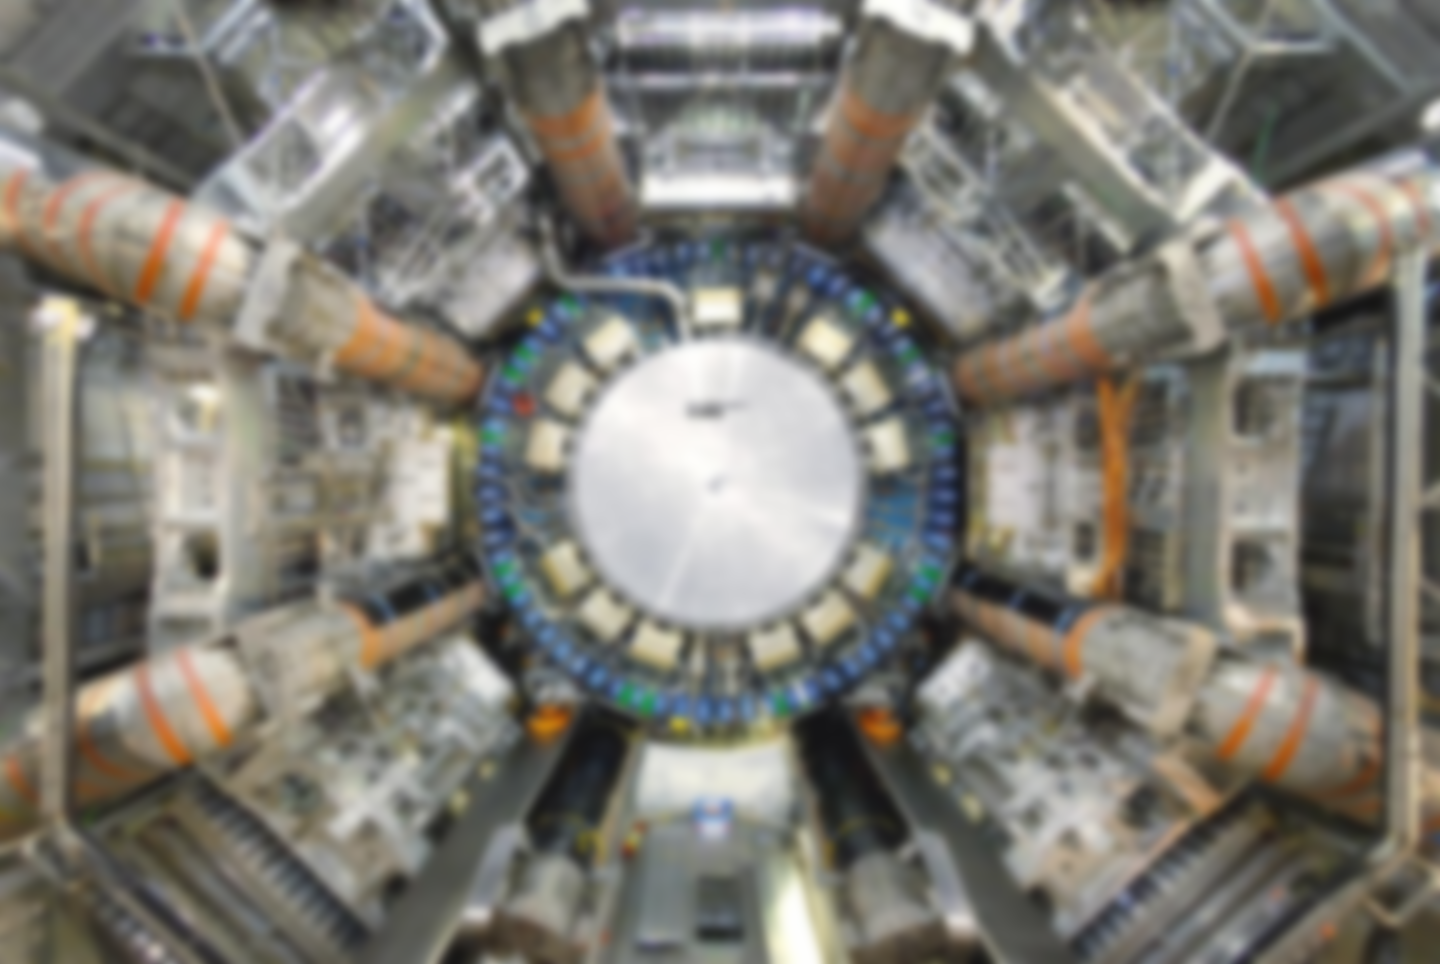
\includegraphics[width=0.8\linewidth]{assets/ATL-TILECAL-SLIDE-2025-552_slide_1_item_1.png}
\end{figure}

\begin{figure}[H]
\centering

\includegraphics[width=0.8\linewidth]{assets/ATL-TILECAL-SLIDE-2025-552_slide_1_item_2.png}
\end{figure}

\begin{figure}[H]
\centering

\includegraphics[width=0.8\linewidth]{assets/ATL-TILECAL-SLIDE-2025-552_slide_1_item_3.jpeg}
\end{figure}

Upgrade of the ATLAS Tile  
Calorimeter Front-End Power

Supply for the HL-LHC

Seyedali Moayedi, on behalf of the ATLAS Tile Calorimeter System

University of Texas at Arlington

Topical Workshop on Electronics for Particle Physics -- 8

October 2025

\section*{Slide 2}

\begin{figure}[H]
\centering

\includegraphics[width=0.8\linewidth]{assets/ATL-TILECAL-SLIDE-2025-552_slide_2_item_1.png}
\end{figure}

Introduction: ATLAS Tile Calorimeter (1)

\begin{figure}[H]
\centering
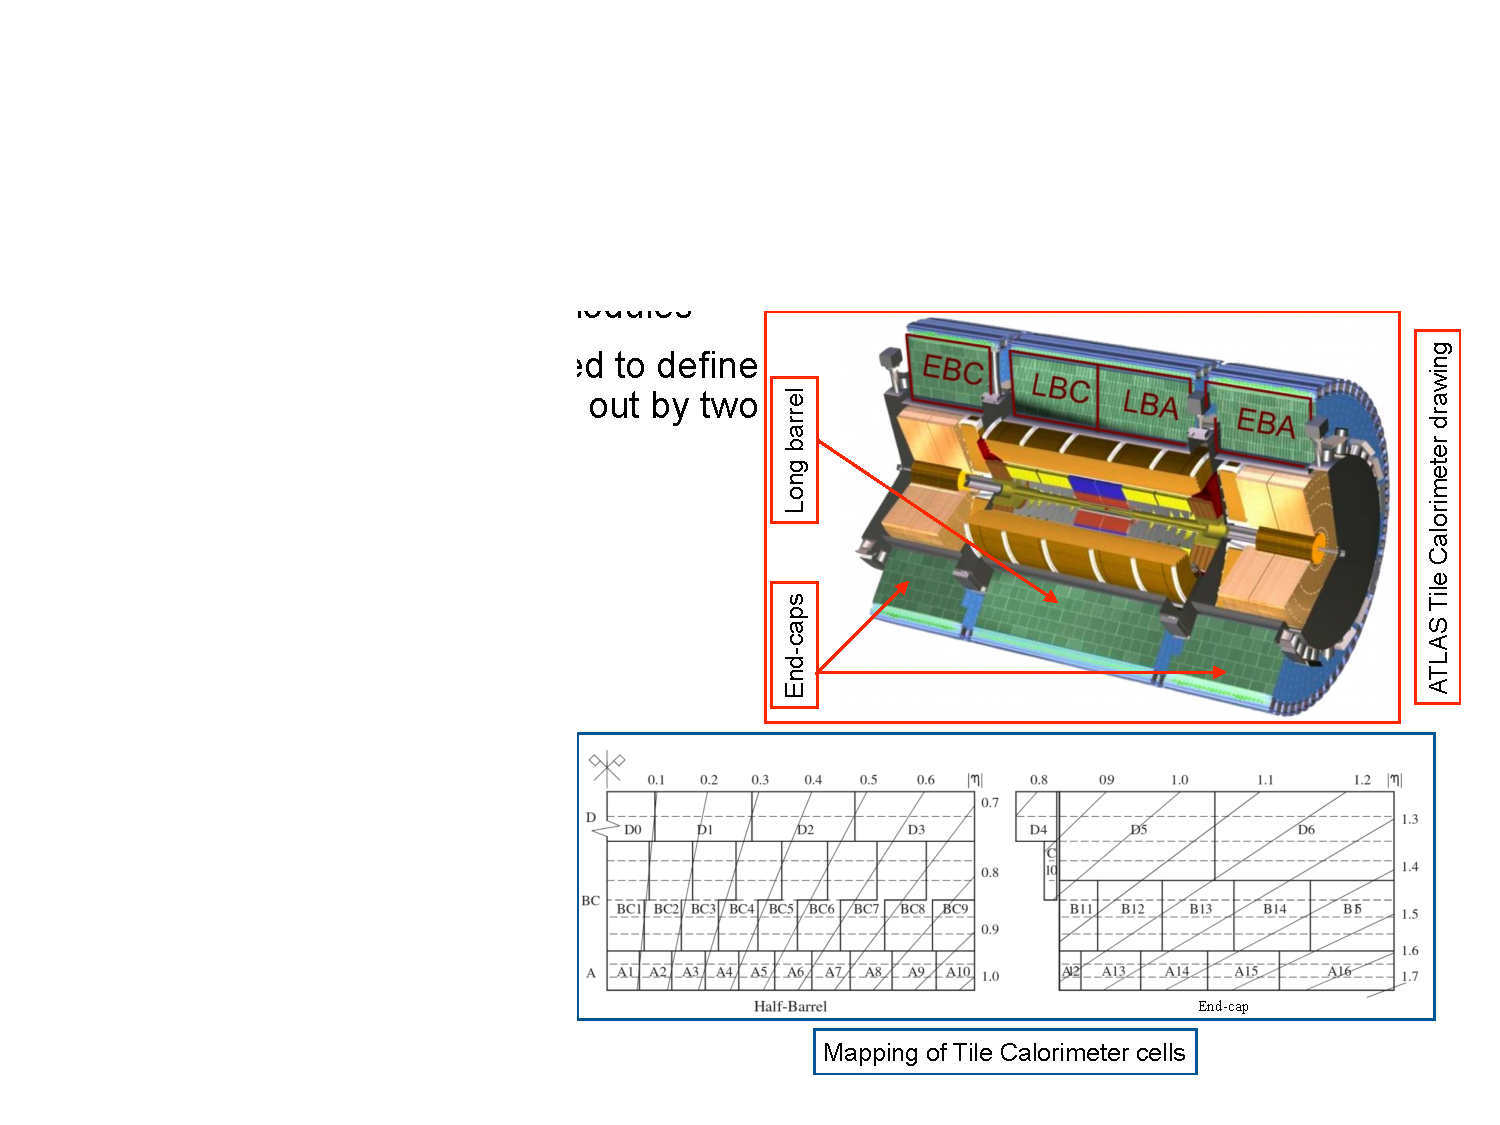
\includegraphics[width=0.8\linewidth]{assets/ATL-TILECAL-SLIDE-2025-552_slide_2_item_2.pdf}
\end{figure}

\begin{figure}[H]
\centering
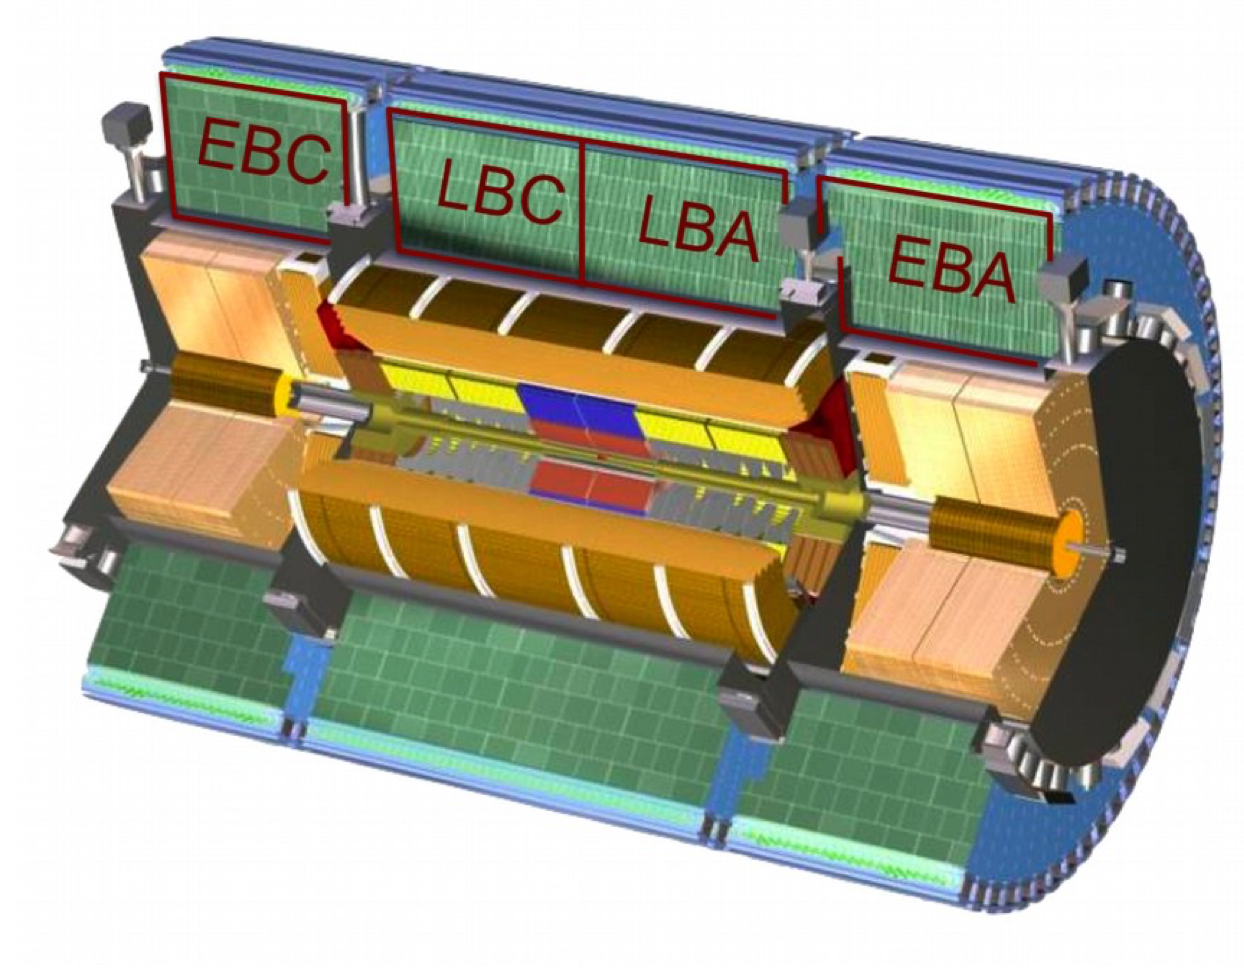
\includegraphics[width=0.8\linewidth]{assets/ATL-TILECAL-SLIDE-2025-552_slide_2_item_3.png}
\end{figure}

\begin{figure}[H]
\centering
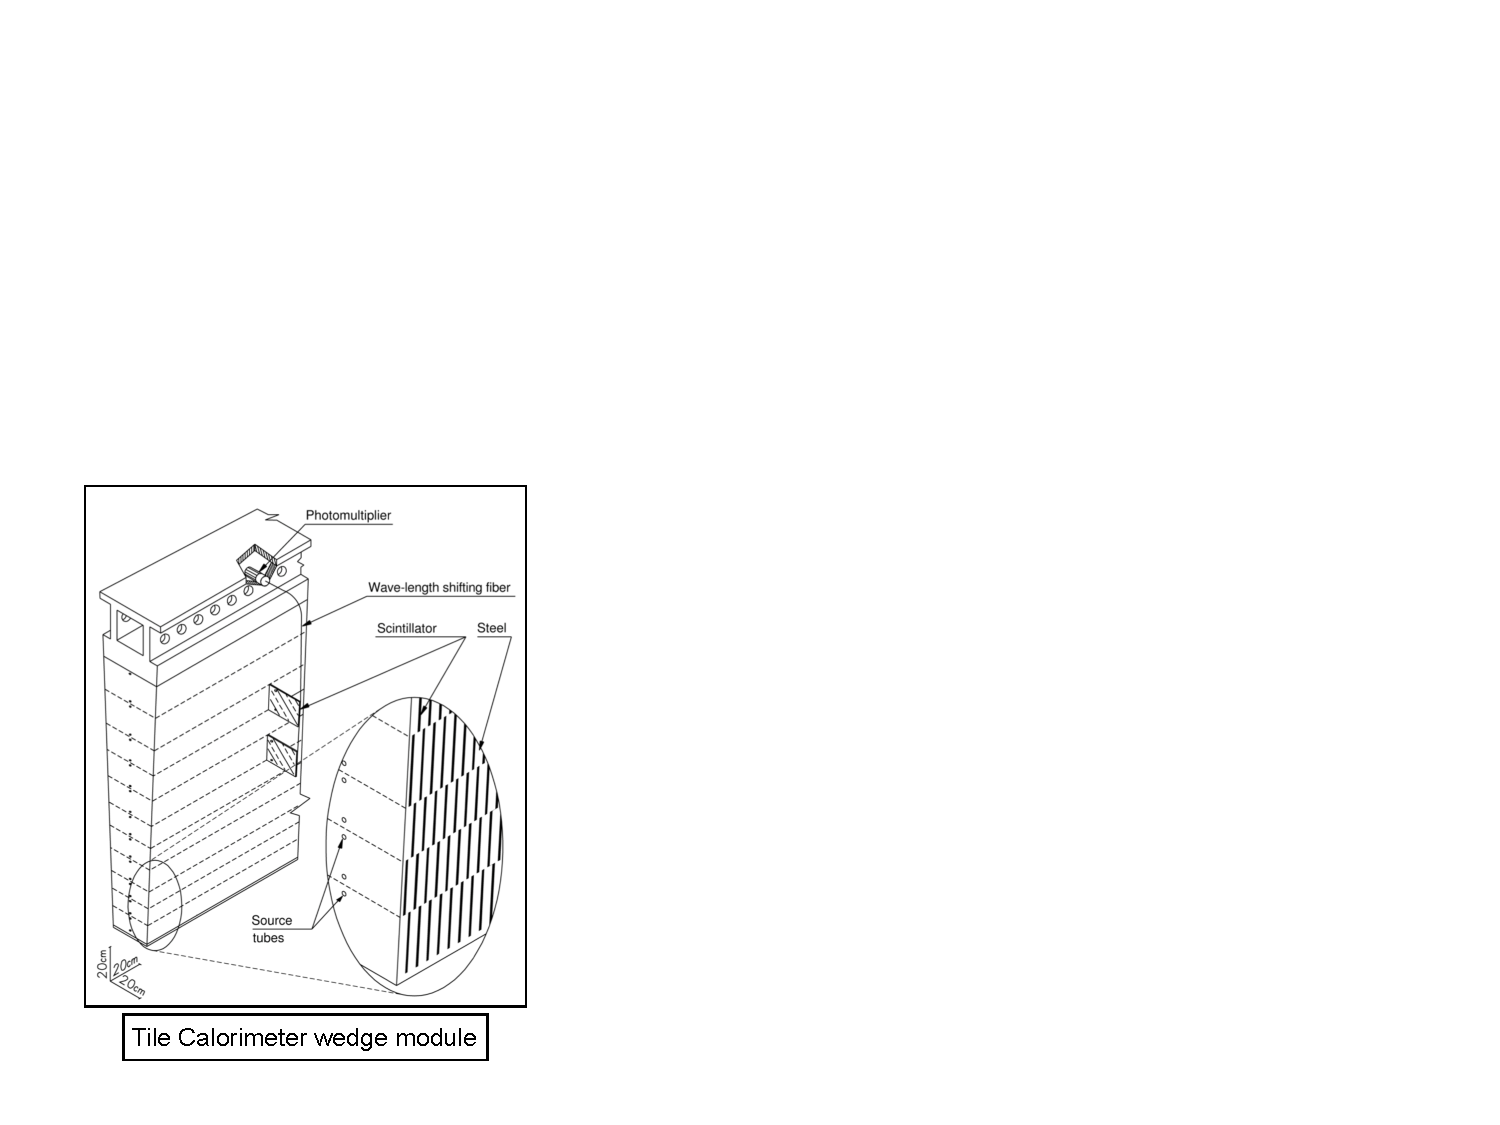
\includegraphics[width=0.8\linewidth]{assets/ATL-TILECAL-SLIDE-2025-552_slide_2_item_4.pdf}
\end{figure}

\begin{figure}[H]
\centering
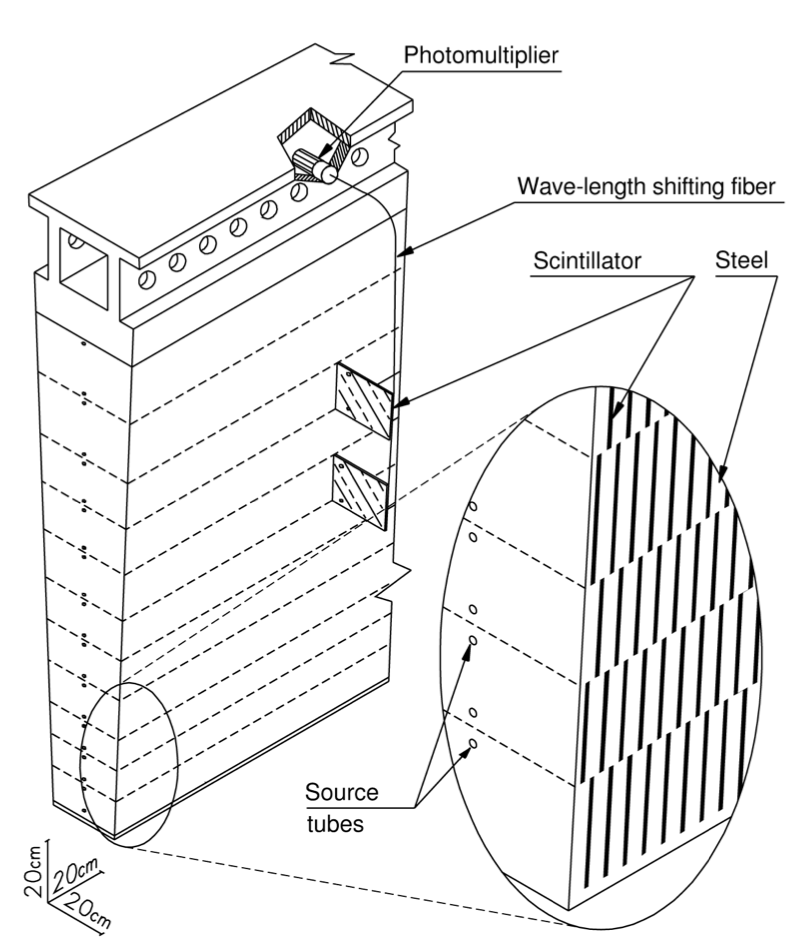
\includegraphics[width=0.8\linewidth]{assets/ATL-TILECAL-SLIDE-2025-552_slide_2_item_5.png}
\end{figure}

\begin{figure}[H]
\centering
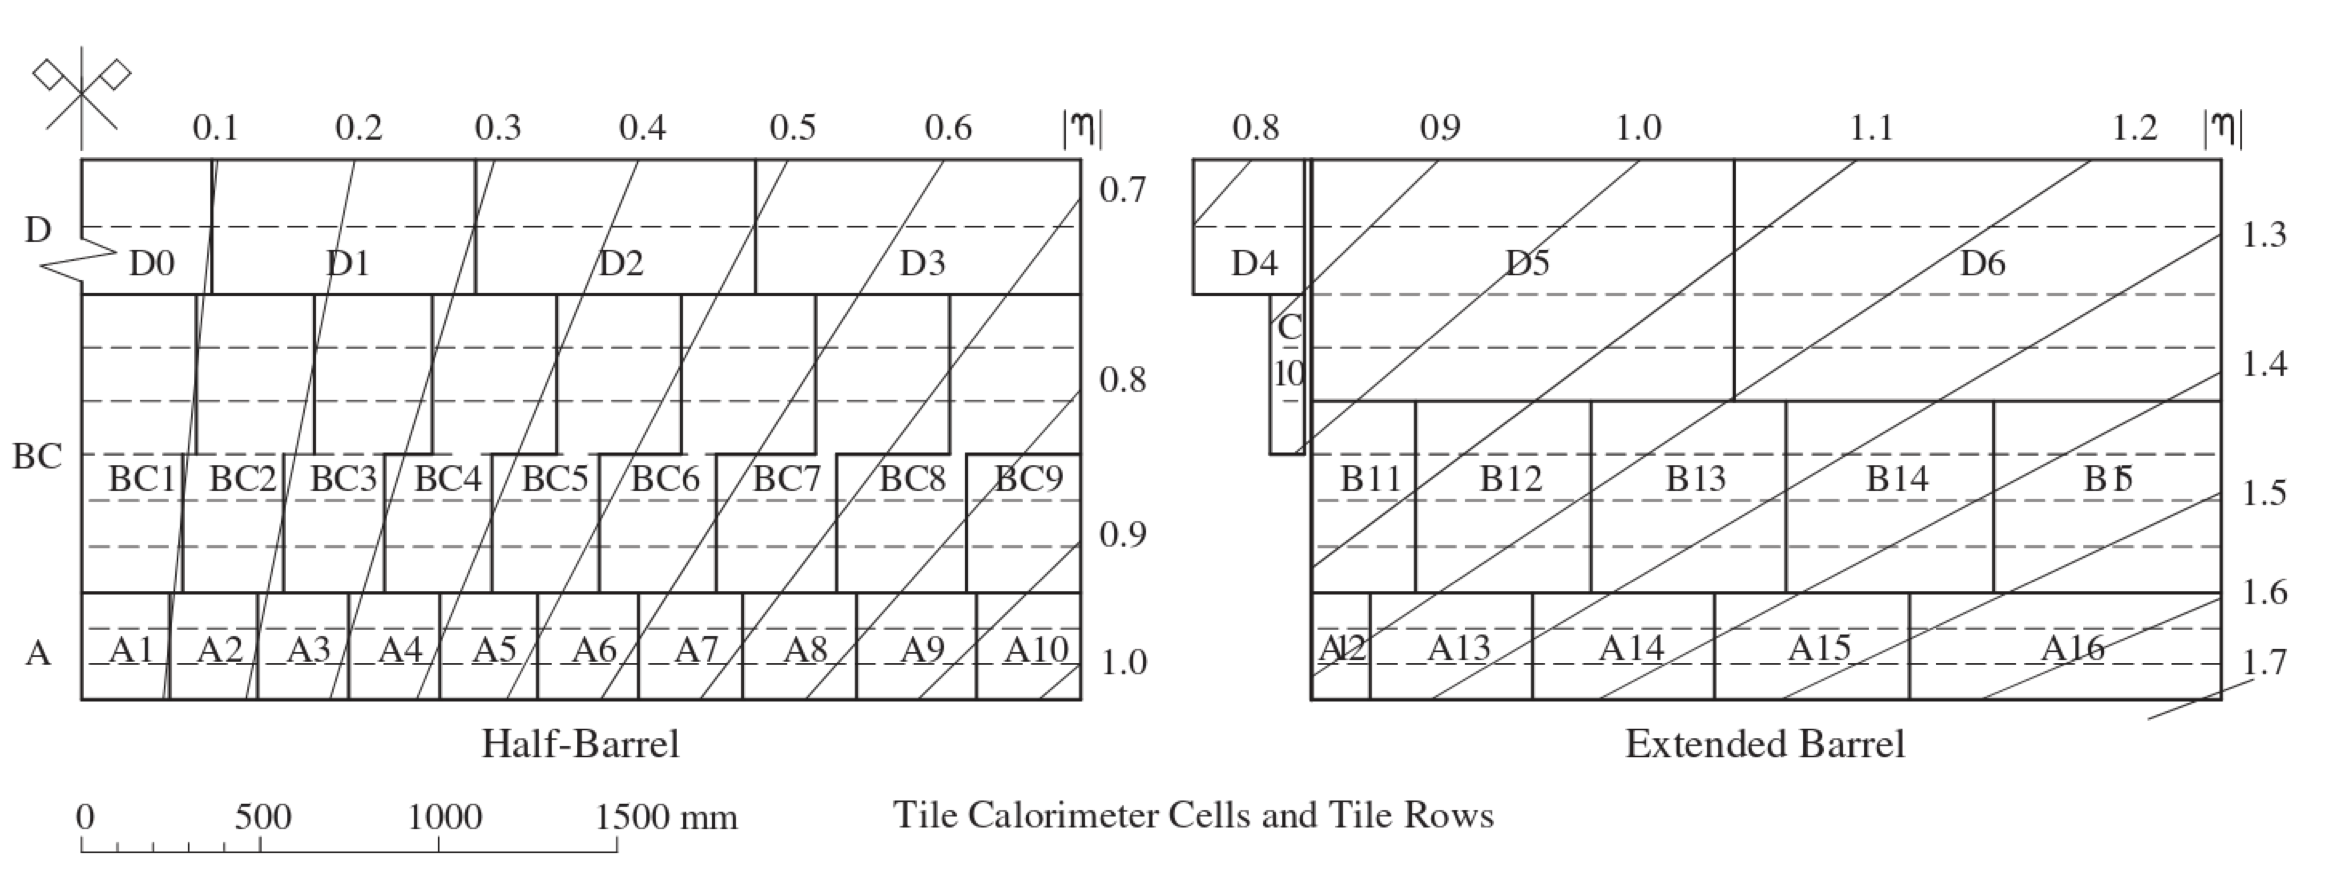
\includegraphics[width=0.8\linewidth]{assets/ATL-TILECAL-SLIDE-2025-552_slide_2_item_6.png}
\end{figure}

Seyedali Moayedi

Topical Workshop on Electronics for Particle Physics -- 8 October 2025

2

\section*{Slide 3}

\begin{figure}[H]
\centering

\includegraphics[width=0.8\linewidth]{assets/ATL-TILECAL-SLIDE-2025-552_slide_3_item_1.png}
\end{figure}

Introduction: ATLAS Tile Calorimeter (2)

   In total, there are 256 modules in Tile Calorimeter

   The Low Voltage Power Supplies (LVPS) are located inside a box in the  
``finger'' of each module and provide power to front-end electronics to  
read out PMT signals

\begin{figure}[H]
\centering
\includegraphics[width=0.8\linewidth]{assets/ATL-TILECAL-SLIDE-2025-552_slide_3_item_2.pdf}
\end{figure}

\begin{figure}[H]
\centering
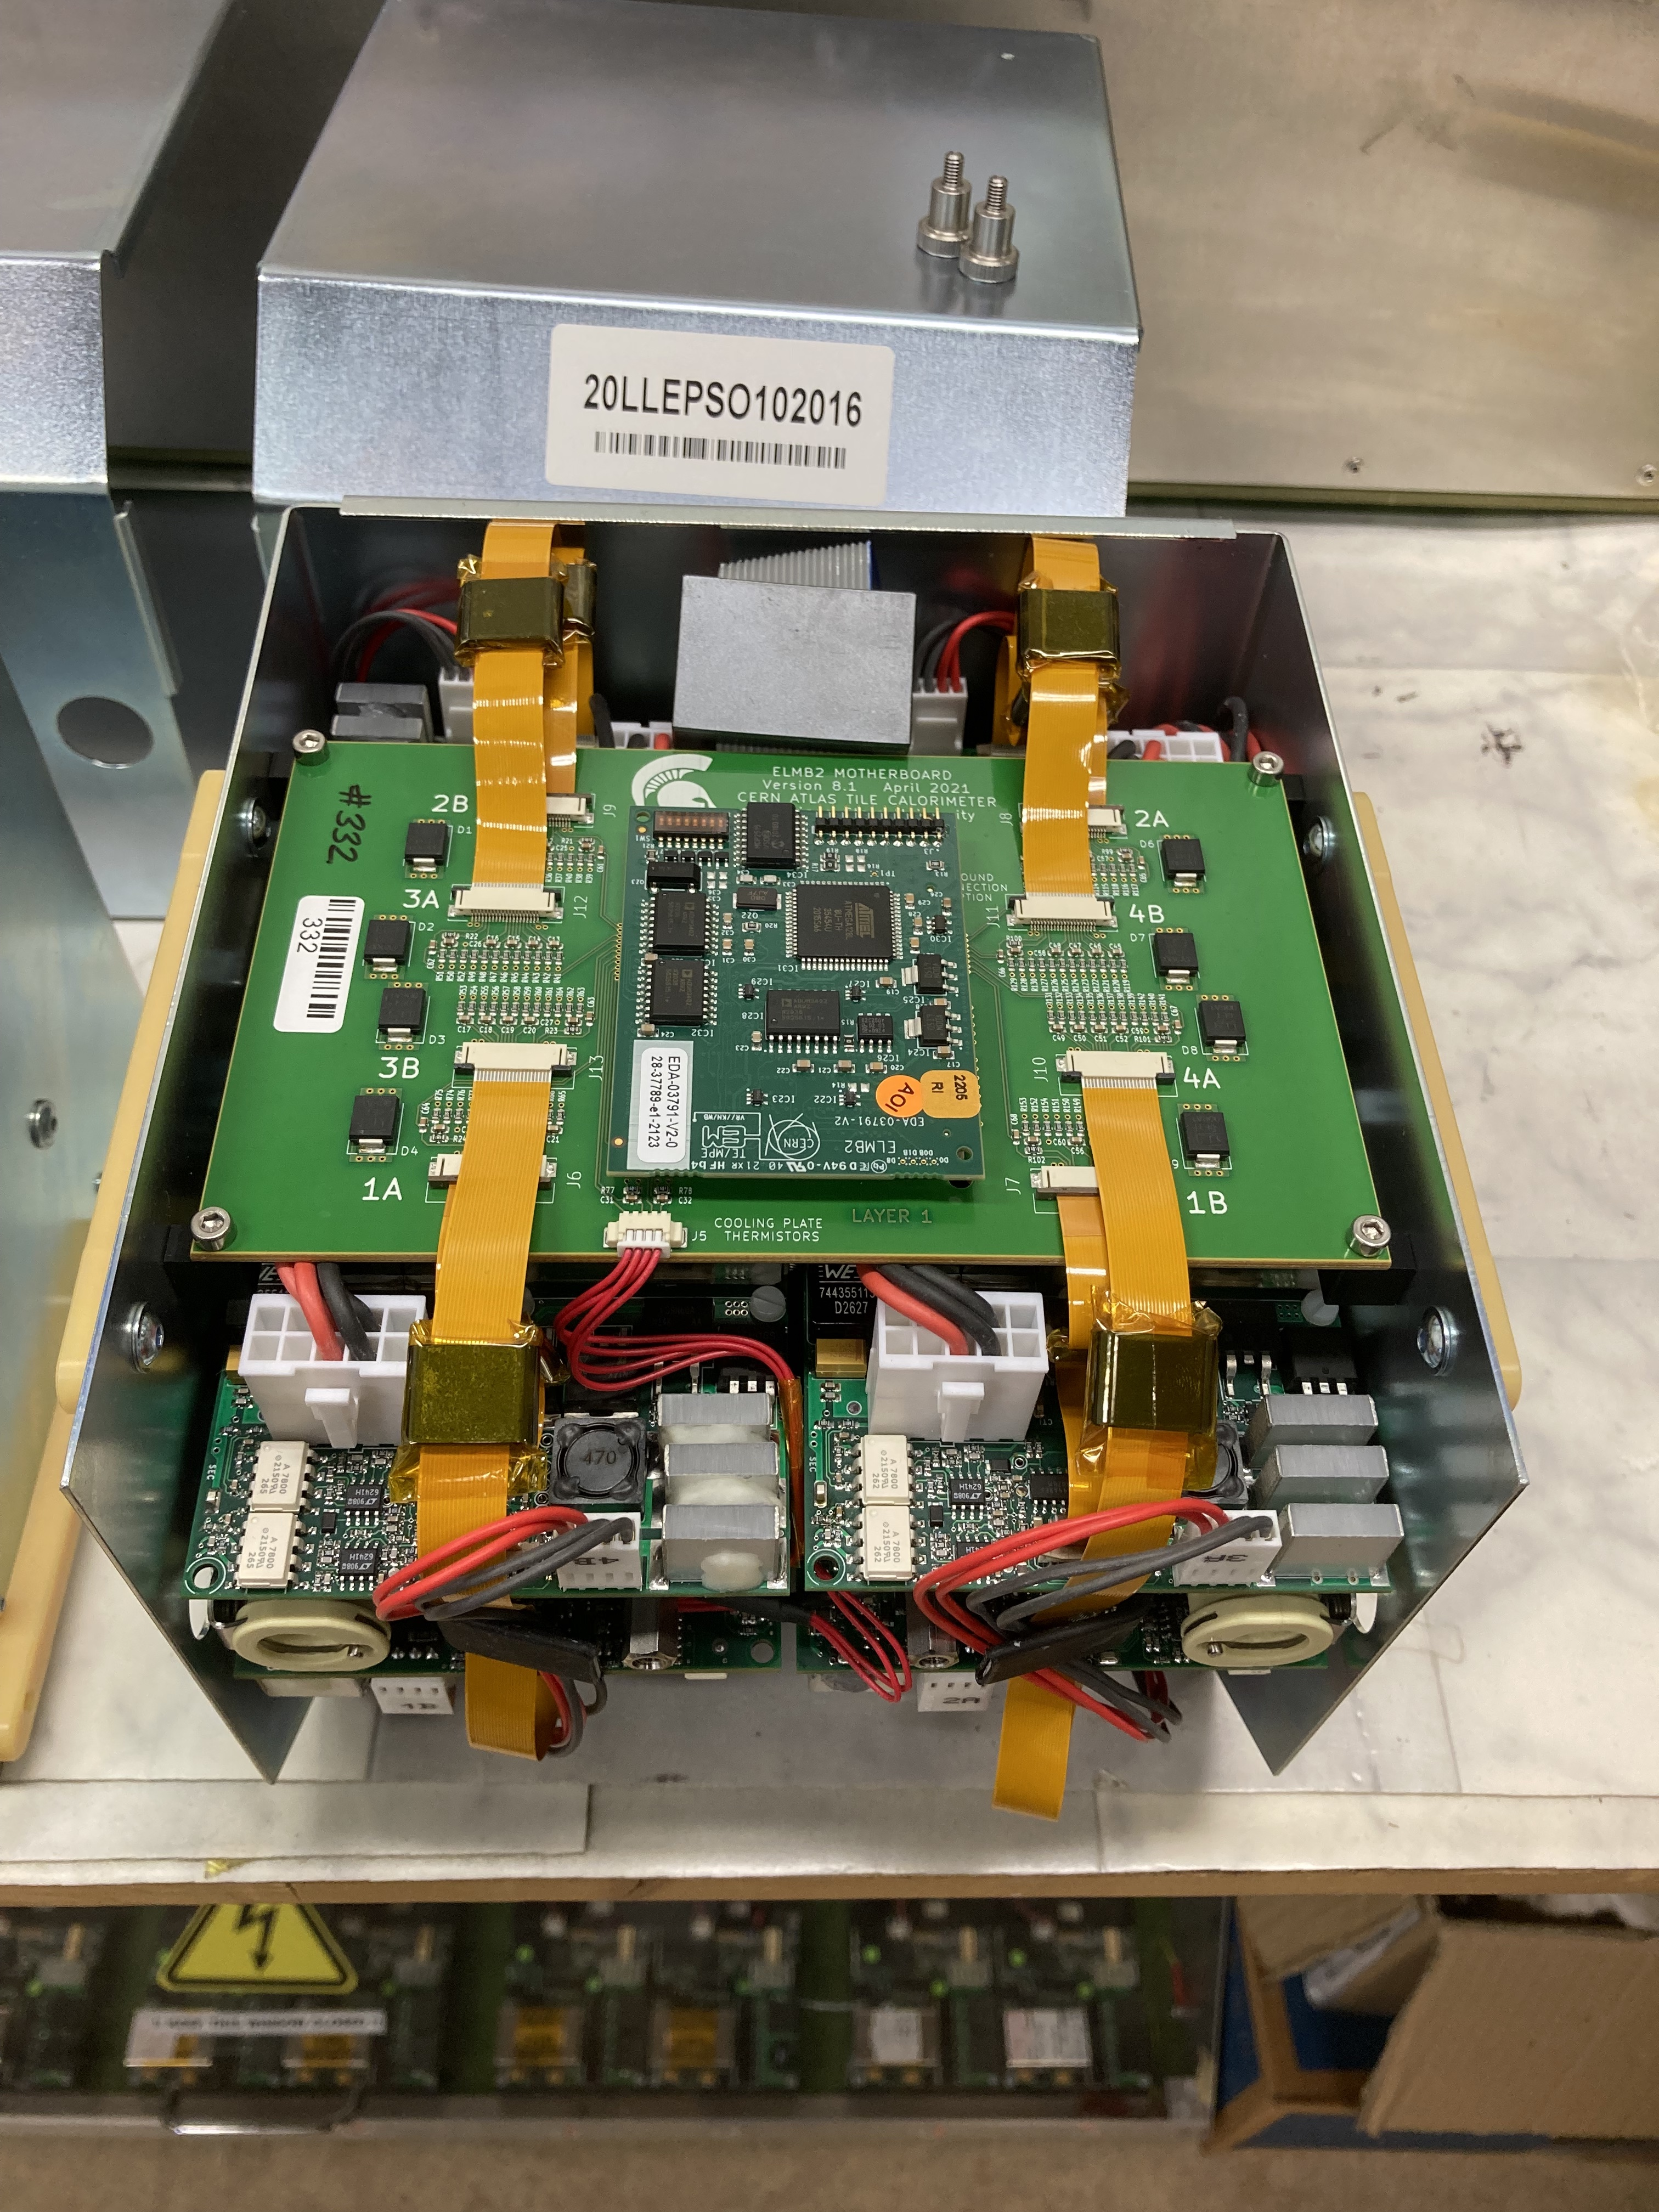
\includegraphics[width=0.8\linewidth]{assets/ATL-TILECAL-SLIDE-2025-552_slide_3_item_3.jpeg}
\end{figure}

\begin{figure}[H]
\centering
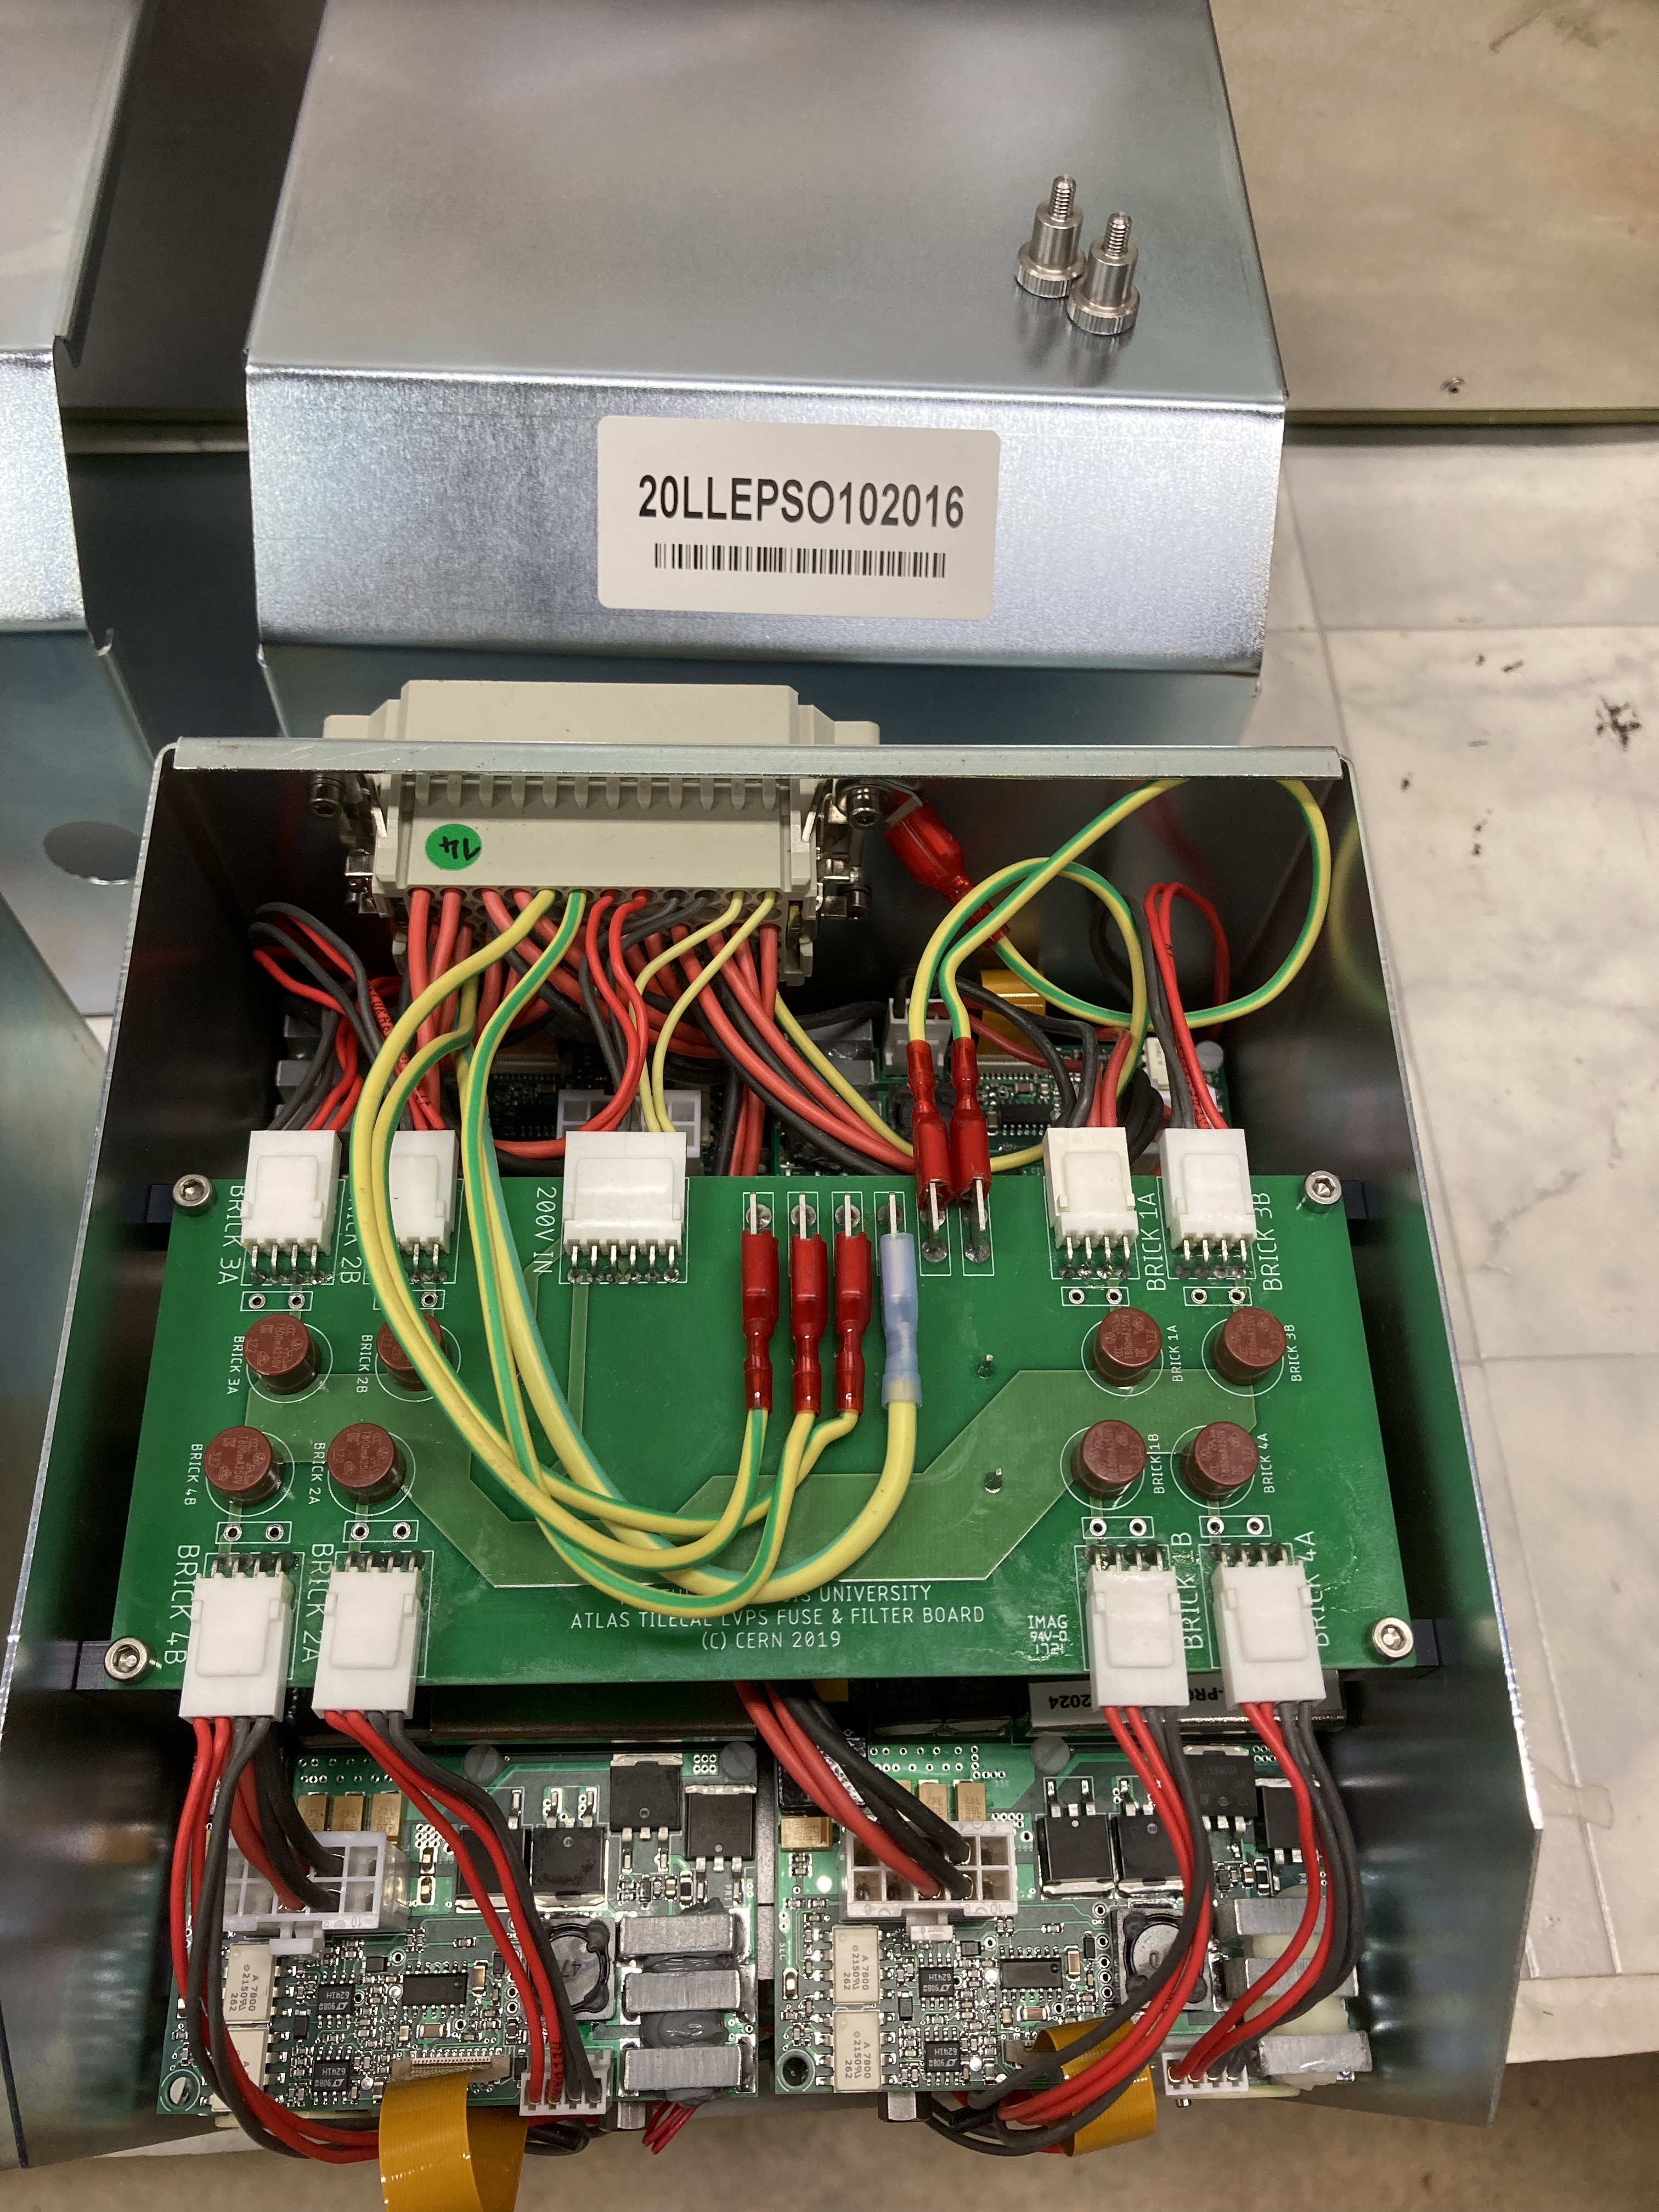
\includegraphics[width=0.8\linewidth]{assets/ATL-TILECAL-SLIDE-2025-552_slide_3_item_4.jpeg}
\end{figure}

\begin{figure}[H]
\centering
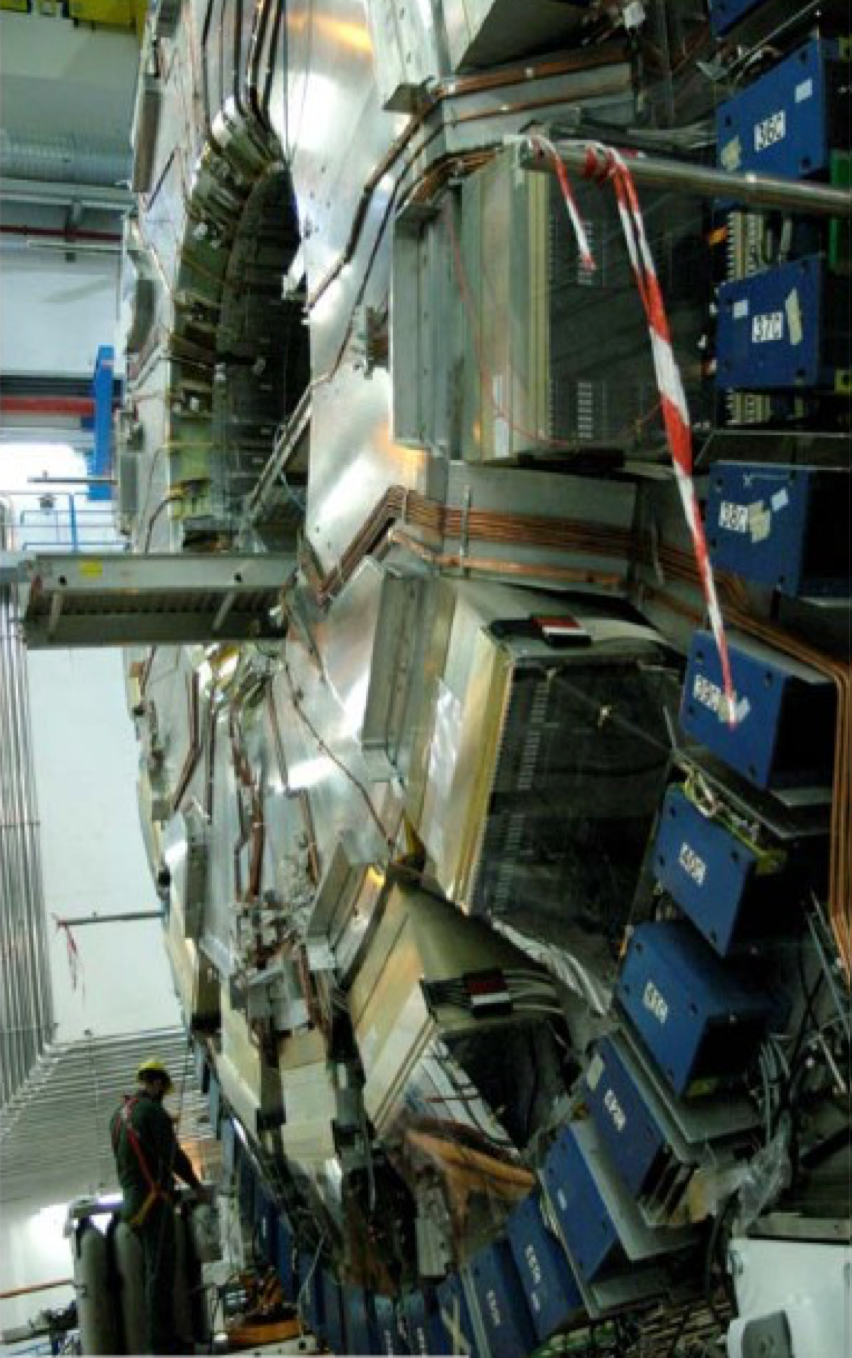
\includegraphics[width=0.8\linewidth]{assets/ATL-TILECAL-SLIDE-2025-552_slide_3_item_5.png}
\end{figure}

\begin{figure}[H]
\centering
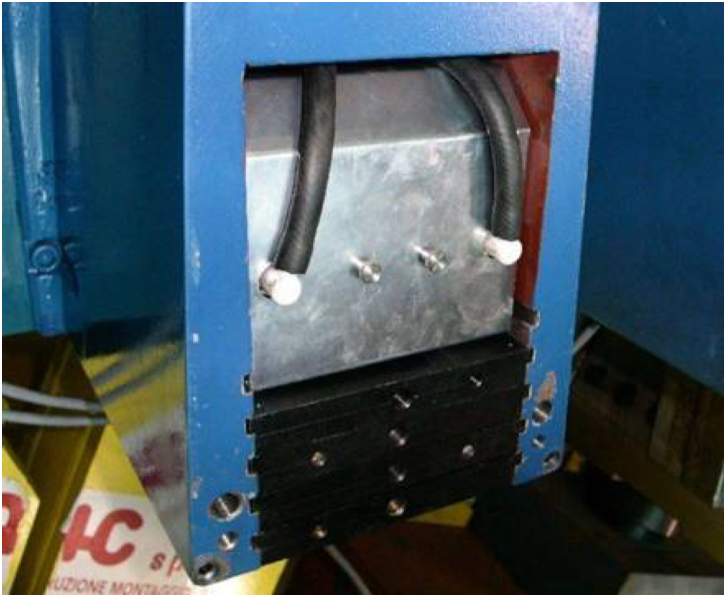
\includegraphics[width=0.8\linewidth]{assets/ATL-TILECAL-SLIDE-2025-552_slide_3_item_6.png}
\end{figure}

Seyedali Moayedi

Topical Workshop on Electronics for Particle Physics -- 8 October 2025

3

\section*{Slide 4}

\begin{figure}[H]
\centering

\includegraphics[width=0.8\linewidth]{assets/ATL-TILECAL-SLIDE-2025-552_slide_4_item_1.png}
\end{figure}

Tile Calorimeter Power Supplies: LVPS Bricks

   The LVPS bricks are switching DC-DC converters with a topology of      
two-switch forward converter and a switching frequency of 300 kHz

   In the legacy system, 8 different bricks inside the box provide power to  
each module of the Tile Calorimeter at 8 different voltage levels, but in the  
phase-2 upgrade system (for HL-LHC), all 8 bricks in a module will convert  
the 200 V input to a nominal 10 V output at a nominal power of 23 W

   Point of load regulators on front-end electronics provide different voltages

\begin{figure}[H]
\centering
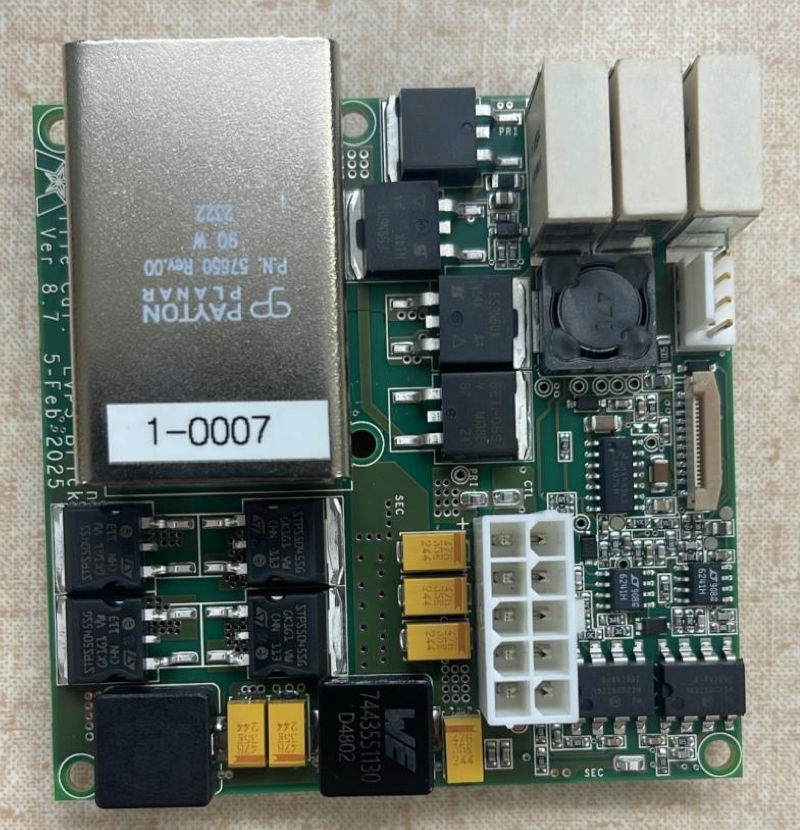
\includegraphics[width=0.8\linewidth]{assets/ATL-TILECAL-SLIDE-2025-552_slide_4_item_2.png}
\end{figure}

\begin{figure}[H]
\centering
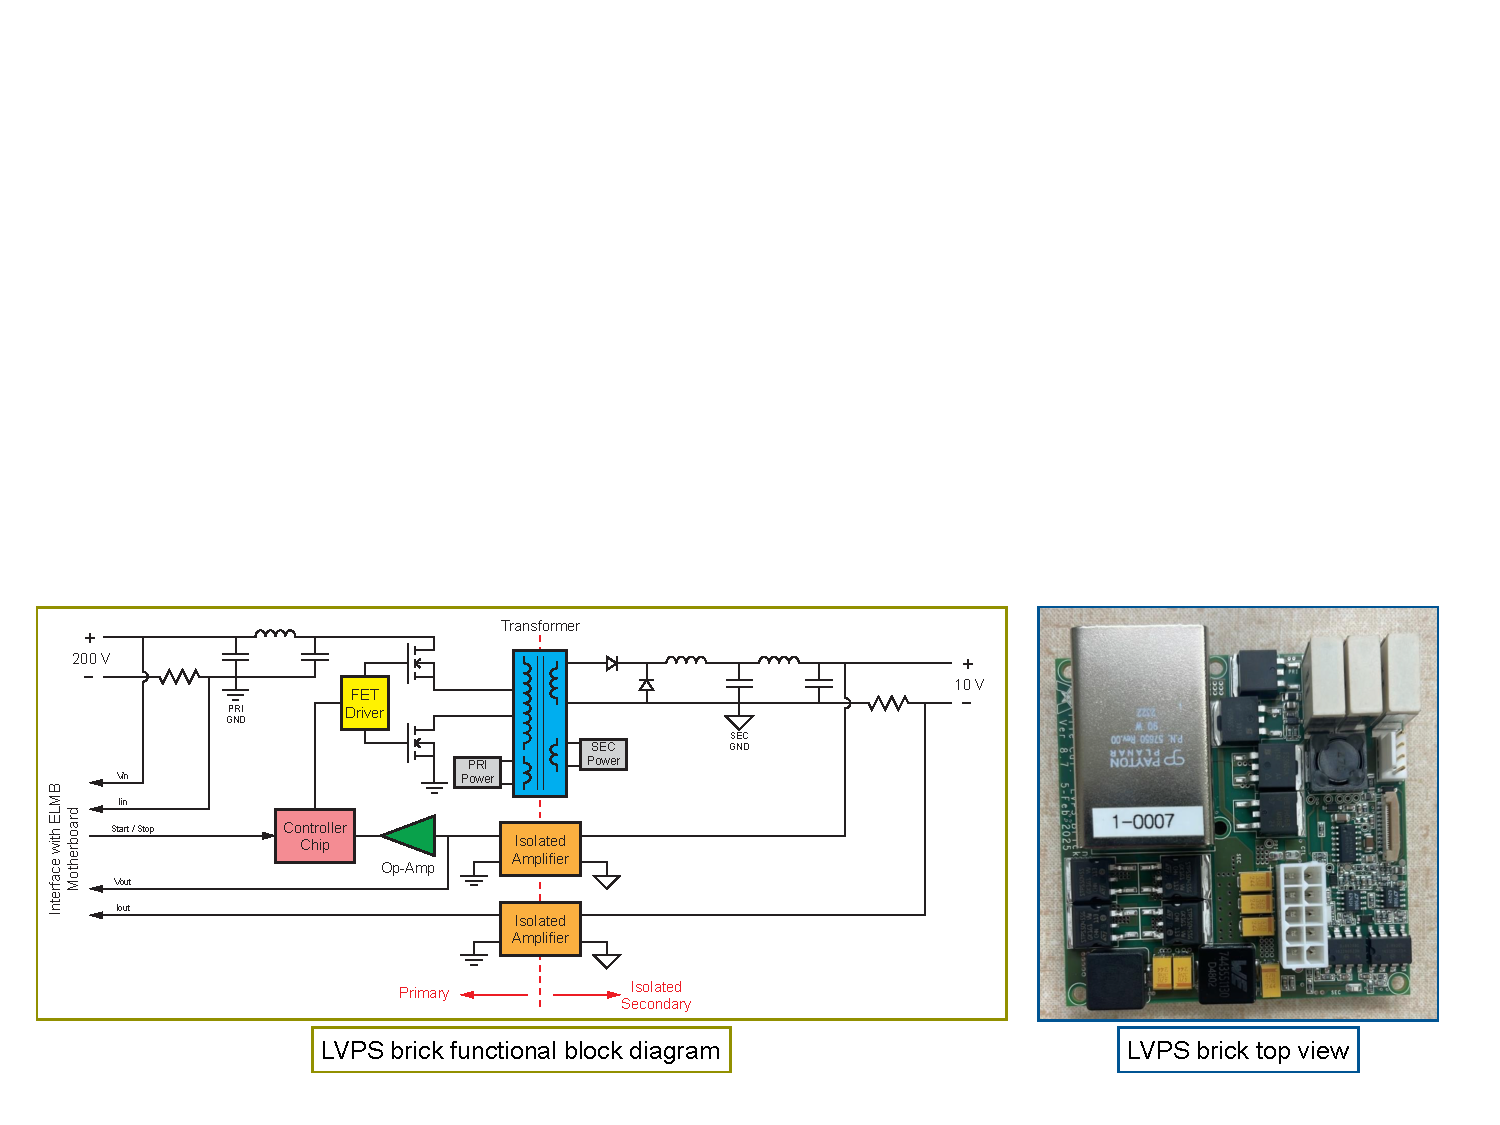
\includegraphics[width=0.8\linewidth]{assets/ATL-TILECAL-SLIDE-2025-552_slide_4_item_3.pdf}
\end{figure}

Seyedali Moayedi

Topical Workshop on Electronics for Particle Physics -- 8 October 2025

4

\section*{Slide 5}

\begin{figure}[H]
\centering

\includegraphics[width=0.8\linewidth]{assets/ATL-TILECAL-SLIDE-2025-552_slide_5_item_1.png}
\end{figure}

Radiation Criteria

   In Tile Calorimeter, the fingers, where LVPS bricks are located at, are       
the harshest location in terms of radiation

   The very early design of the bricks were showing excessive trips, so a  
customized rad-hard design for these bricks is essential

   Based on the new guidelines and simulations performed in 2020, the  
radiation criteria were updated

\begin{figure}[H]
\centering
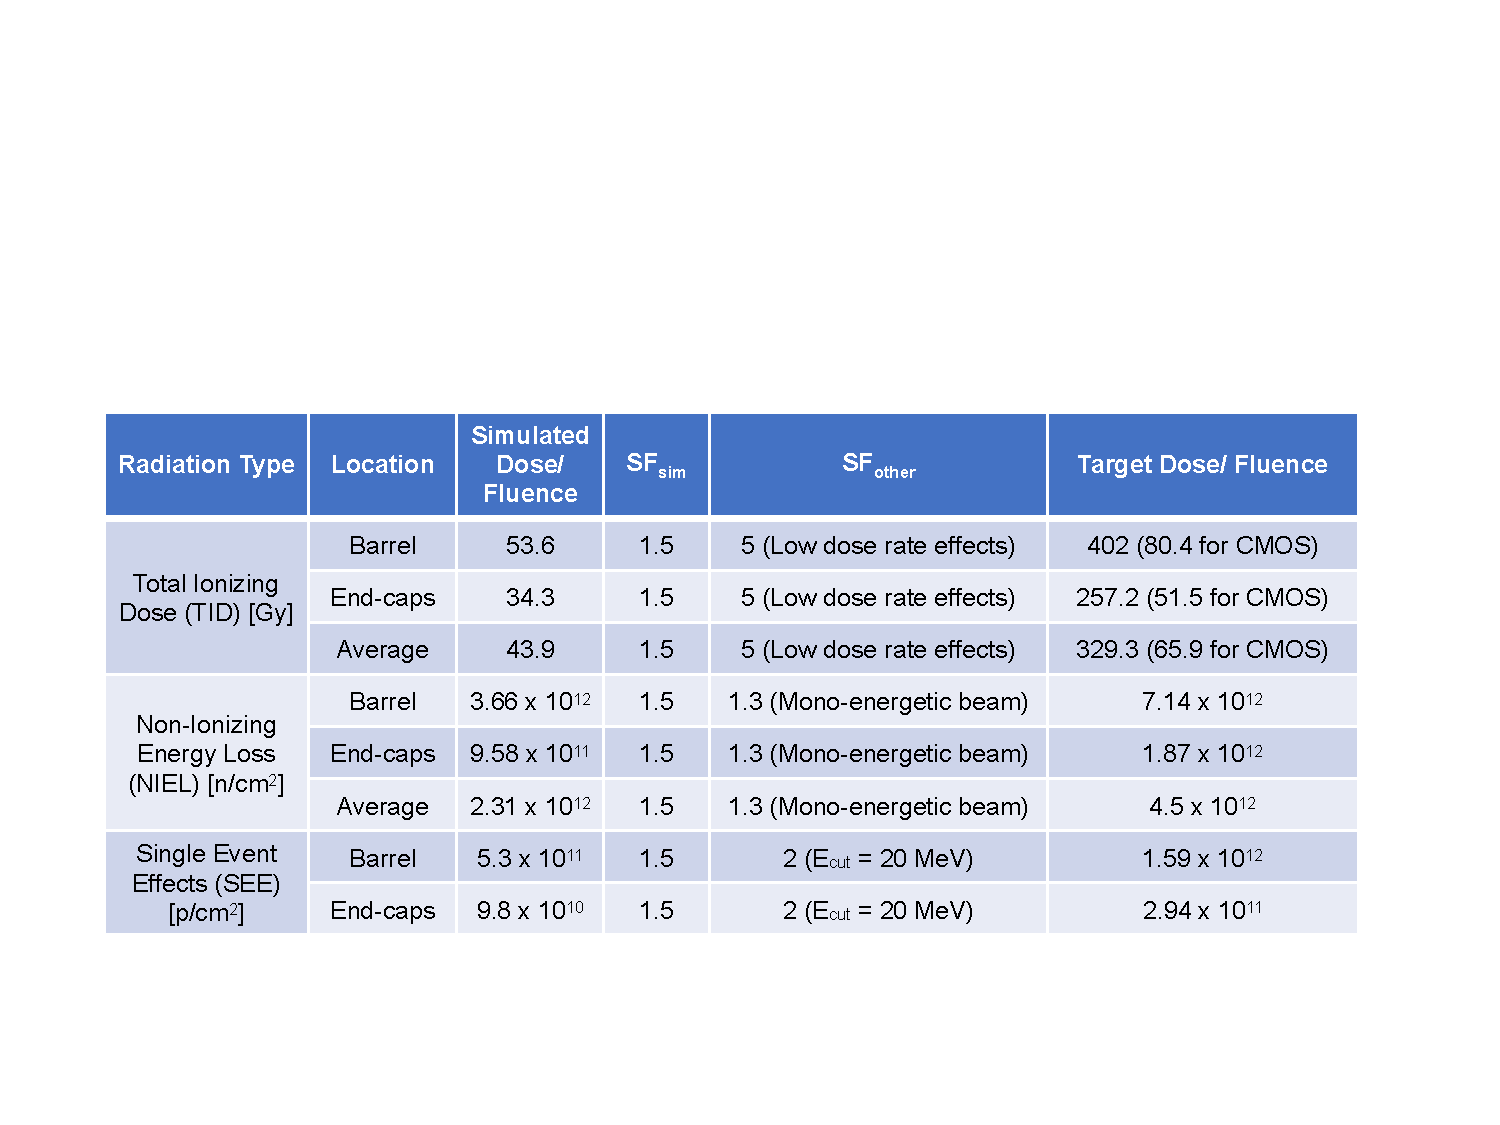
\includegraphics[width=0.8\linewidth]{assets/ATL-TILECAL-SLIDE-2025-552_slide_5_item_2.pdf}
\end{figure}

Seyedali Moayedi

Topical Workshop on Electronics for Particle Physics -- 8 October 2025

5

\section*{Slide 6}

\begin{figure}[H]
\centering

\includegraphics[width=0.8\linewidth]{assets/ATL-TILECAL-SLIDE-2025-552_slide_6_item_1.png}
\end{figure}

Main Design Improvements

   As there were some issues with efficiency and thermal management     
of the bricks, two components were studied to be replaced

   The original power MOSFETs (STB57N65M5) caused high switching  
losses and was replaced by SIHFS9N60A

   The new MOSFET caused a significant increase in the efficiency of  
the bricks (from \textasciitilde{}58\% to \textasciitilde{}72\%)

   The new MOSFET had a 65\% smaller gate-source capacitance 
 
   The output inductor was getting a bit hot, and was replaced with an  
inductor with smaller series resistance
 
   The improvement in the efficiency helped with the limitations of the  
cooling system

   A brick efficiency of at least 65\% was required for the cooling plant with  
77 kW capacity

   Due to limitation in cabling from the service room to the modules, the  
number of signals for controlling each brick had to be reduced

\begin{figure}[H]
\centering
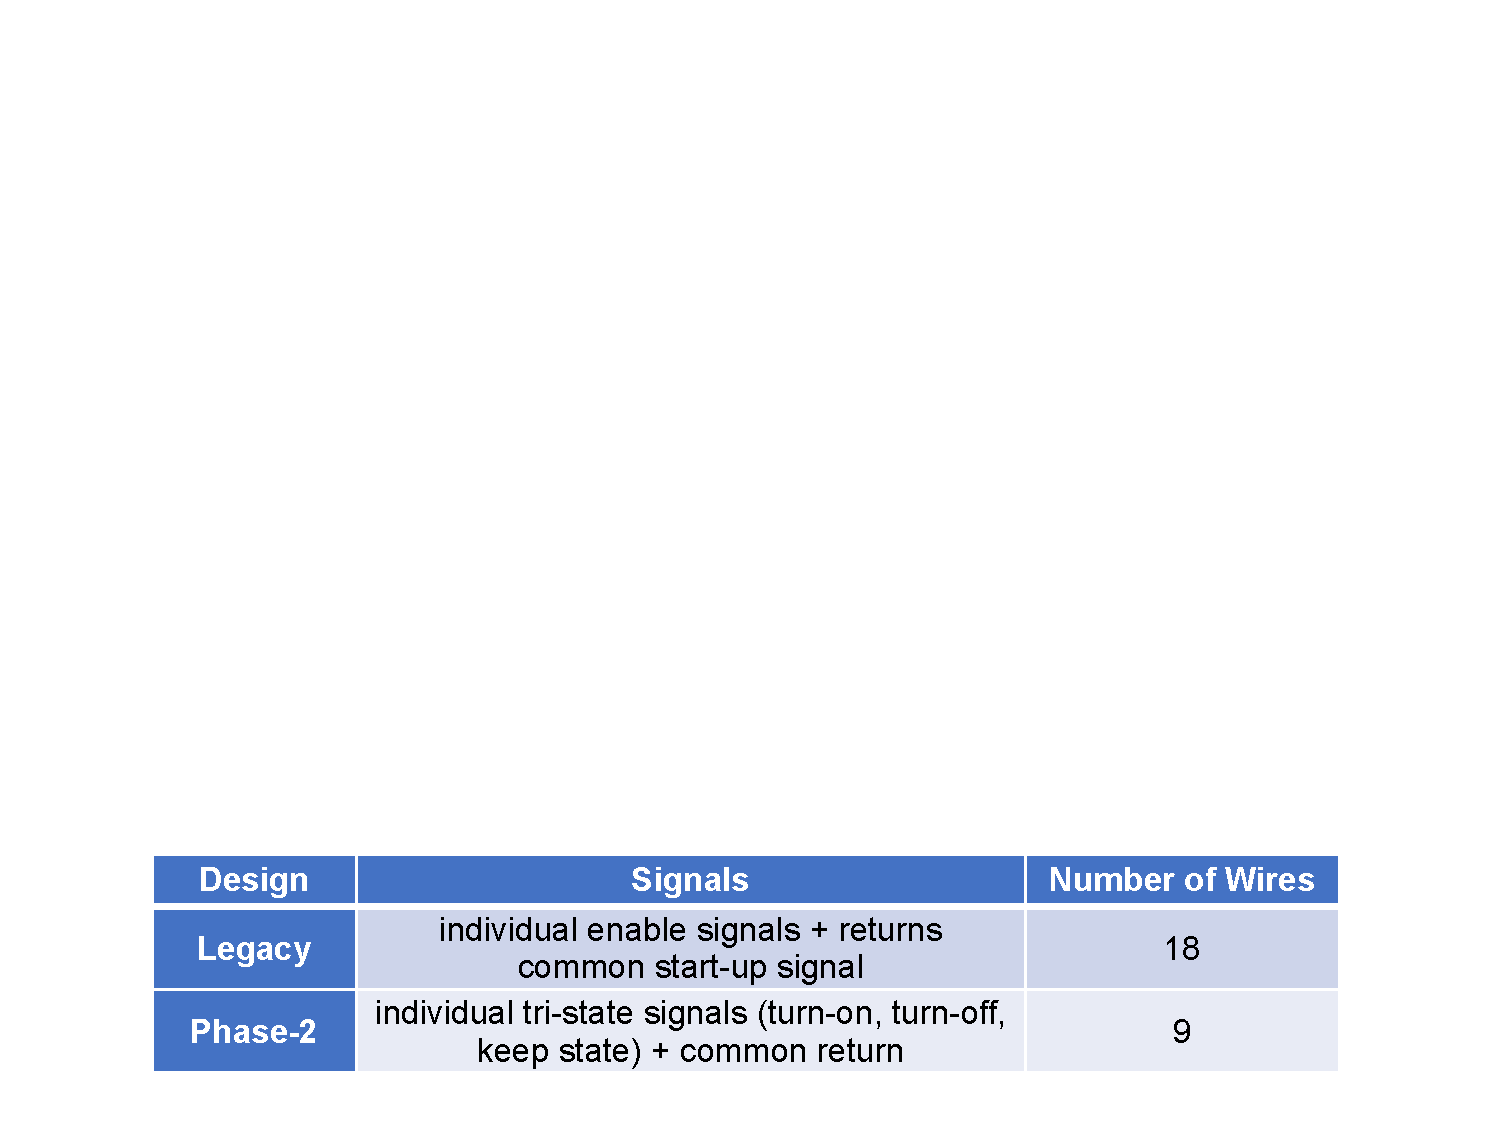
\includegraphics[width=0.8\linewidth]{assets/ATL-TILECAL-SLIDE-2025-552_slide_6_item_2.pdf}
\end{figure}

Seyedali Moayedi

Topical Workshop on Electronics for Particle Physics -- 8 October 2025

6

\section*{Slide 7}

\begin{figure}[H]
\centering

\includegraphics[width=0.8\linewidth]{assets/ATL-TILECAL-SLIDE-2025-552_slide_7_item_1.png}
\end{figure}

Radiation Tests Overview

   Some tests had been performed on the components by 2020, but as   
the new guidelines were suggesting, batch-to-batch safety factor was  
not applicable anymore, and each batch used on the final boards,  
should have been tested

   Procurement of components from single (or limited) batch(es) was  
started in 2021, following the initial radiation tests in 2018-2020

\begin{figure}[H]
\centering
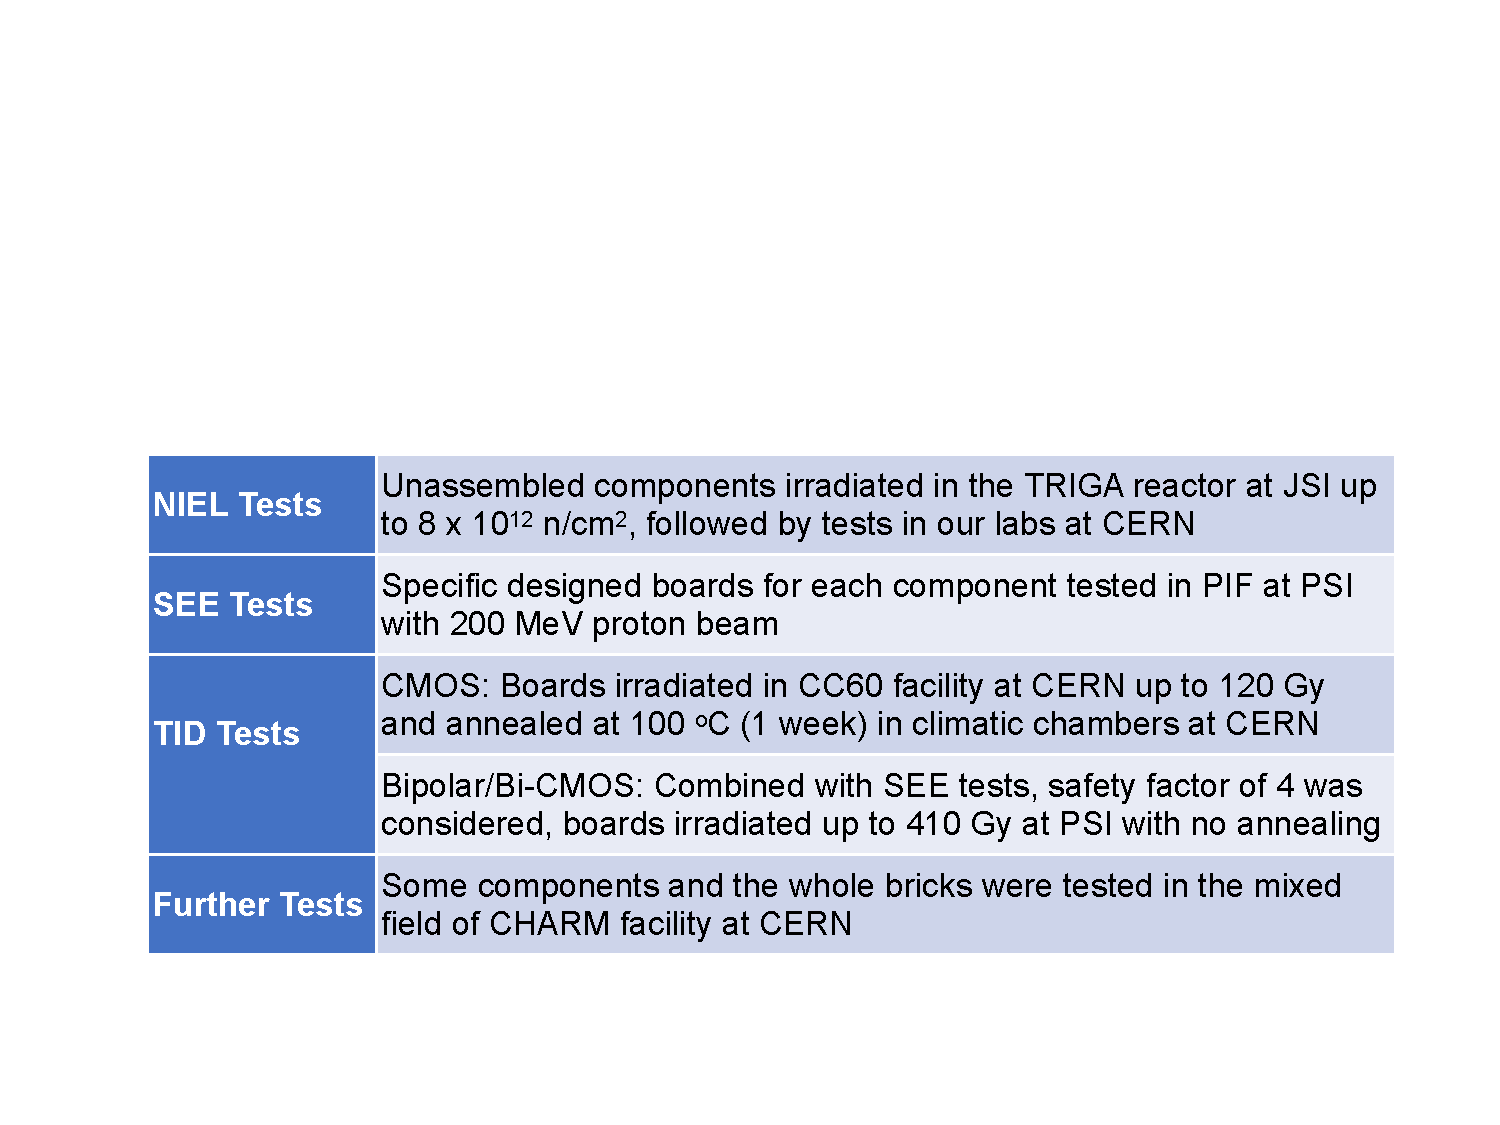
\includegraphics[width=0.8\linewidth]{assets/ATL-TILECAL-SLIDE-2025-552_slide_7_item_2.pdf}
\end{figure}

JSI : Jozef Stefan Institute (Ljubljana)    TRIGA : Training, Research, Isotopes, General Atomics
 
PIF : Proton Irradiation Facility    PSI : Paul Scherrer Institute (Villigen)    CC60 : CERN Cobalt-60

CHARM : CERN Highly-Accelerated Mixed Field

Seyedali Moayedi

Topical Workshop on Electronics for Particle Physics -- 8 October 2025

7

\section*{Slide 8}

\begin{figure}[H]
\centering

\includegraphics[width=0.8\linewidth]{assets/ATL-TILECAL-SLIDE-2025-552_slide_8_item_1.png}
\end{figure}

Radiation Tests: Diodes (1)

   Seven different diodes were tested

   MURS160T3G, STPS1L30MF, STPS1L60MF, STPS5045, BAT46,  
VS-8ETH06, and SMCJ15A (TVS Diode)

   For the TVS diode (SMCJ15A), the TID tests were performed by biasing  
them at stand-off voltage during the beam time

   During the stop time, a relay board was used to go through the  
diode array and conduct a reverse current and measure the  
breakdown voltage for each diode

   Performed at a flux of 2.85 Gy/h,  TID tests were successful

\begin{figure}[H]
\centering
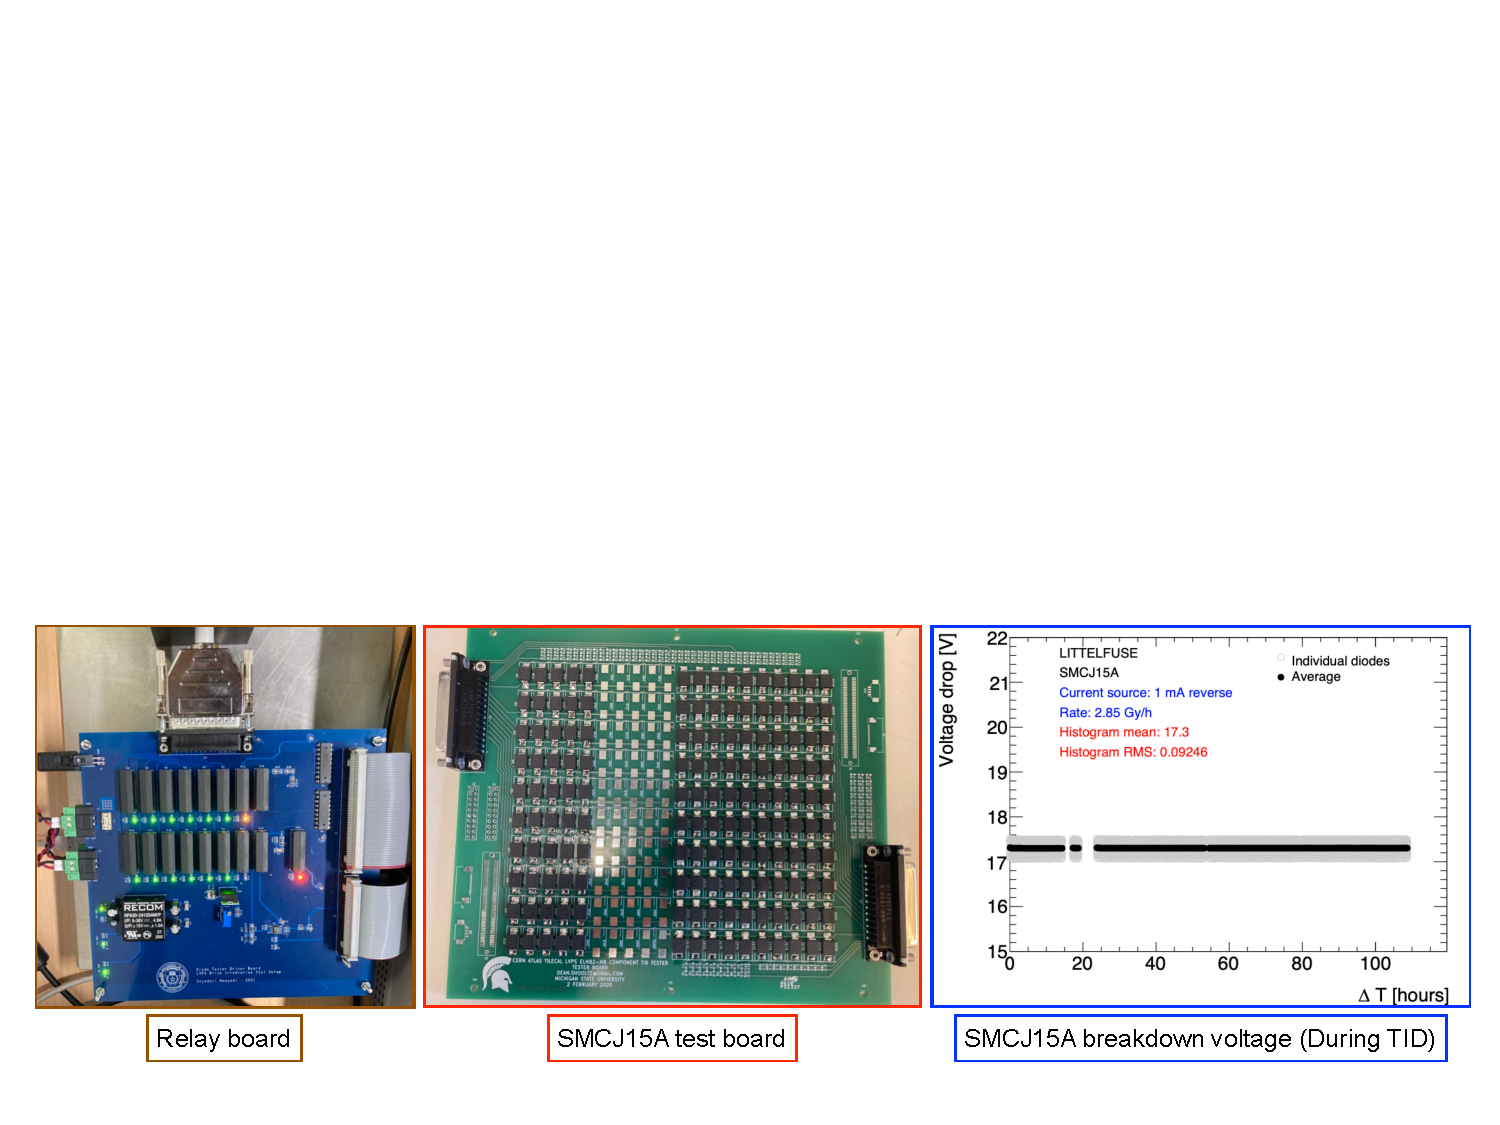
\includegraphics[width=0.8\linewidth]{assets/ATL-TILECAL-SLIDE-2025-552_slide_8_item_2.pdf}
\end{figure}

\begin{figure}[H]
\centering
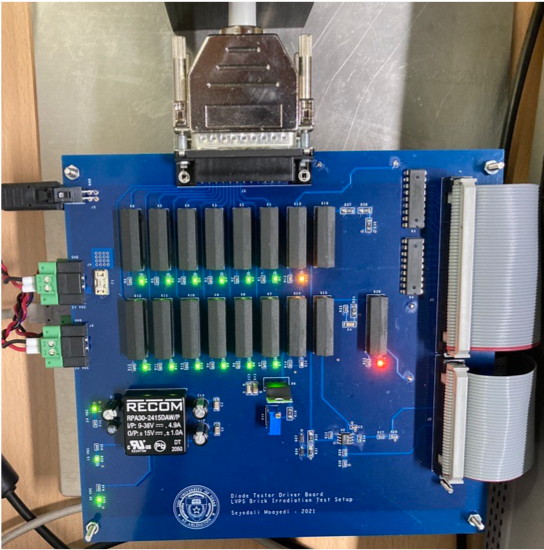
\includegraphics[width=0.8\linewidth]{assets/ATL-TILECAL-SLIDE-2025-552_slide_8_item_3.png}
\end{figure}

\begin{figure}[H]
\centering
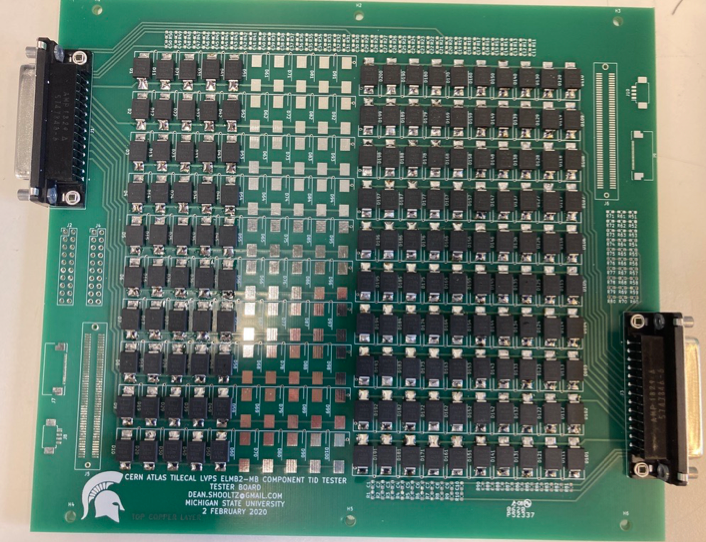
\includegraphics[width=0.8\linewidth]{assets/ATL-TILECAL-SLIDE-2025-552_slide_8_item_4.png}
\end{figure}

\begin{figure}[H]
\centering
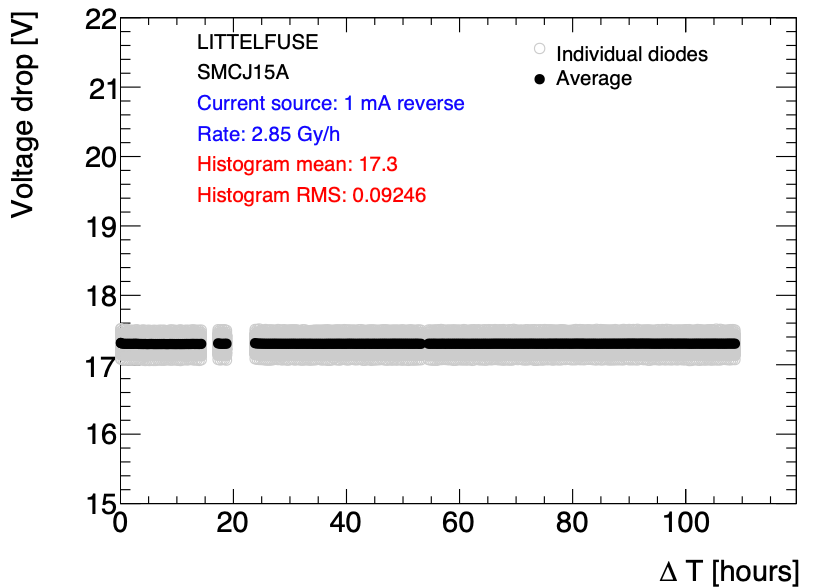
\includegraphics[width=0.8\linewidth]{assets/ATL-TILECAL-SLIDE-2025-552_slide_8_item_5.png}
\end{figure}

Seyedali Moayedi

Topical Workshop on Electronics for Particle Physics -- 8 October 2025

8

\section*{Slide 9}

\begin{figure}[H]
\centering

\includegraphics[width=0.8\linewidth]{assets/ATL-TILECAL-SLIDE-2025-552_slide_9_item_1.png}
\end{figure}

Radiation Tests: Diodes (2)

   For the rest of the diodes, the TID tests were performed by reverse  
biasing them during the beam time

   During the stop time, the relay board was used to go through the  
diode array and conduct a forward current and measure the forward  
voltage for each diode

   Performed at a flux of 3.6 Gy/h,  TID tests were successful

   All the diode boards were then annealed, and no significant change  
were observed in any of the them

   NIEL tests for all diodes showed no failure or change in parameters

\begin{figure}[H]
\centering
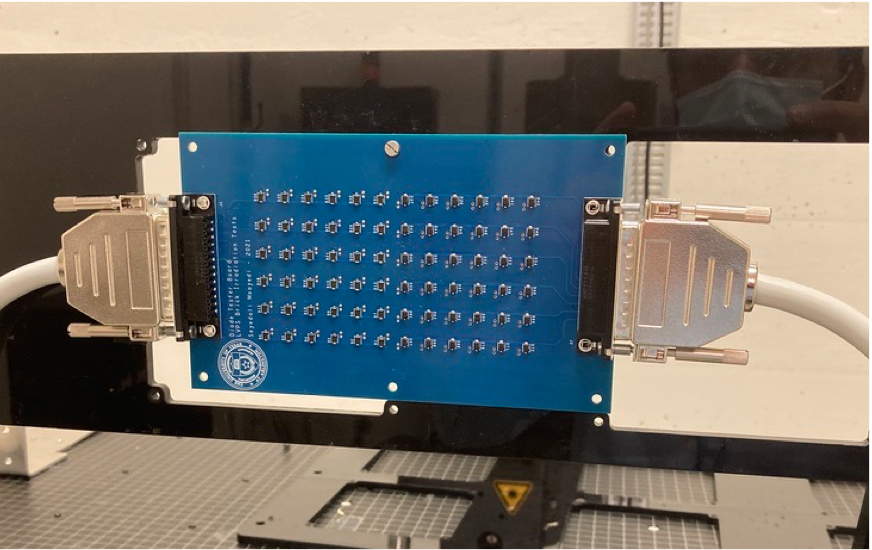
\includegraphics[width=0.8\linewidth]{assets/ATL-TILECAL-SLIDE-2025-552_slide_9_item_2.png}
\end{figure}

\begin{figure}[H]
\centering
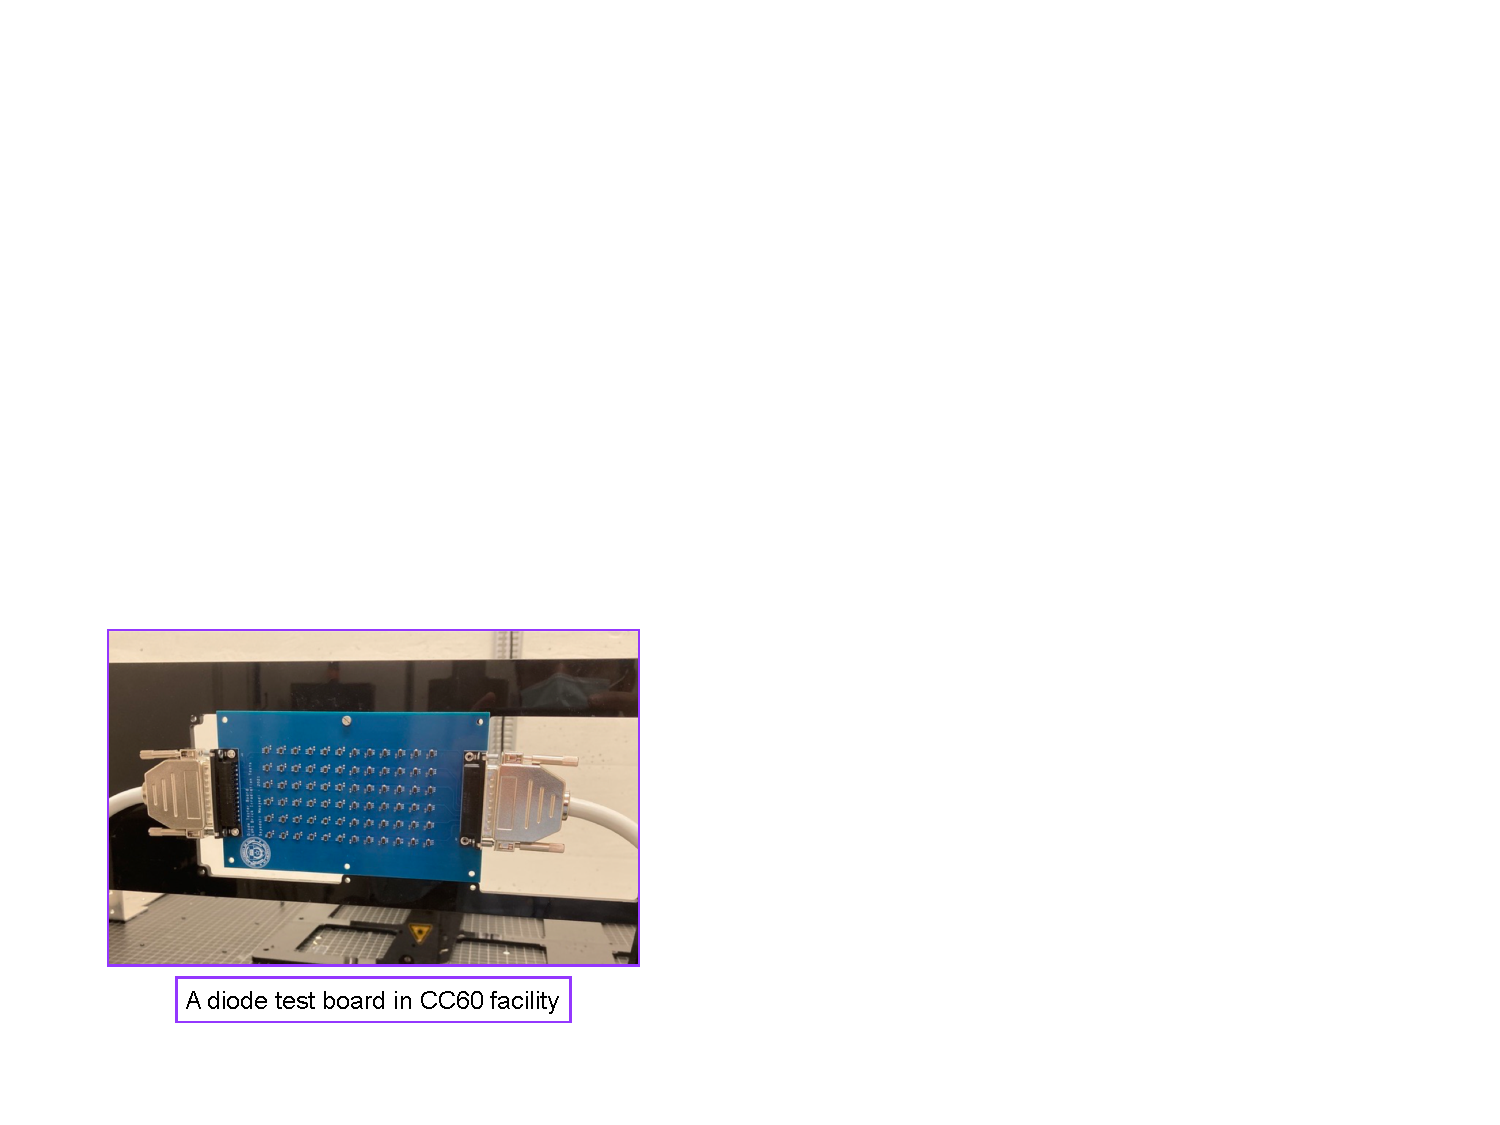
\includegraphics[width=0.8\linewidth]{assets/ATL-TILECAL-SLIDE-2025-552_slide_9_item_3.pdf}
\end{figure}

\begin{figure}[H]
\centering
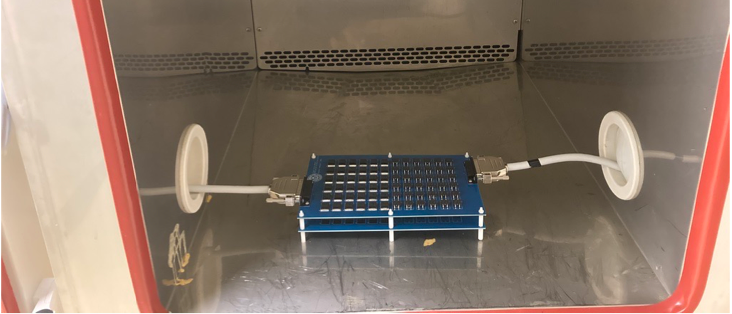
\includegraphics[width=0.8\linewidth]{assets/ATL-TILECAL-SLIDE-2025-552_slide_9_item_4.png}
\end{figure}

\begin{figure}[H]
\centering
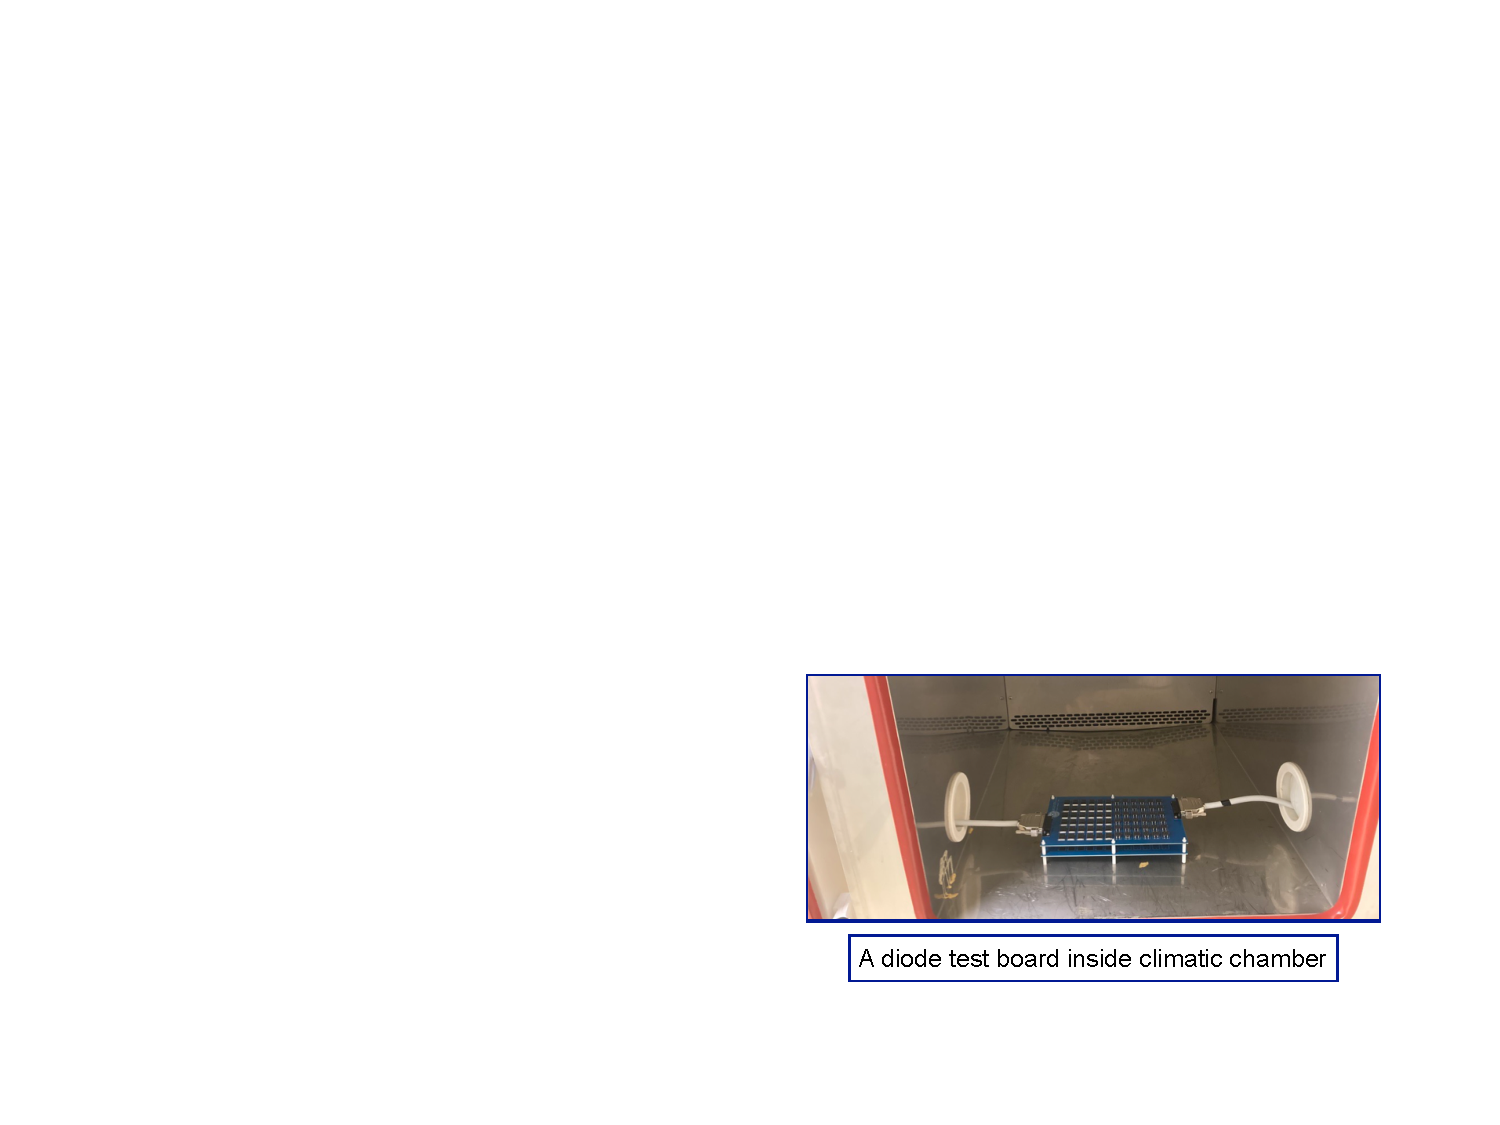
\includegraphics[width=0.8\linewidth]{assets/ATL-TILECAL-SLIDE-2025-552_slide_9_item_5.pdf}
\end{figure}

Seyedali Moayedi

Topical Workshop on Electronics for Particle Physics -- 8 October 2025

9

\section*{Slide 10}

\begin{figure}[H]
\centering

\includegraphics[width=0.8\linewidth]{assets/ATL-TILECAL-SLIDE-2025-552_slide_10_item_1.png}
\end{figure}

Radiation Tests: LT1681 Controller Chip

   TID and SEE tests performed together at a flux of 2.4 x 10 8  p/cm 2 /s

   Frequency of output pulses were monitored, as well as 1.25 V and 5 V  
reference voltages

   No change in frequencies happened and a maximum of 3\% drop in  
1.25 V reference voltages was seen (will cause 3\% brick voltage drop)

   The soft start pin was also being monitored for Single Event Upsets  
(SEUs), as there is an internal SR latch connected to this pin

   Few SEUs were observed, but due to external protection, transients  
were short, and they won't cause any trips in the bricks

   In overall,  the chips passed TID and SEE tests

   NIEL tests showed no issues

\begin{figure}[H]
\centering
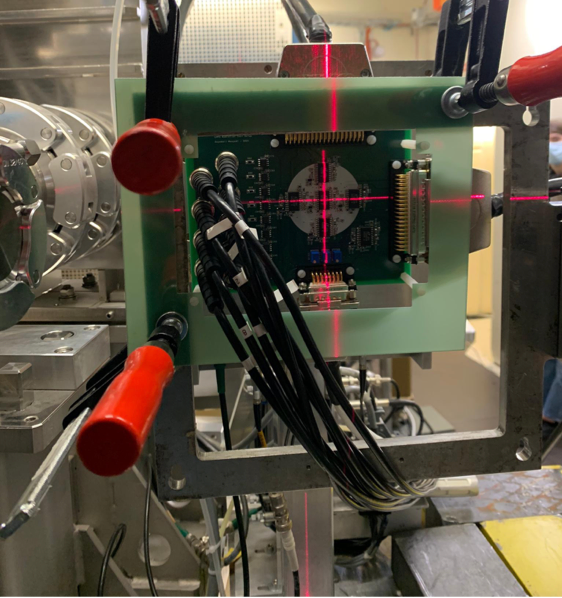
\includegraphics[width=0.8\linewidth]{assets/ATL-TILECAL-SLIDE-2025-552_slide_10_item_2.png}
\end{figure}

\begin{figure}[H]
\centering
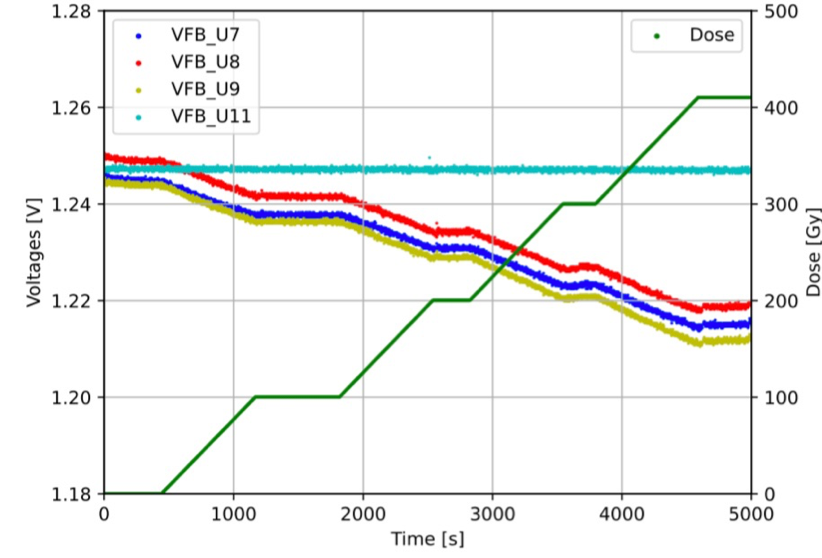
\includegraphics[width=0.8\linewidth]{assets/ATL-TILECAL-SLIDE-2025-552_slide_10_item_3.png}
\end{figure}

\begin{figure}[H]
\centering
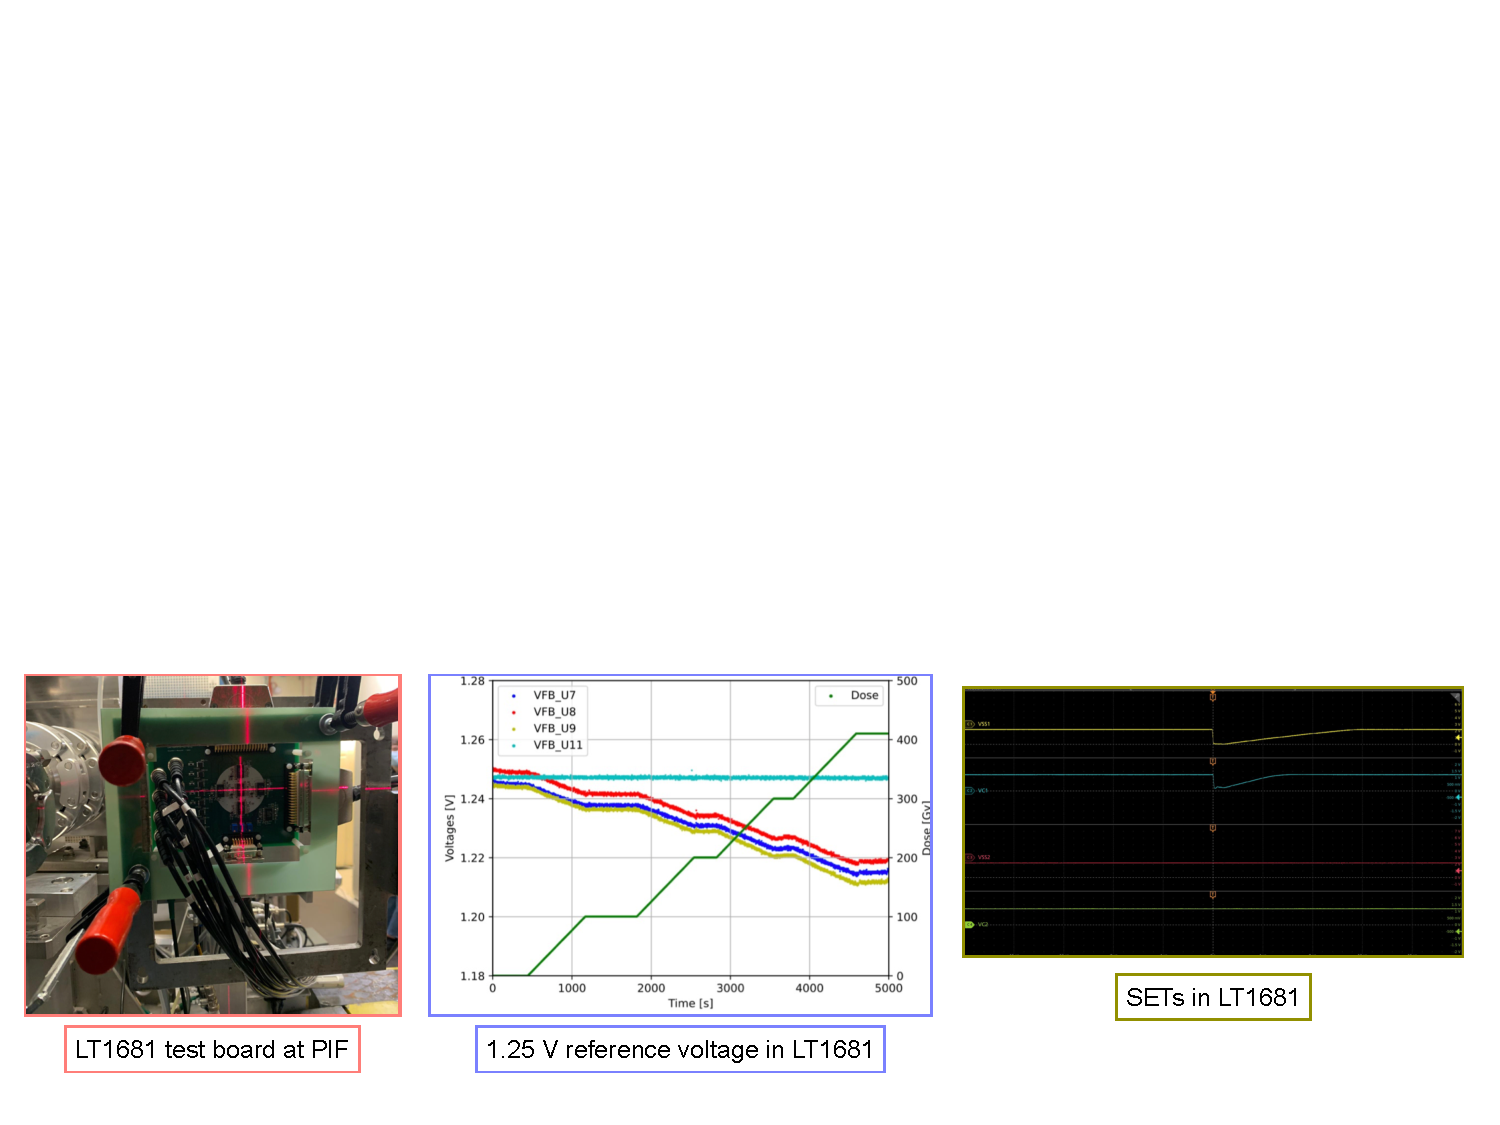
\includegraphics[width=0.8\linewidth]{assets/ATL-TILECAL-SLIDE-2025-552_slide_10_item_4.pdf}
\end{figure}

\begin{figure}[H]
\centering
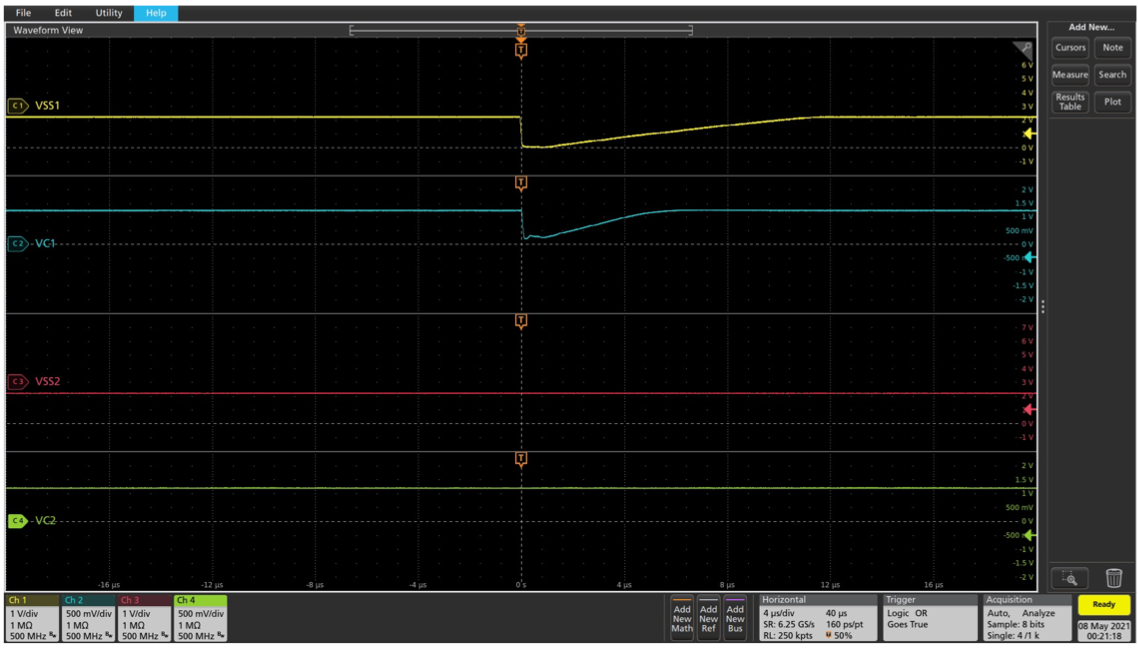
\includegraphics[width=0.8\linewidth]{assets/ATL-TILECAL-SLIDE-2025-552_slide_10_item_5.png}
\end{figure}

Seyedali Moayedi

Topical Workshop on Electronics for Particle Physics -- 8 October 2025

10

\section*{Slide 11}

\begin{figure}[H]
\centering

\includegraphics[width=0.8\linewidth]{assets/ATL-TILECAL-SLIDE-2025-552_slide_11_item_1.png}
\end{figure}

Radiation Tests: LTC6241 Op-Amp

   SEE tests performed at a flux of 2.4 x 10 8  p/cm 2 /s

   The monitored parameters were bias current, offset voltage, output  
voltage drift, and Single Event Transients (SET) on output voltages

   No significant change was observed in parameters

   Some SETs were observed, with small amplitude (\textasciitilde{}50 mV) and short  
duration (\textasciitilde{}100 ns), but they have no effect on brick's performance

   The chips passed the SEE tests successfully

   Performed at 3 Gy/h followed by annealing,  TID tests showed no  
significant change in parameters

   NIEL tests showed no change in parameters

\begin{figure}[H]
\centering
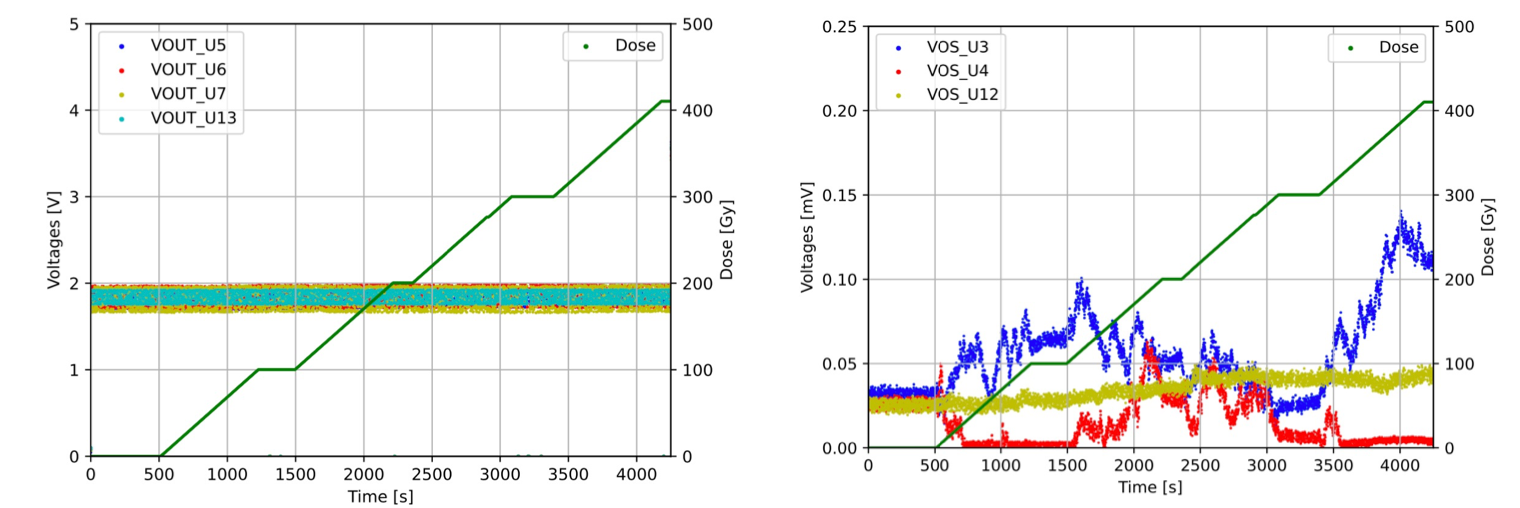
\includegraphics[width=0.8\linewidth]{assets/ATL-TILECAL-SLIDE-2025-552_slide_11_item_2.png}
\end{figure}

\begin{figure}[H]
\centering
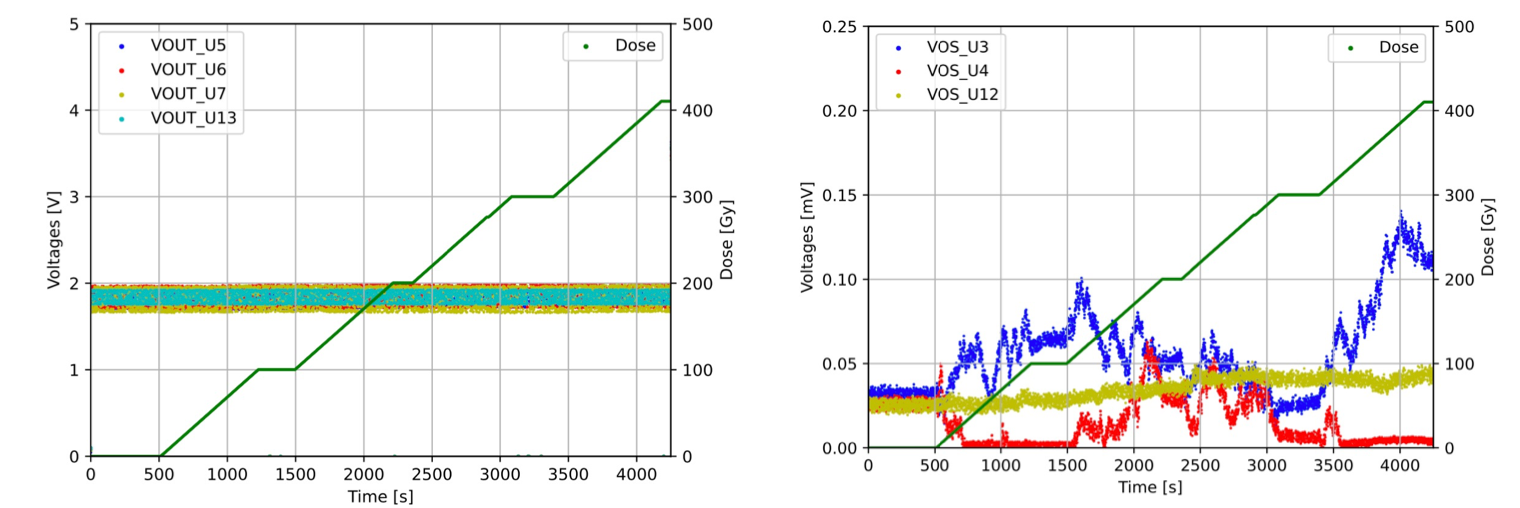
\includegraphics[width=0.8\linewidth]{assets/ATL-TILECAL-SLIDE-2025-552_slide_11_item_3.png}
\end{figure}

\begin{figure}[H]
\centering
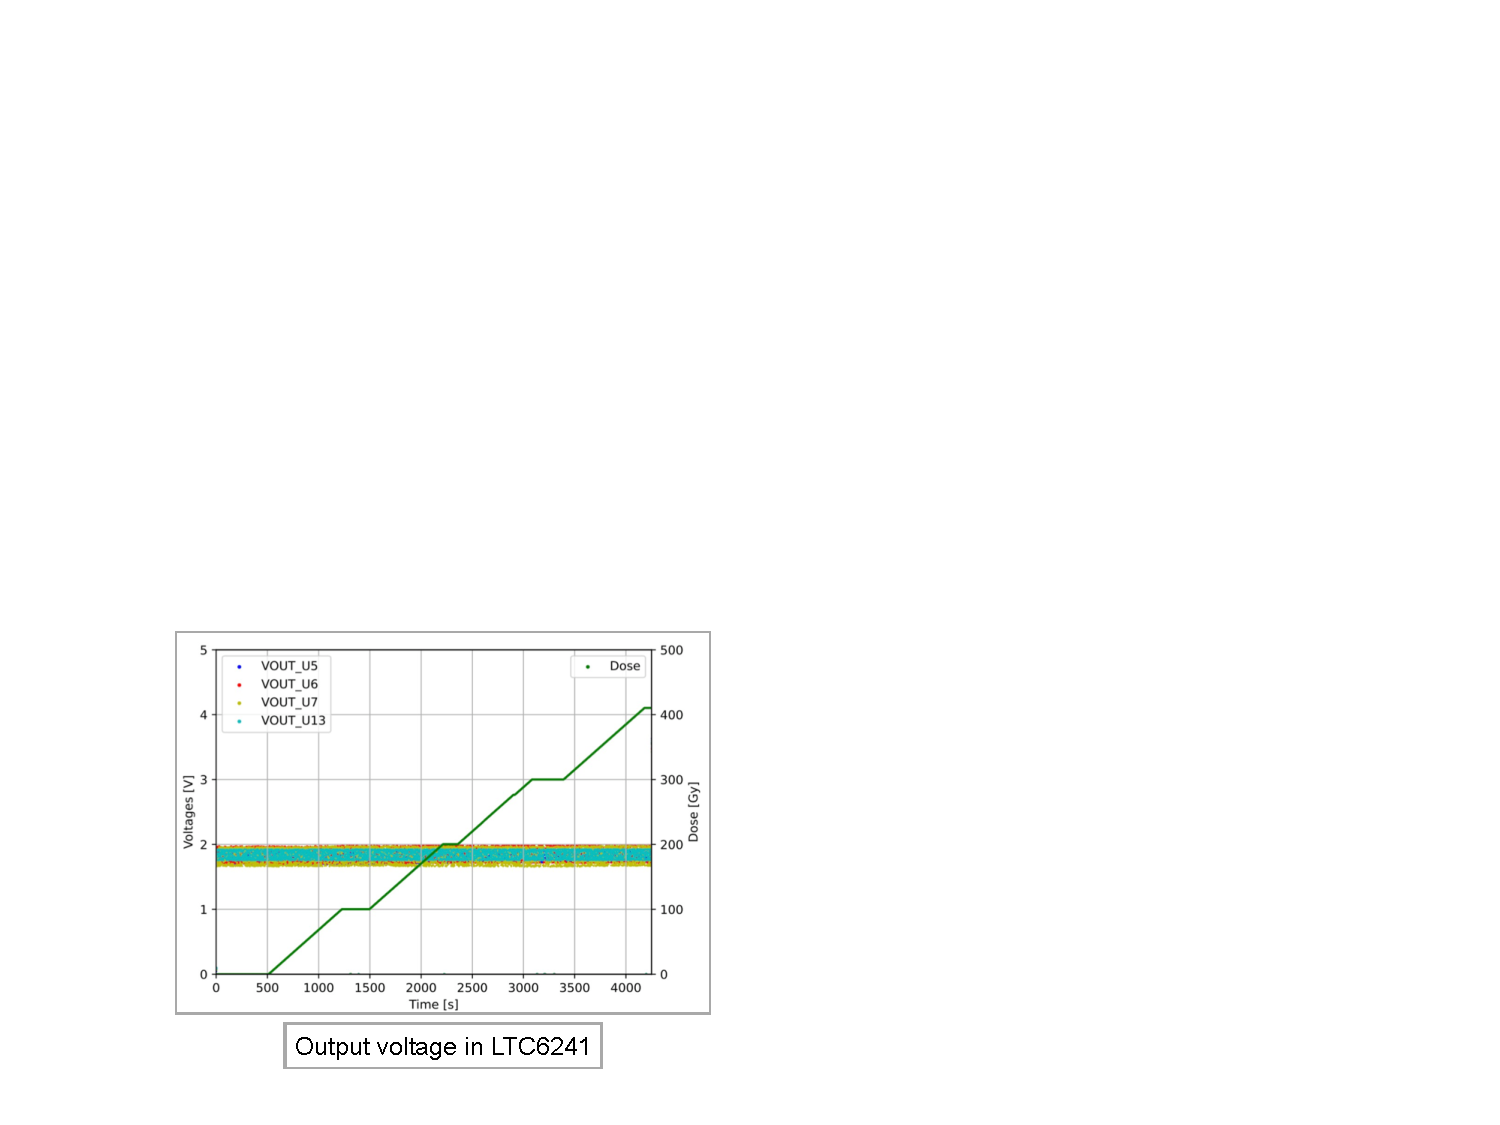
\includegraphics[width=0.8\linewidth]{assets/ATL-TILECAL-SLIDE-2025-552_slide_11_item_4.pdf}
\end{figure}

\begin{figure}[H]
\centering
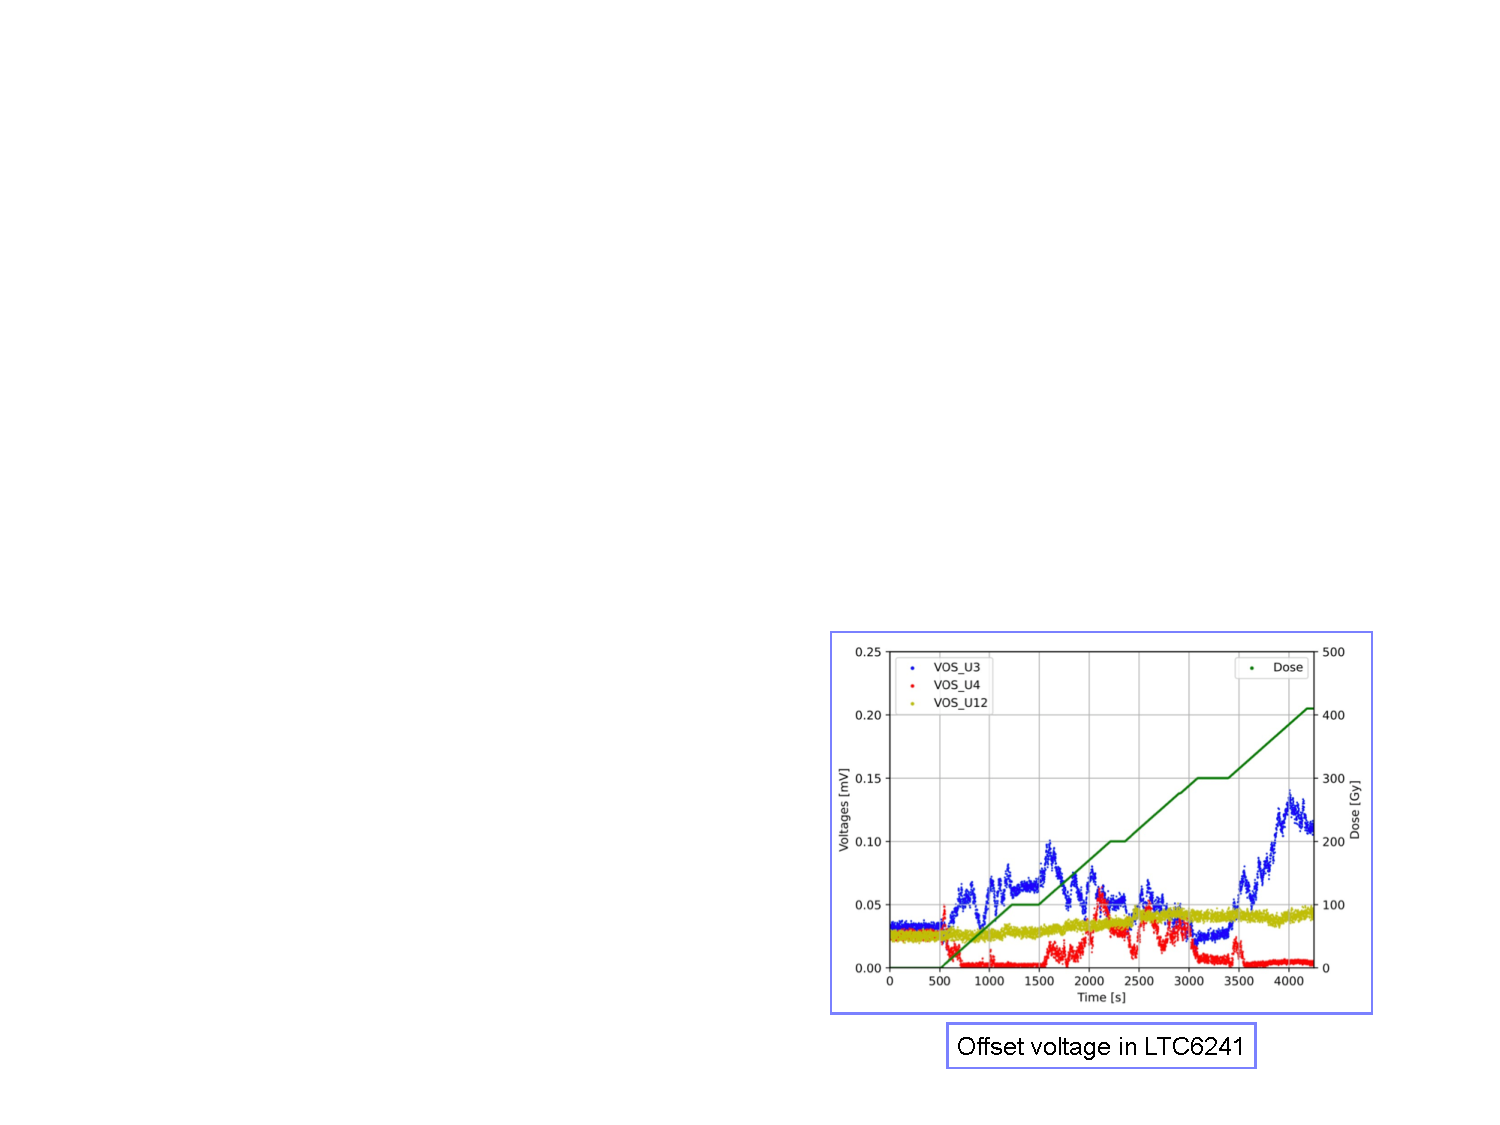
\includegraphics[width=0.8\linewidth]{assets/ATL-TILECAL-SLIDE-2025-552_slide_11_item_5.pdf}
\end{figure}

Seyedali Moayedi

Topical Workshop on Electronics for Particle Physics -- 8 October 2025

11

\section*{Slide 12}

\begin{figure}[H]
\centering

\includegraphics[width=0.8\linewidth]{assets/ATL-TILECAL-SLIDE-2025-552_slide_12_item_1.png}
\end{figure}

Radiation Tests: LT3080 Voltage Regulator

   TID and SEE tests performed together at a flux of 2.4 x 10 8  p/cm 2 /s

   Output voltages of the chips were being monitored

   A maximum of 5\% increase in output voltages were observed (no effect on  
brick's performance)

   Some SETs were observed, with small amplitude (max 500 mV) and short  
duration (\textasciitilde{}20 us), but with no effect on brick's performance

   NIEL tests showed no issues

   As failures on this chip were observed by other groups at CHARM facility, it  
was asked to retest these chips at a mixed field

   Tests at CHARM showed no failures  up to 835 Gy and 6.57 x 10 12  n/cm 2

\begin{figure}[H]
\centering
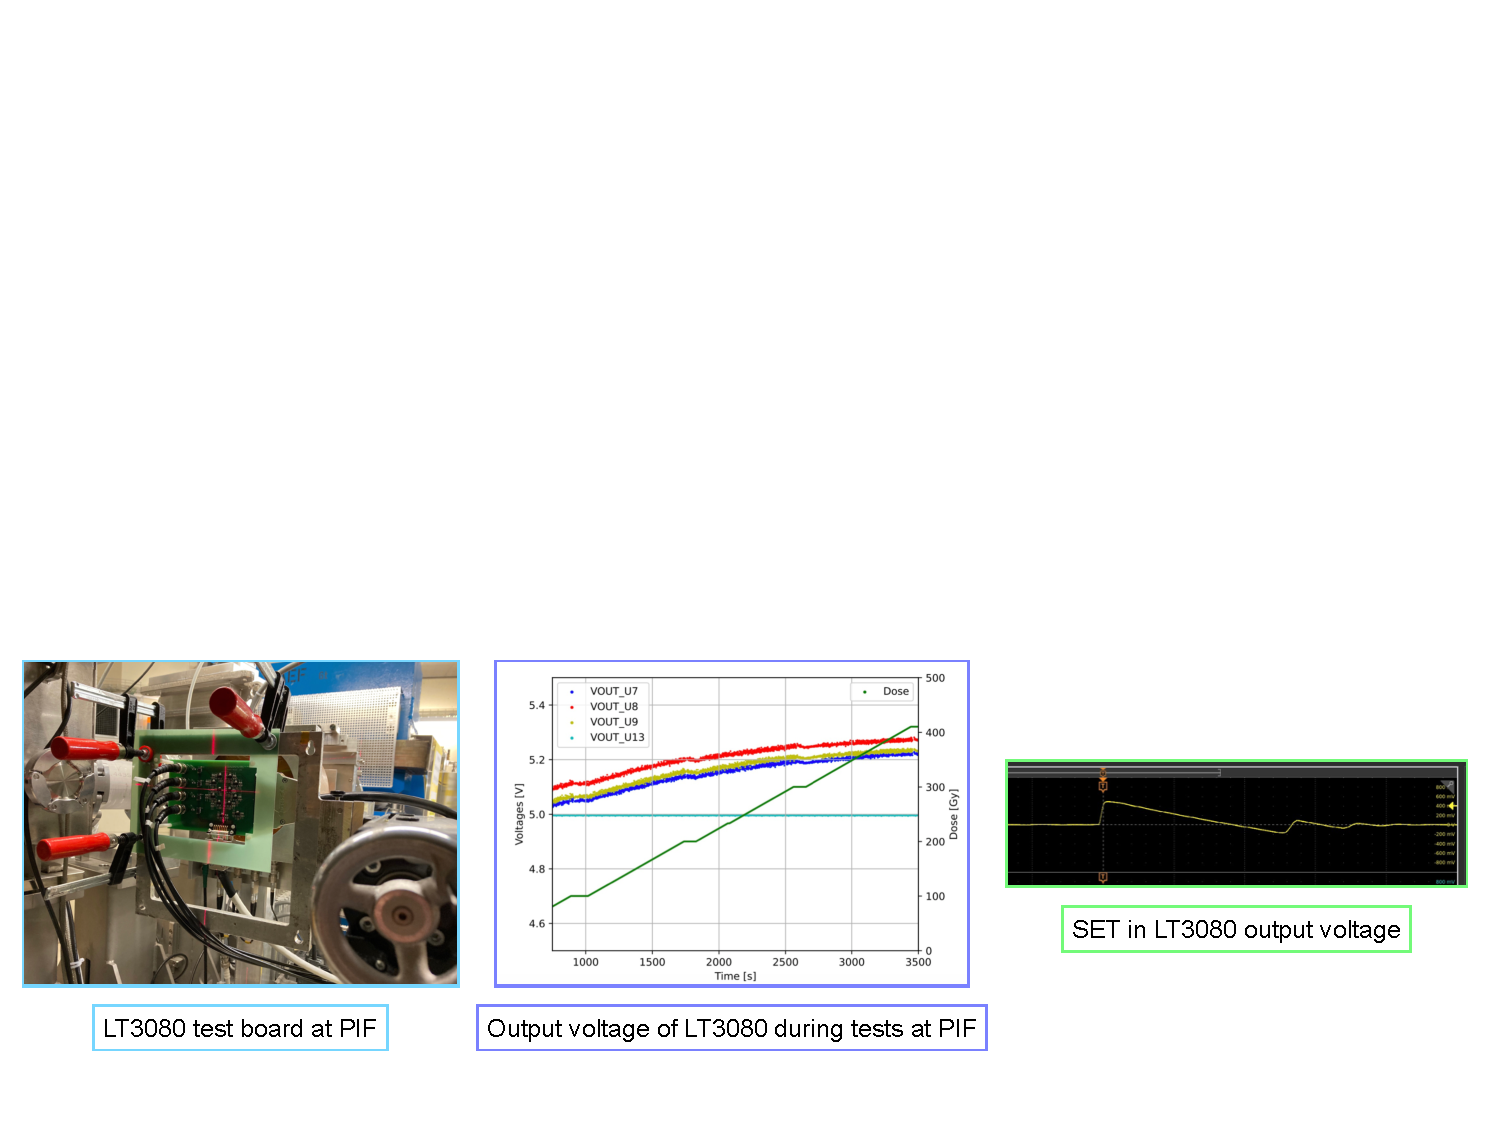
\includegraphics[width=0.8\linewidth]{assets/ATL-TILECAL-SLIDE-2025-552_slide_12_item_2.pdf}
\end{figure}

\begin{figure}[H]
\centering
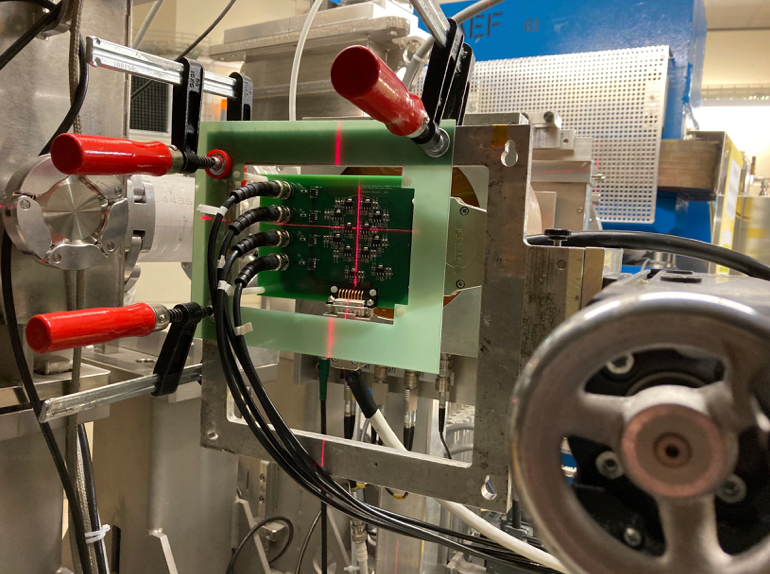
\includegraphics[width=0.8\linewidth]{assets/ATL-TILECAL-SLIDE-2025-552_slide_12_item_3.png}
\end{figure}

\begin{figure}[H]
\centering
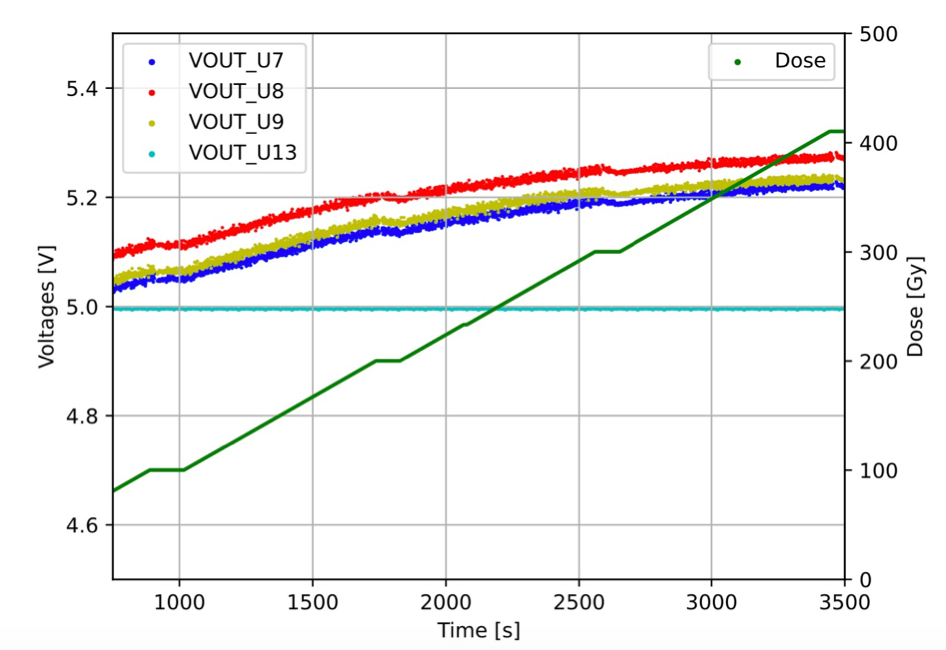
\includegraphics[width=0.8\linewidth]{assets/ATL-TILECAL-SLIDE-2025-552_slide_12_item_4.png}
\end{figure}

\begin{figure}[H]
\centering
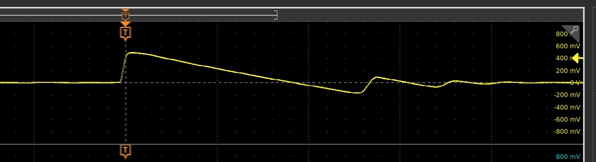
\includegraphics[width=0.8\linewidth]{assets/ATL-TILECAL-SLIDE-2025-552_slide_12_item_5.png}
\end{figure}

Seyedali Moayedi

Topical Workshop on Electronics for Particle Physics -- 8 October 2025

12

\section*{Slide 13}

\begin{figure}[H]
\centering

\includegraphics[width=0.8\linewidth]{assets/ATL-TILECAL-SLIDE-2025-552_slide_13_item_1.png}
\end{figure}

Radiation Tests: IR2110 MOSFET Driver

   SEE tests performed at a flux of 3.5 x 10 8  p/cm 2 /s

   Output pulses for 8 chips, set on 300 kHz, were monitored

   There was no significant changes to the pulse shapes during the tests

   Two chips were monitored for SEEs and no events were observed up to  
3.4 x 10 11  p/cm 2 ,  passing the SEE tests

   Performed at 3 Gy/h up followed by annealing,  TID tests showed no  
significant change in parameters

   The chips tested for NIEL showed no issues

\begin{figure}[H]
\centering
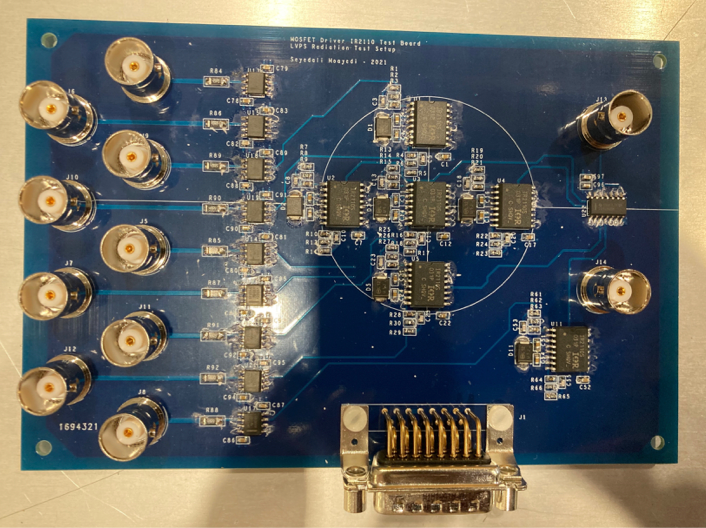
\includegraphics[width=0.8\linewidth]{assets/ATL-TILECAL-SLIDE-2025-552_slide_13_item_2.png}
\end{figure}

\begin{figure}[H]
\centering
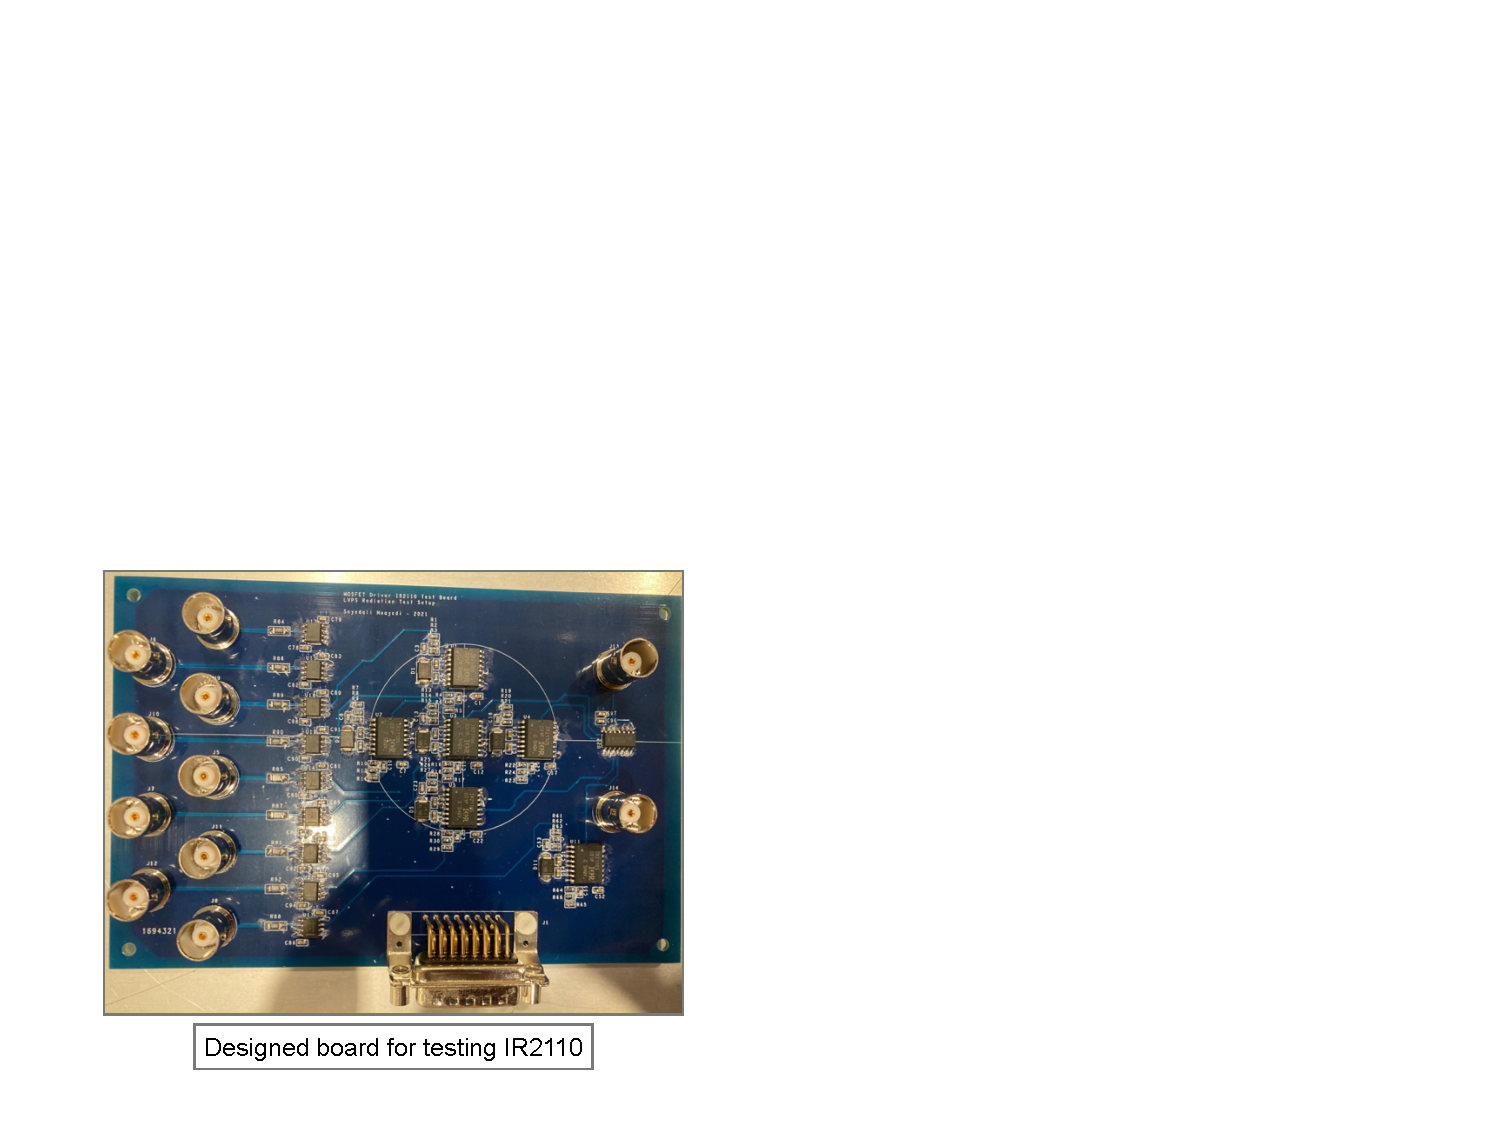
\includegraphics[width=0.8\linewidth]{assets/ATL-TILECAL-SLIDE-2025-552_slide_13_item_3.pdf}
\end{figure}

\begin{figure}[H]
\centering
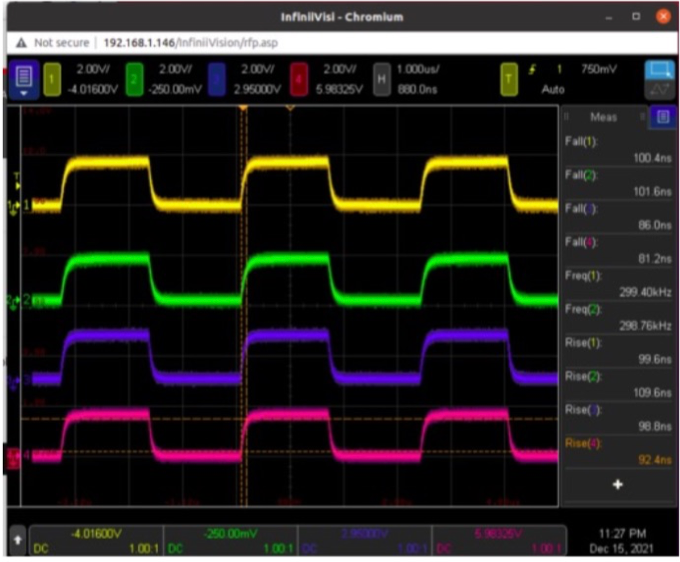
\includegraphics[width=0.8\linewidth]{assets/ATL-TILECAL-SLIDE-2025-552_slide_13_item_4.png}
\end{figure}

\begin{figure}[H]
\centering
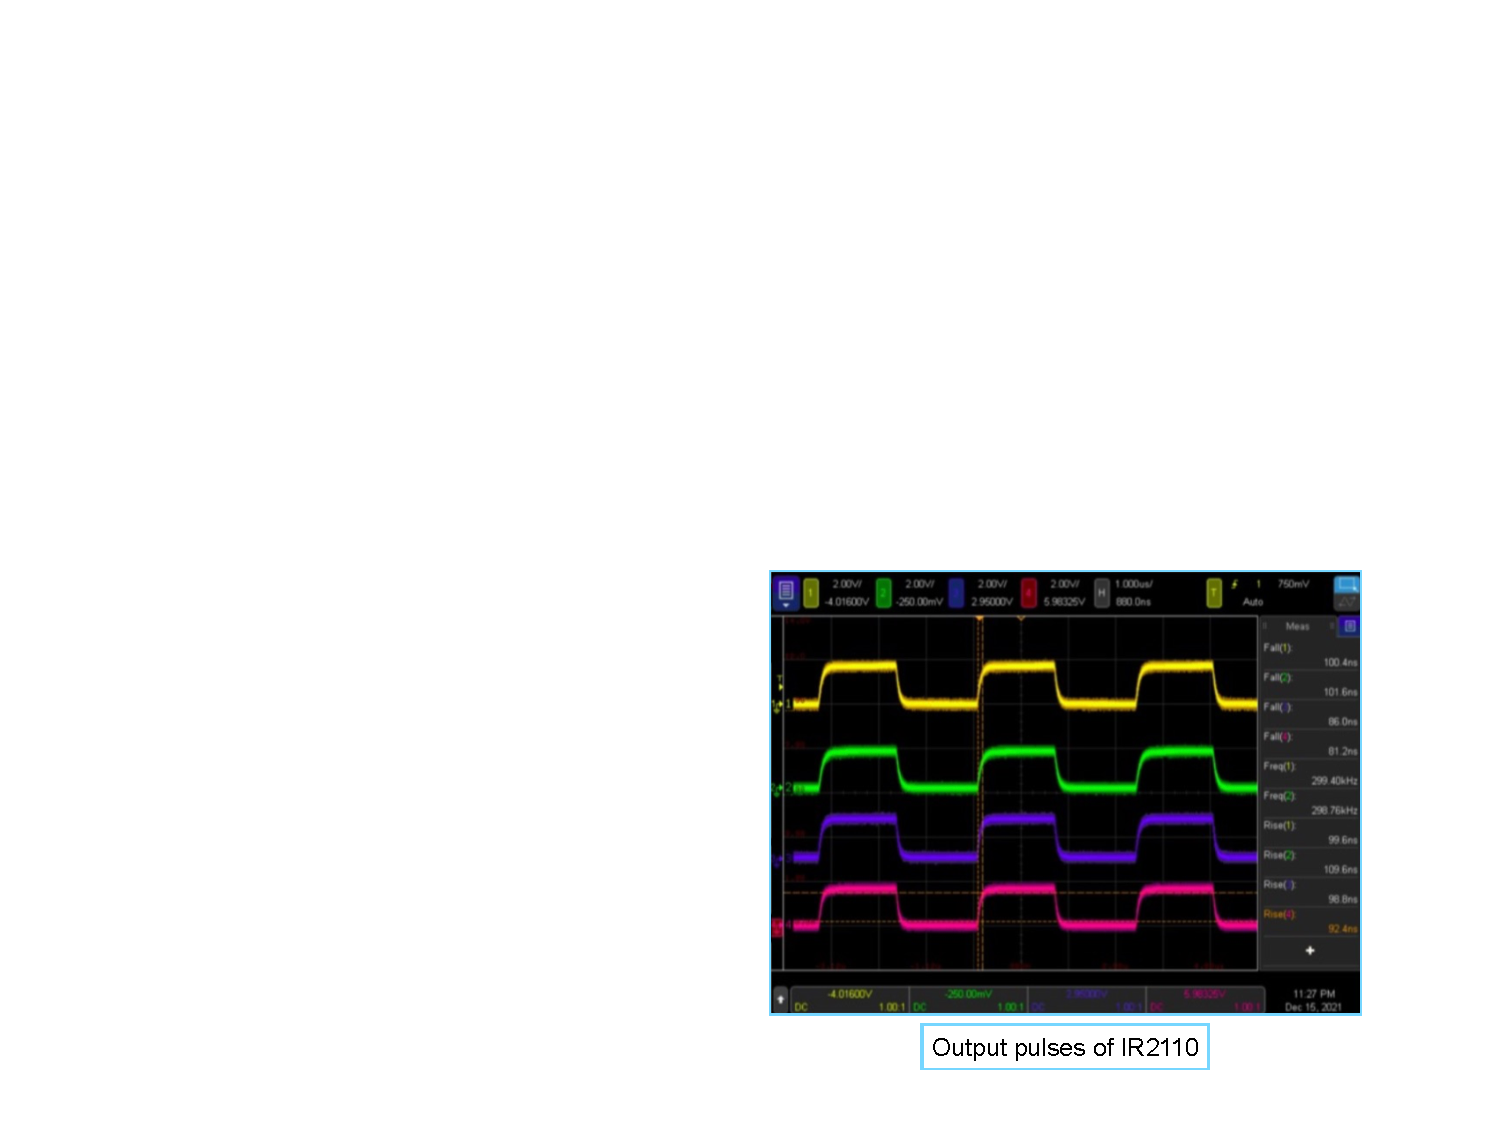
\includegraphics[width=0.8\linewidth]{assets/ATL-TILECAL-SLIDE-2025-552_slide_13_item_5.pdf}
\end{figure}

Seyedali Moayedi

Topical Workshop on Electronics for Particle Physics -- 8 October 2025

13

\section*{Slide 14}

\begin{figure}[H]
\centering

\includegraphics[width=0.8\linewidth]{assets/ATL-TILECAL-SLIDE-2025-552_slide_14_item_1.png}
\end{figure}

Radiation Tests: SIHFS9N60A MOSFET

   SEE tests performed at a flux of 3.5 x 10 8  p/cm 2 /s

   The chips were biased and monitored for SEEs, and no events  
observed up to 3.4 x 10 11  p/cm 2 ),  passing the SEE tests

   The chips were characterized at CERN after irradiation and a shift of  
2.5 V were observed in gate-source threshold voltage after 200 Gy (a  
very small effect in brick's performance)

   Performed at 3 Gy/h followed by annealing,  TID tests showed a  
smaller shift in gate-source threshold voltage, and were passed

   NIEL tests showed very small deviation in characterization  (due      
to gamma radiation in reactor)

\begin{figure}[H]
\centering
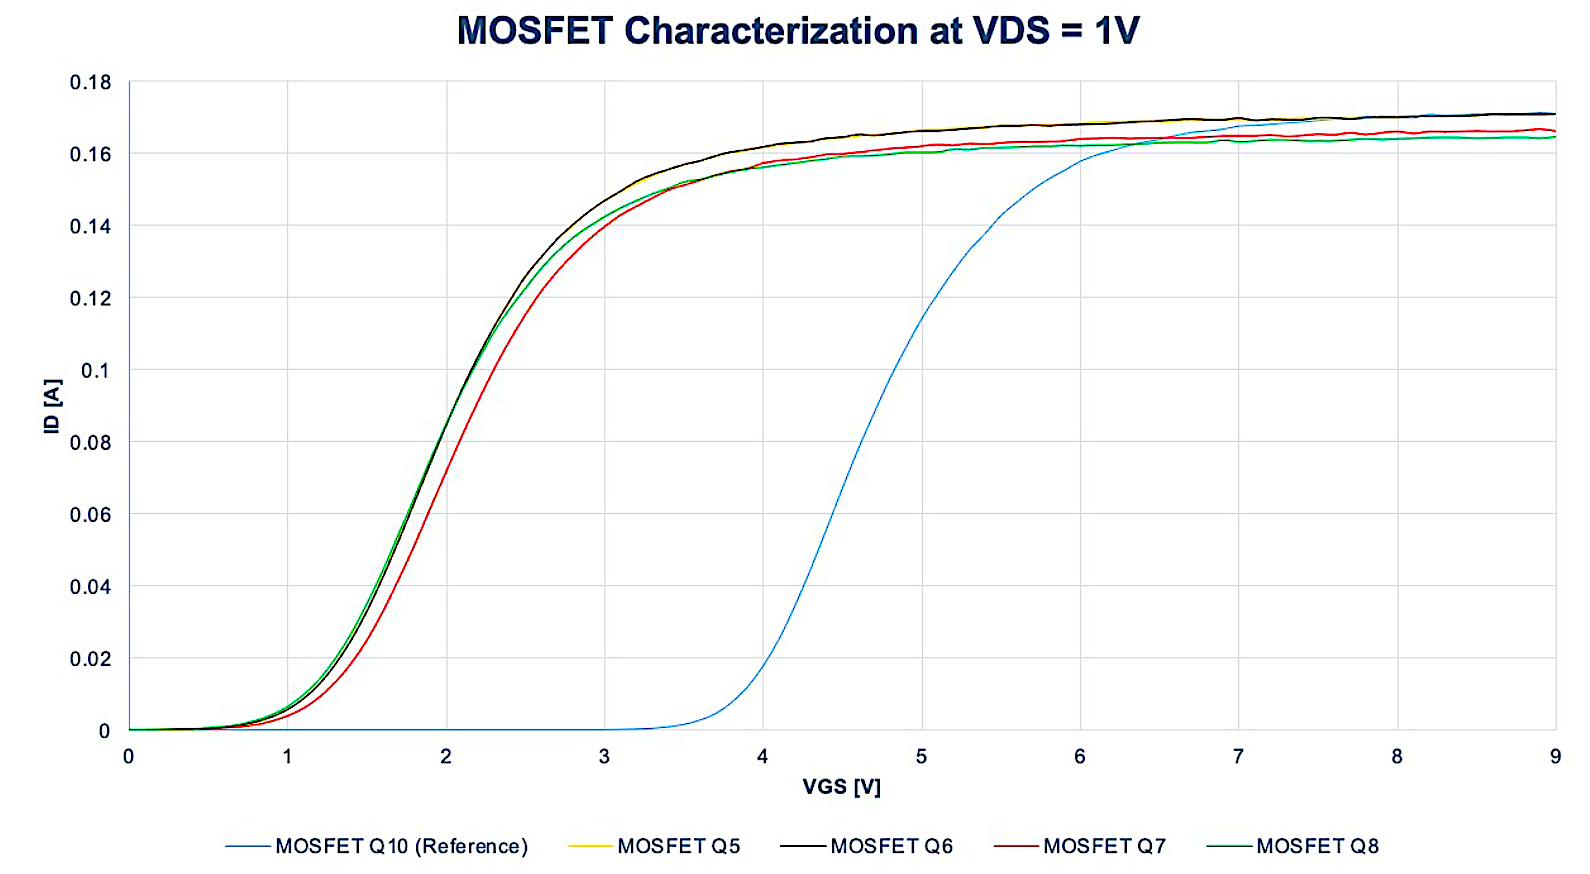
\includegraphics[width=0.8\linewidth]{assets/ATL-TILECAL-SLIDE-2025-552_slide_14_item_2.png}
\end{figure}

\begin{figure}[H]
\centering
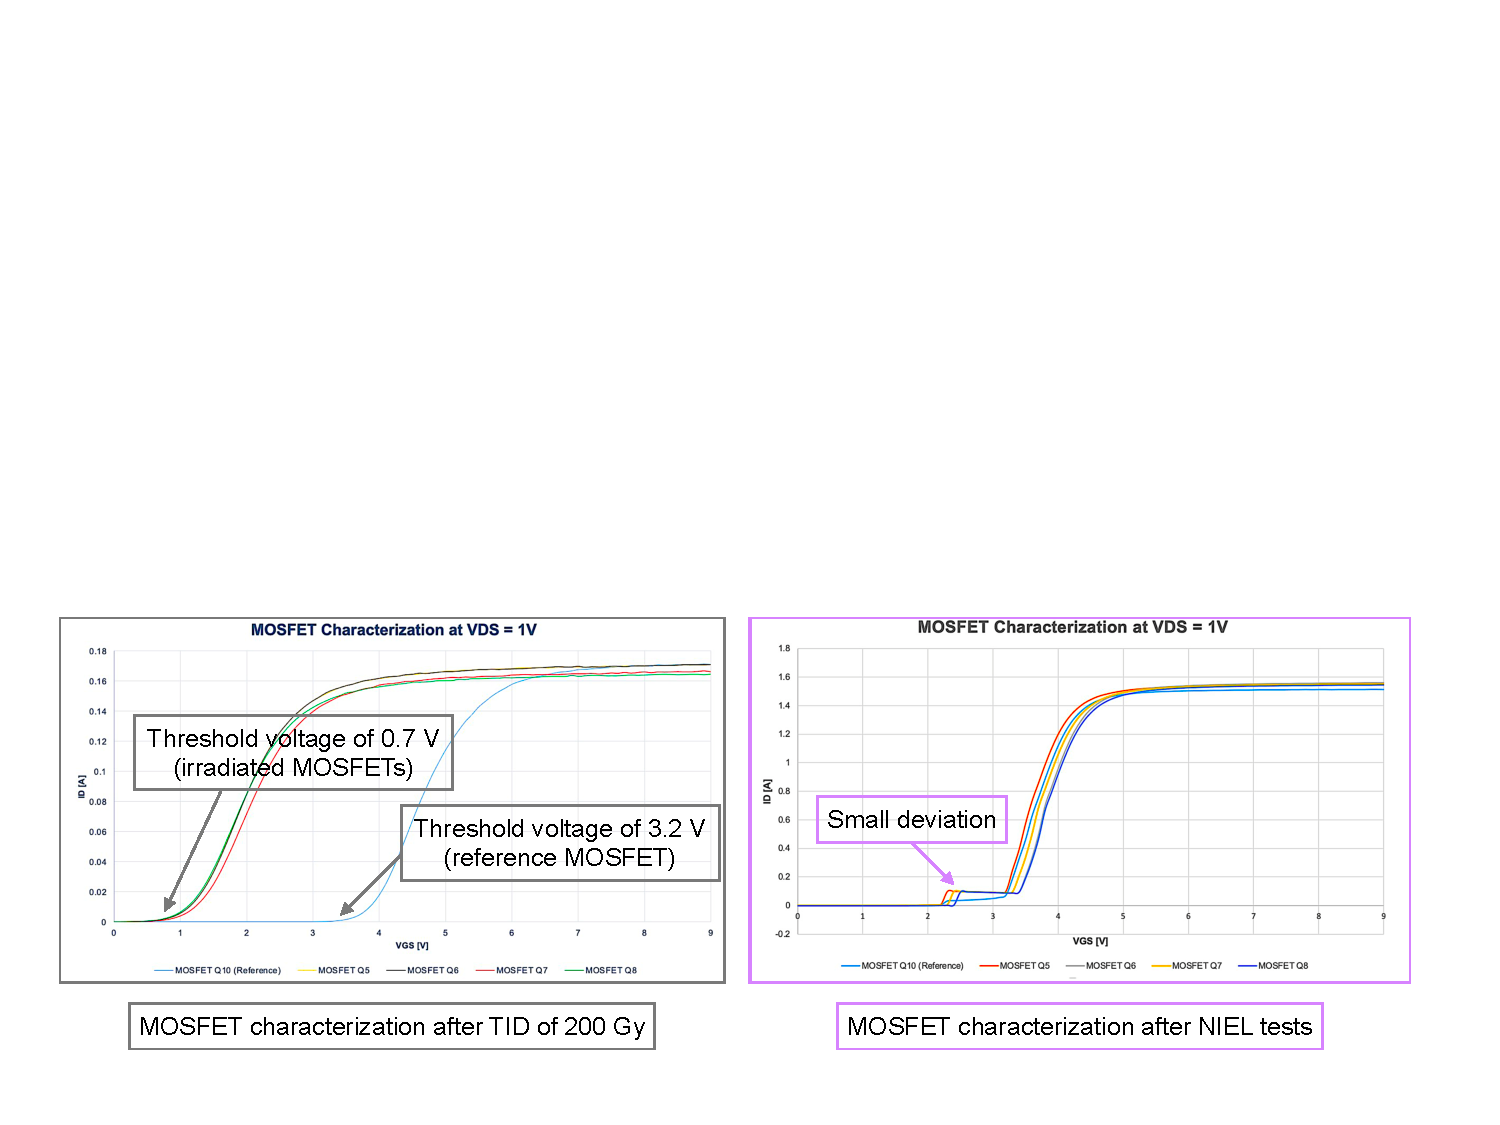
\includegraphics[width=0.8\linewidth]{assets/ATL-TILECAL-SLIDE-2025-552_slide_14_item_3.pdf}
\end{figure}

\begin{figure}[H]
\centering
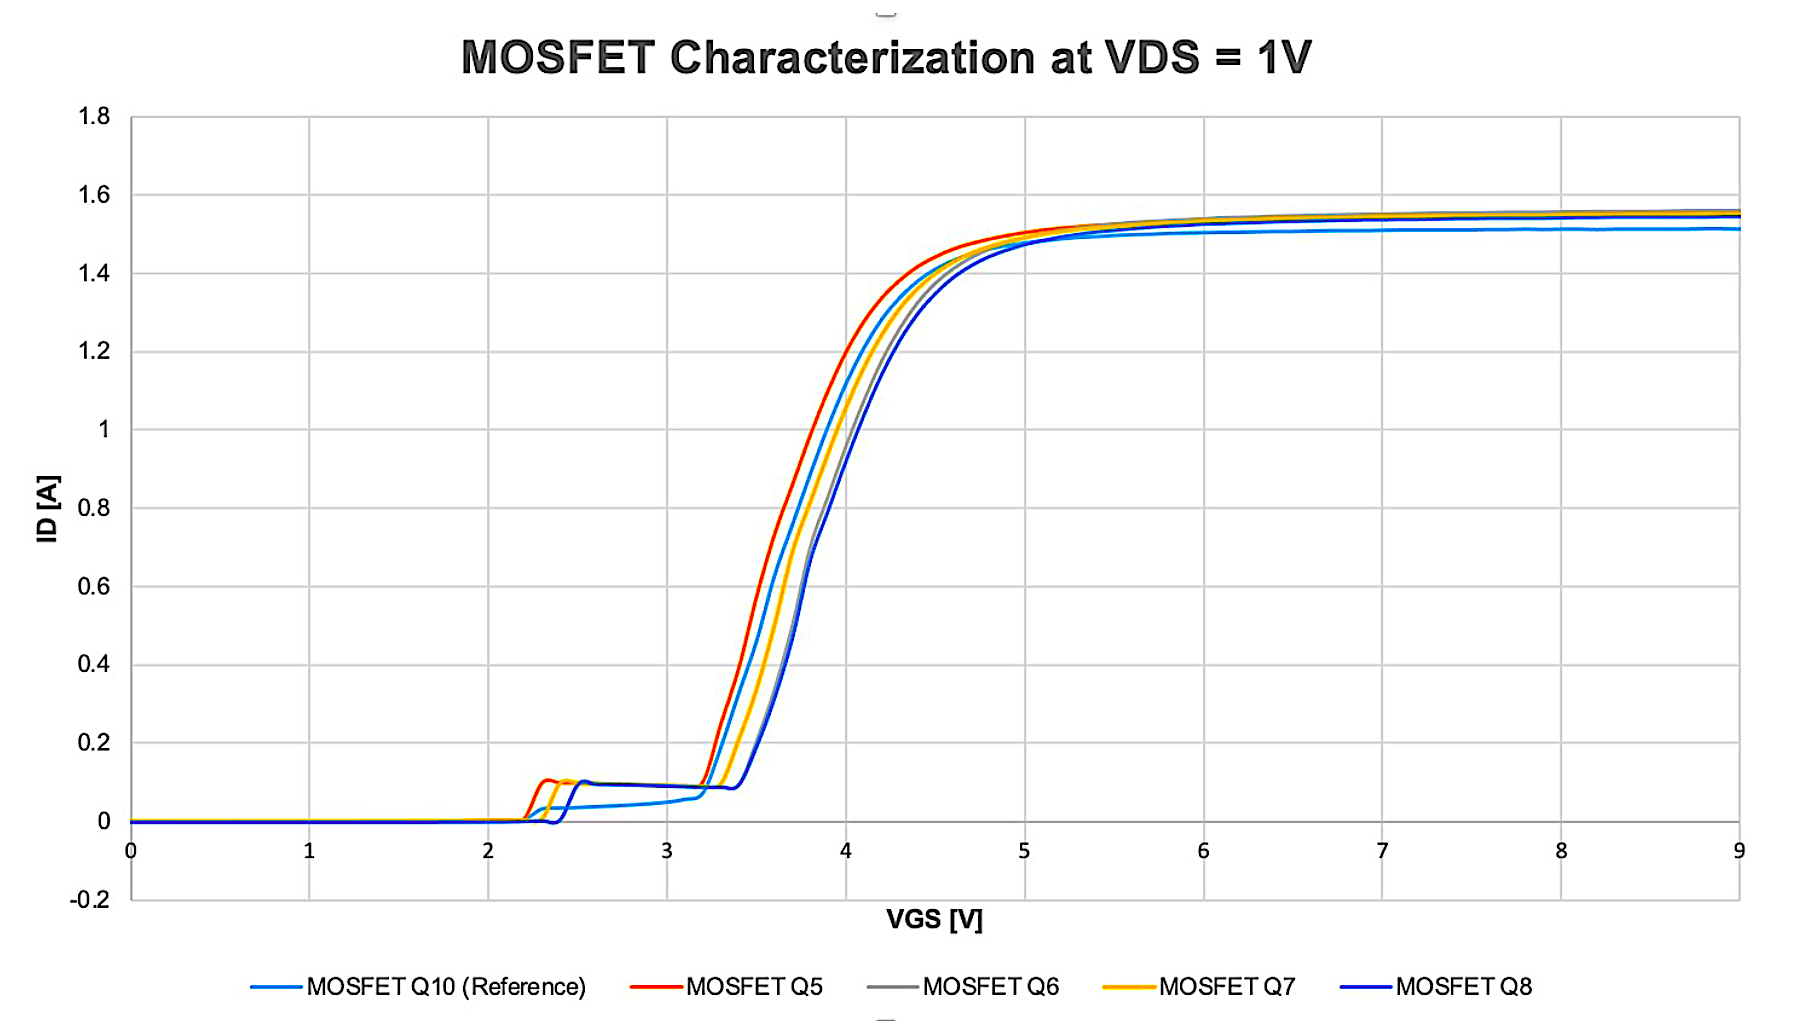
\includegraphics[width=0.8\linewidth]{assets/ATL-TILECAL-SLIDE-2025-552_slide_14_item_4.png}
\end{figure}

Seyedali Moayedi

Topical Workshop on Electronics for Particle Physics -- 8 October 2025

14

\section*{Slide 15}

\begin{figure}[H]
\centering

\includegraphics[width=0.8\linewidth]{assets/ATL-TILECAL-SLIDE-2025-552_slide_15_item_1.png}
\end{figure}

Radiation Tests: SI8920 Isolation Amplifier (1)

   Chips tested for NIEL showed no issues

   SEE/TID tests performed at a flux of 3.5 x 10 8  p/cm 2 /s

   With an input voltage of 150 mV, test results showed fluctuations in the  
output voltage of some chips during the beam time

   Another set of SEE/TID tests performed at a flux of 2 x 10 8  p/cm 2 /s, but  
the same behavior were observed

\begin{figure}[H]
\centering
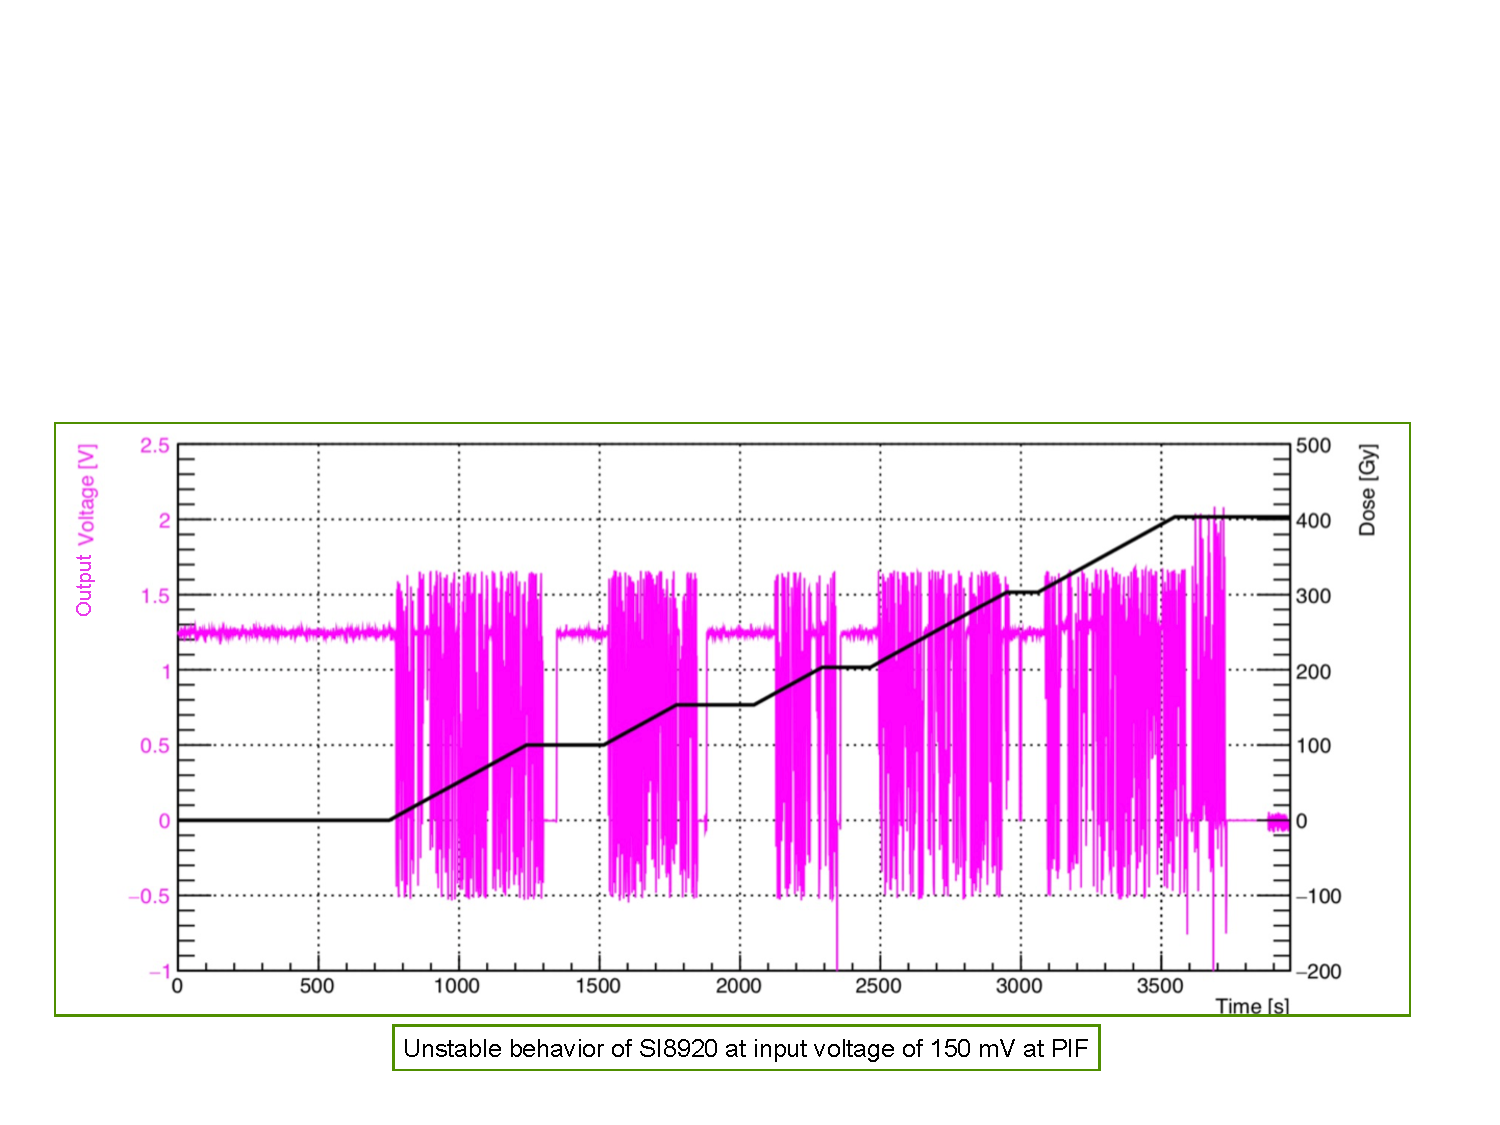
\includegraphics[width=0.8\linewidth]{assets/ATL-TILECAL-SLIDE-2025-552_slide_15_item_2.pdf}
\end{figure}

\begin{figure}[H]
\centering
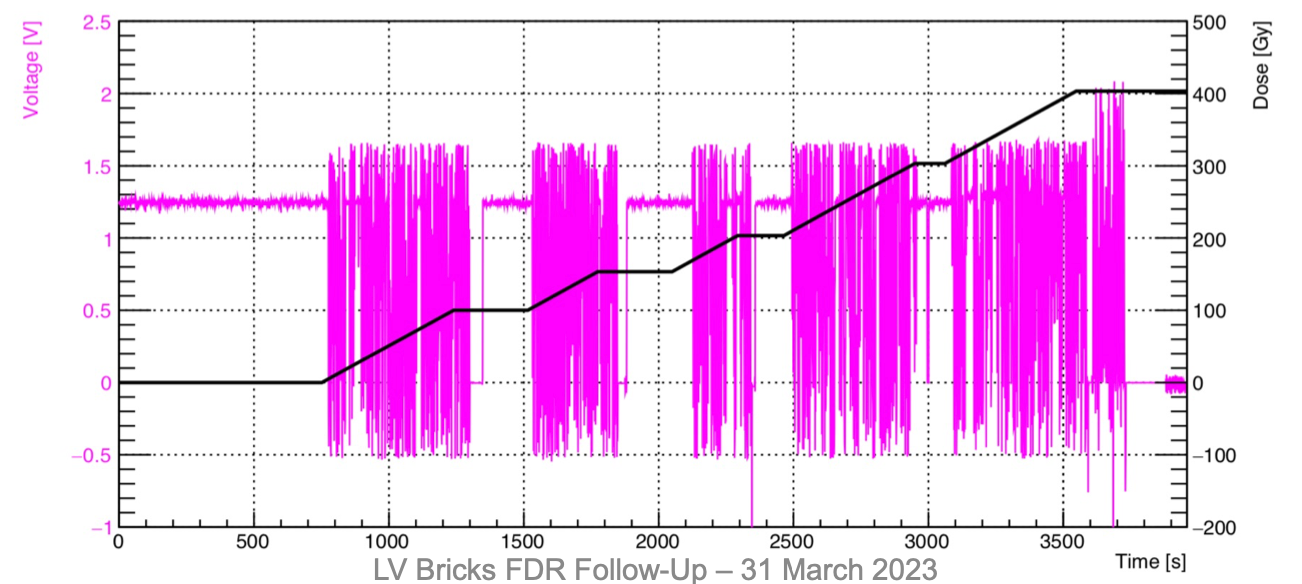
\includegraphics[width=0.8\linewidth]{assets/ATL-TILECAL-SLIDE-2025-552_slide_15_item_3.png}
\end{figure}

Seyedali Moayedi

Topical Workshop on Electronics for Particle Physics -- 8 October 2025

15

\section*{Slide 16}

\begin{figure}[H]
\centering

\includegraphics[width=0.8\linewidth]{assets/ATL-TILECAL-SLIDE-2025-552_slide_16_item_1.png}
\end{figure}

Radiation Tests: SI8920 Isolation Amplifier (2)

   After further tests at CHARM and PSI, we found that the chip has a  
stable behavior at a specific voltage range

   Having an input voltage below 100 mV,  the chip passed SEE and  
TID tests

   It was decided to use SI8920 for the production bricks, and ensuring  
that the circuits only allow the input voltage of this chip to be a maximum  
of 100 mV

\begin{figure}[H]
\centering
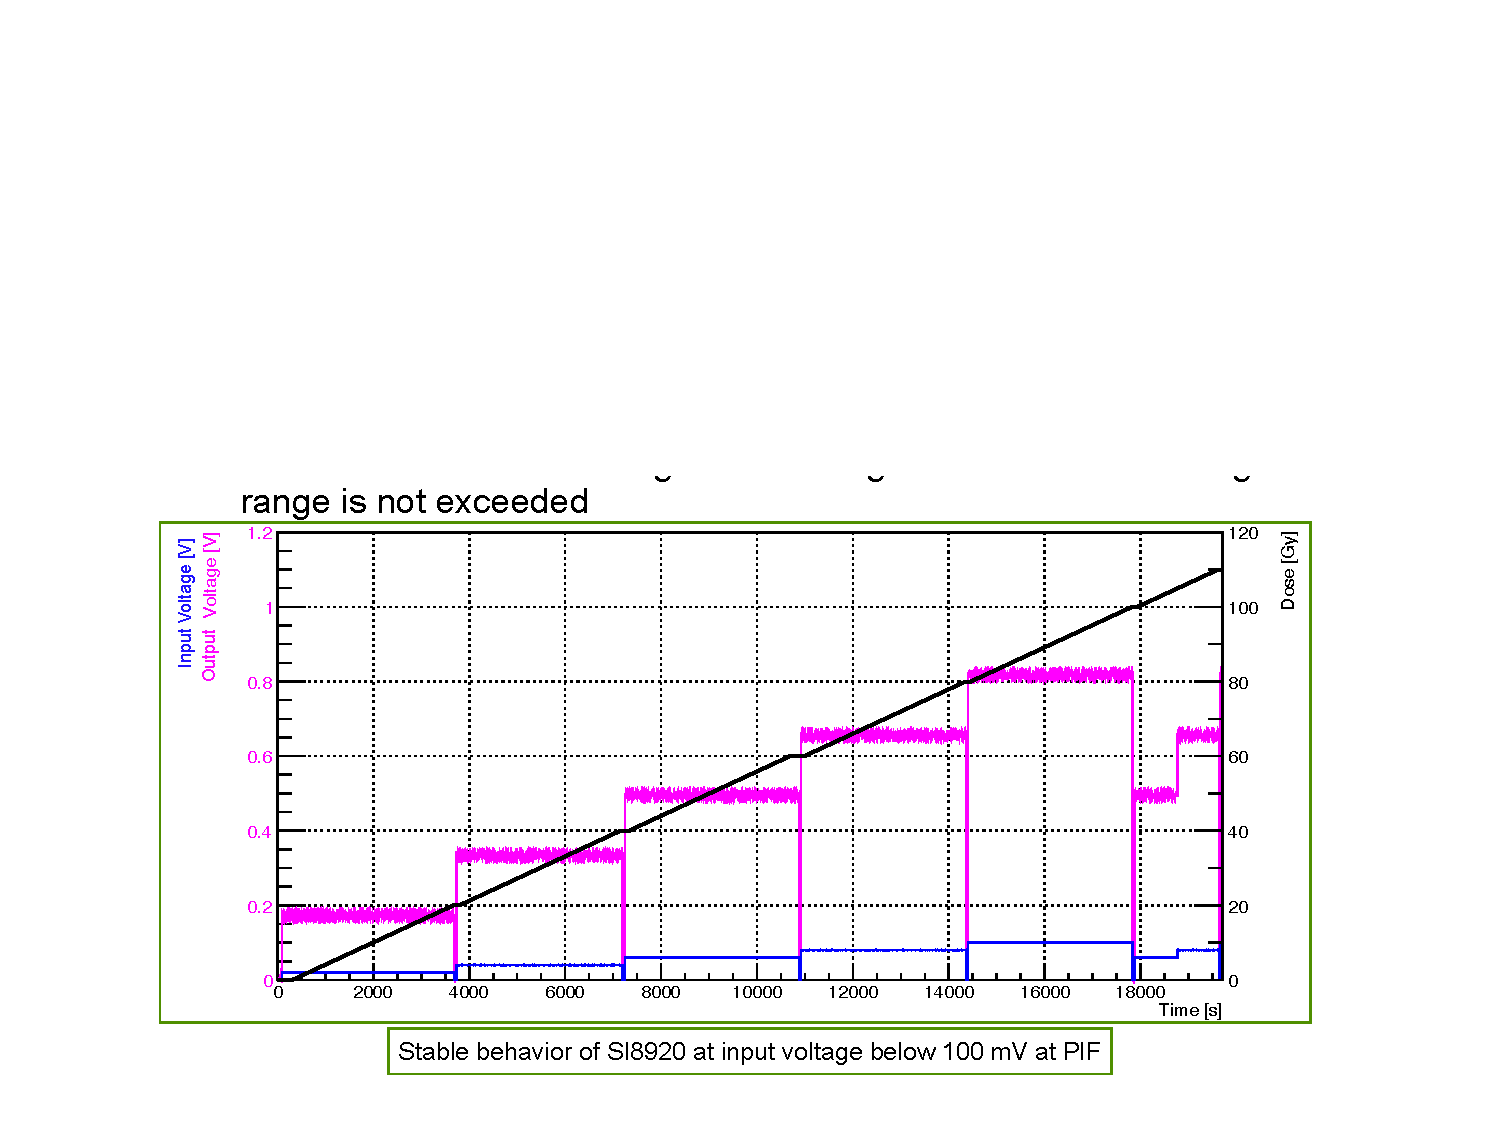
\includegraphics[width=0.8\linewidth]{assets/ATL-TILECAL-SLIDE-2025-552_slide_16_item_2.pdf}
\end{figure}

Seyedali Moayedi

Topical Workshop on Electronics for Particle Physics -- 8 October 2025

16

\section*{Slide 17}

\begin{figure}[H]
\centering

\includegraphics[width=0.8\linewidth]{assets/ATL-TILECAL-SLIDE-2025-552_slide_17_item_1.png}
\end{figure}

Radiation Tests: HCPL7800 Isolation Amp (1)

   This chip was not originally in the design, but was considered after    
initial failures of the original isolation amplifier

   TID and SEE tests performed together at a flux of 2.1 x 10 8  p/cm 2 /s up

   Some SETs were observed on the output voltages, with small amplitude  
(\textasciitilde{}100 mV) and short time (\textasciitilde{}5 us), but as they will be filtered by low-pass  
filters on the brick ,  the chip passed the SEE tests

   There were also no changes in parameters due to TID

   For NIEL tests , samples irradiated up to 8 x 10 12  n/cm 2  at JSI showed  
failure, but  the ones irradiated up to 5 x 10 12  n/cm 2  were working fine

\begin{figure}[H]
\centering
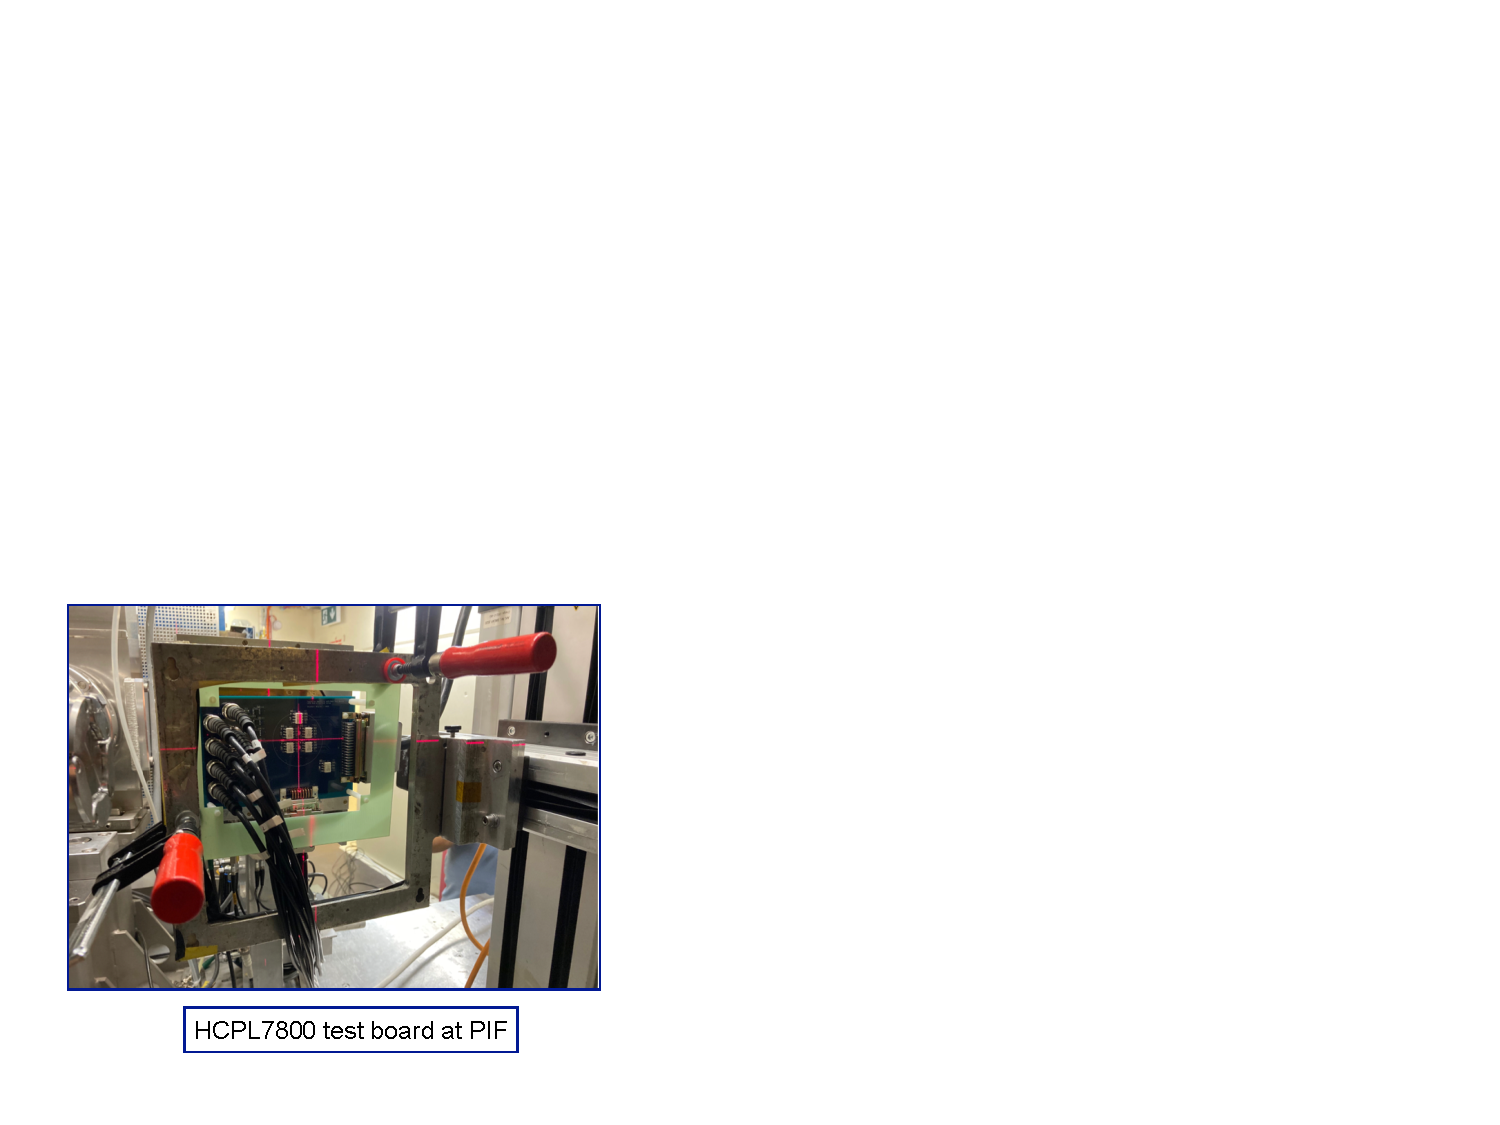
\includegraphics[width=0.8\linewidth]{assets/ATL-TILECAL-SLIDE-2025-552_slide_17_item_2.pdf}
\end{figure}

\begin{figure}[H]
\centering
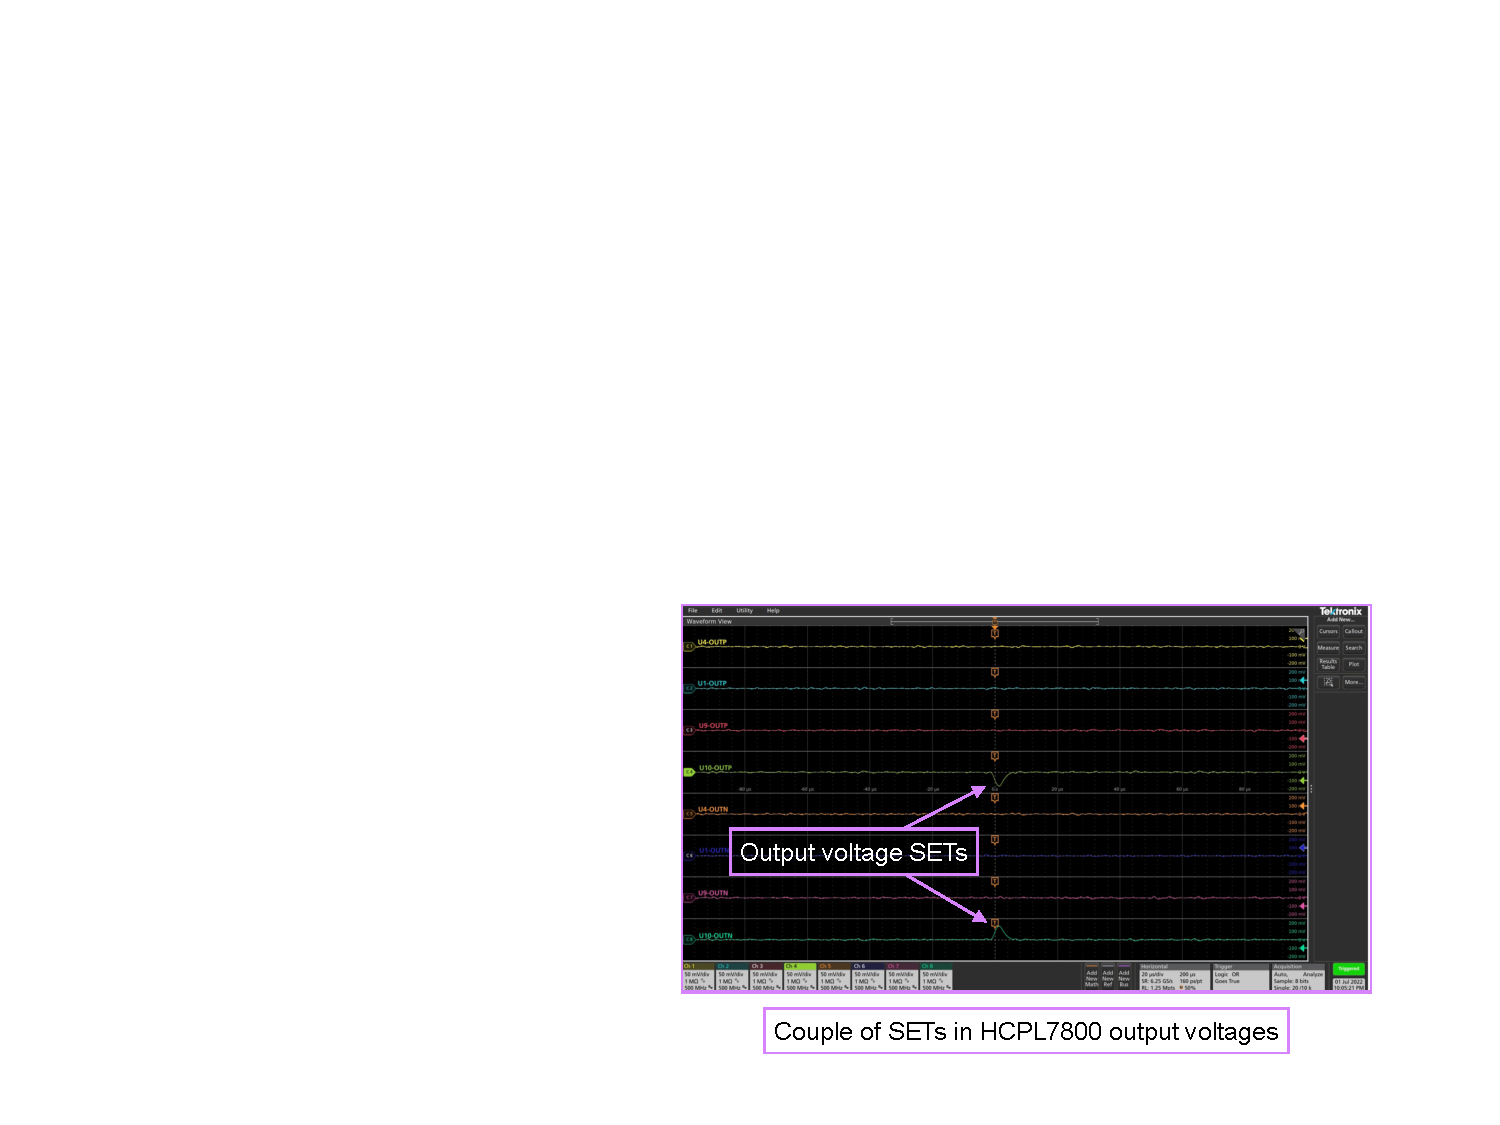
\includegraphics[width=0.8\linewidth]{assets/ATL-TILECAL-SLIDE-2025-552_slide_17_item_3.pdf}
\end{figure}

\begin{figure}[H]
\centering
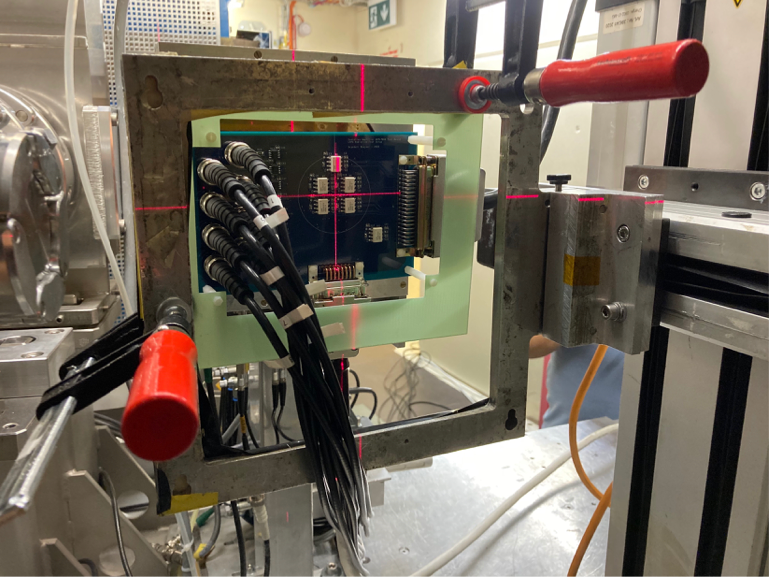
\includegraphics[width=0.8\linewidth]{assets/ATL-TILECAL-SLIDE-2025-552_slide_17_item_4.png}
\end{figure}

\begin{figure}[H]
\centering
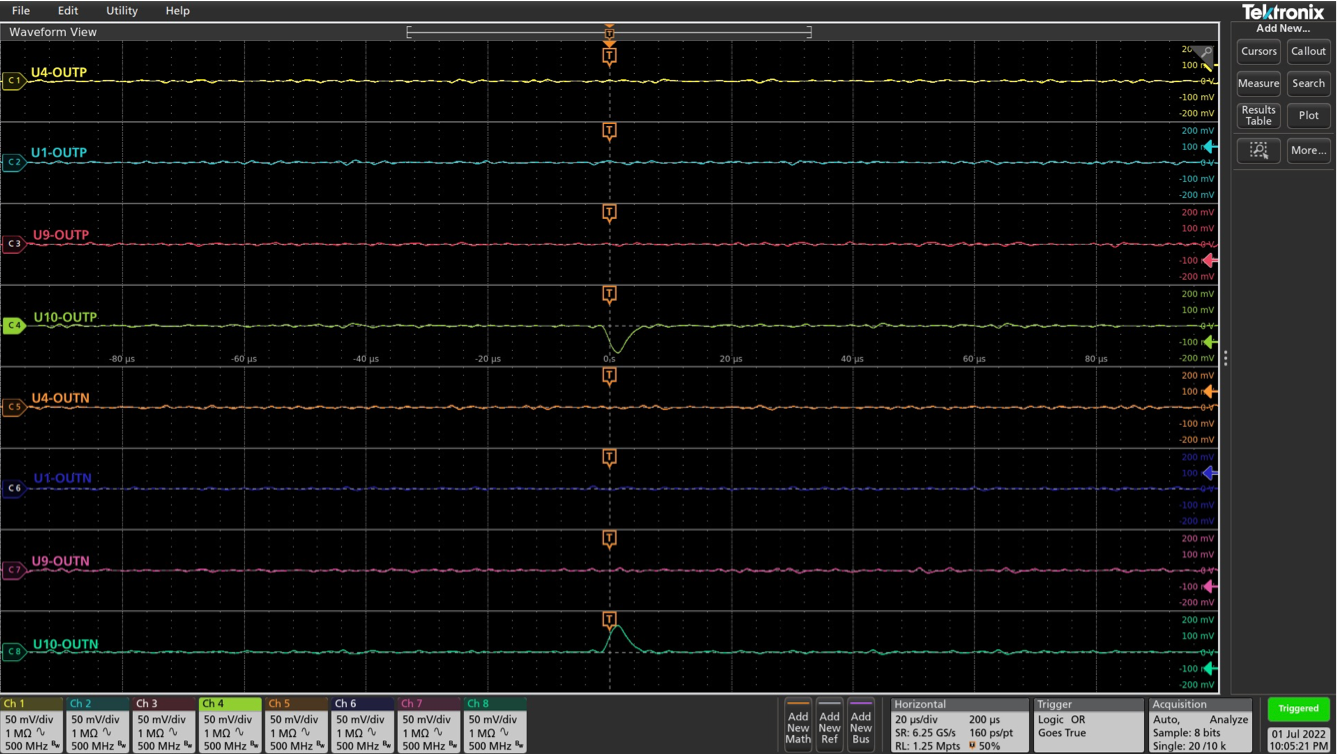
\includegraphics[width=0.8\linewidth]{assets/ATL-TILECAL-SLIDE-2025-552_slide_17_item_5.png}
\end{figure}

Seyedali Moayedi

Topical Workshop on Electronics for Particle Physics -- 8 October 2025

17

\section*{Slide 18}

\begin{figure}[H]
\centering

\includegraphics[width=0.8\linewidth]{assets/ATL-TILECAL-SLIDE-2025-552_slide_18_item_1.png}
\end{figure}

Radiation Tests: HCPL7800 Isolation Amp (2)

   The chip was considered a suitable option for bricks in the modules of  
the end-caps

   The chip was retested as a part of system level tests at CHARM facility,  
before the start of pre-production, and  showed displacement damage  
at only 2.75 x 10 12  n/cm 2

   This chip has bipolar technology, but the results showed that this  
component failed at a lower dose in the mixed field of CHARM  
compared to our tests in TRIGA reactor

   The pre-production started using HCPL7800 (surface-mount package)

   For using in the modules of the barrel, the through-hole package of this  
chip was considered, along with removing the chip from socket and  
replacing it during shut-downs of HL-LHC

   At the end, SI8920 passed the tests and was chosen for the design

\begin{figure}[H]
\centering
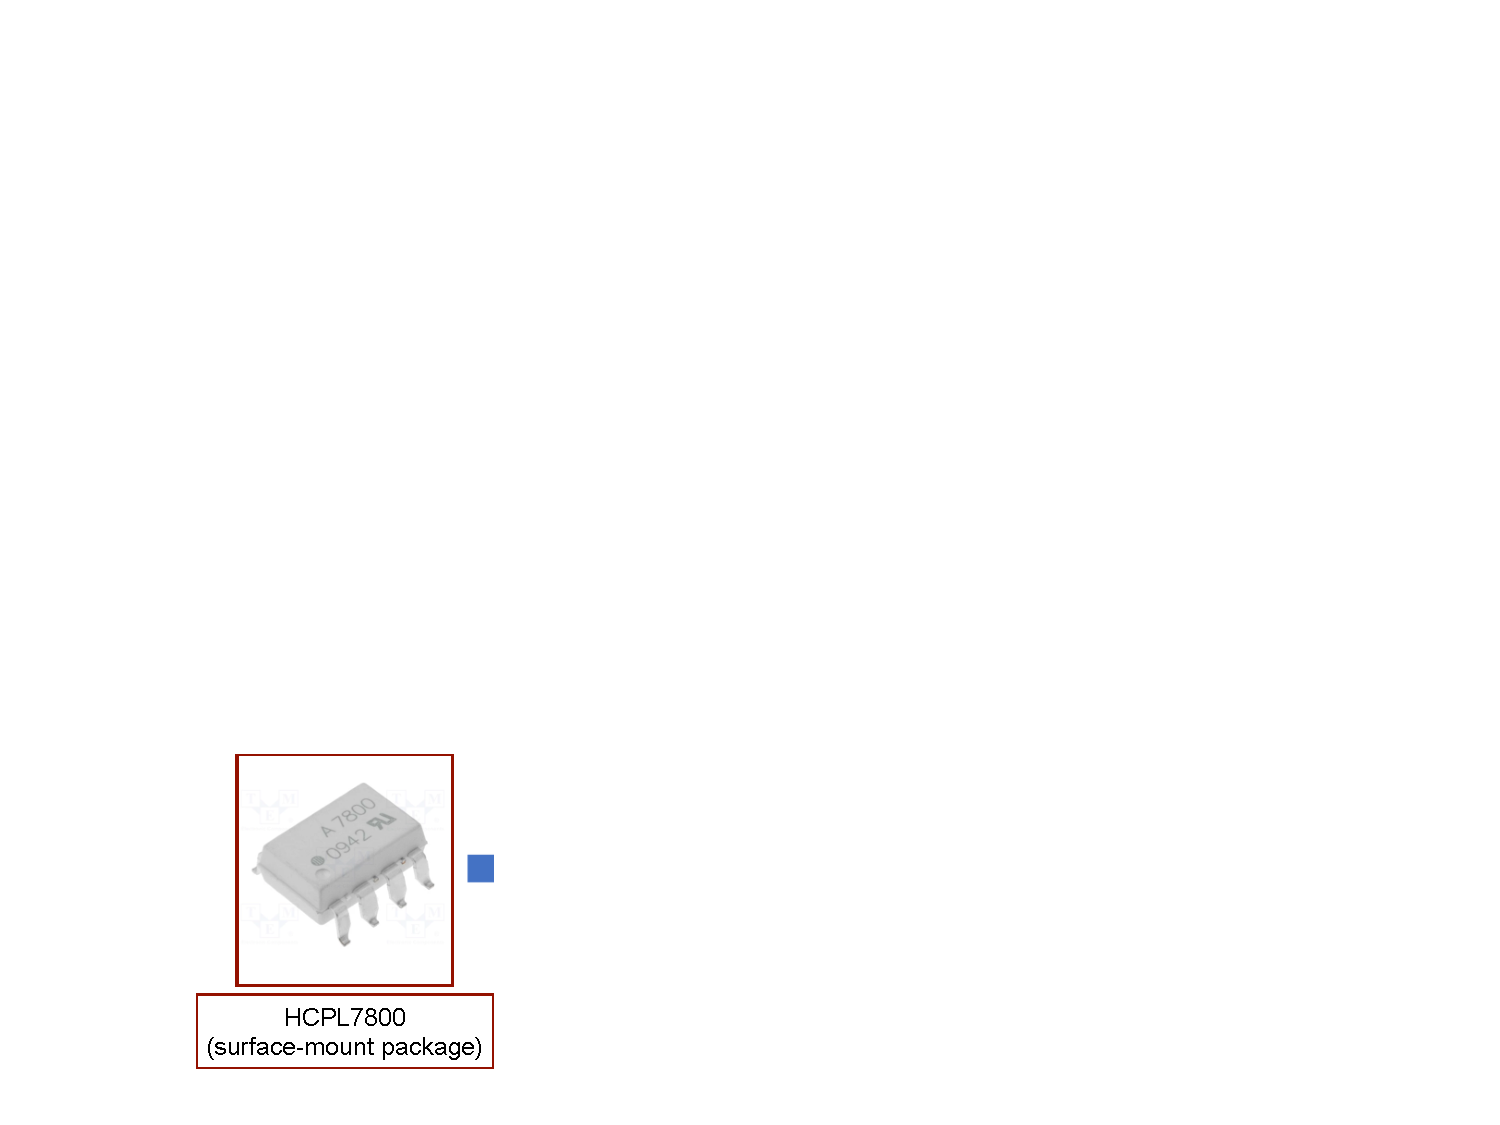
\includegraphics[width=0.8\linewidth]{assets/ATL-TILECAL-SLIDE-2025-552_slide_18_item_2.pdf}
\end{figure}

\begin{figure}[H]
\centering
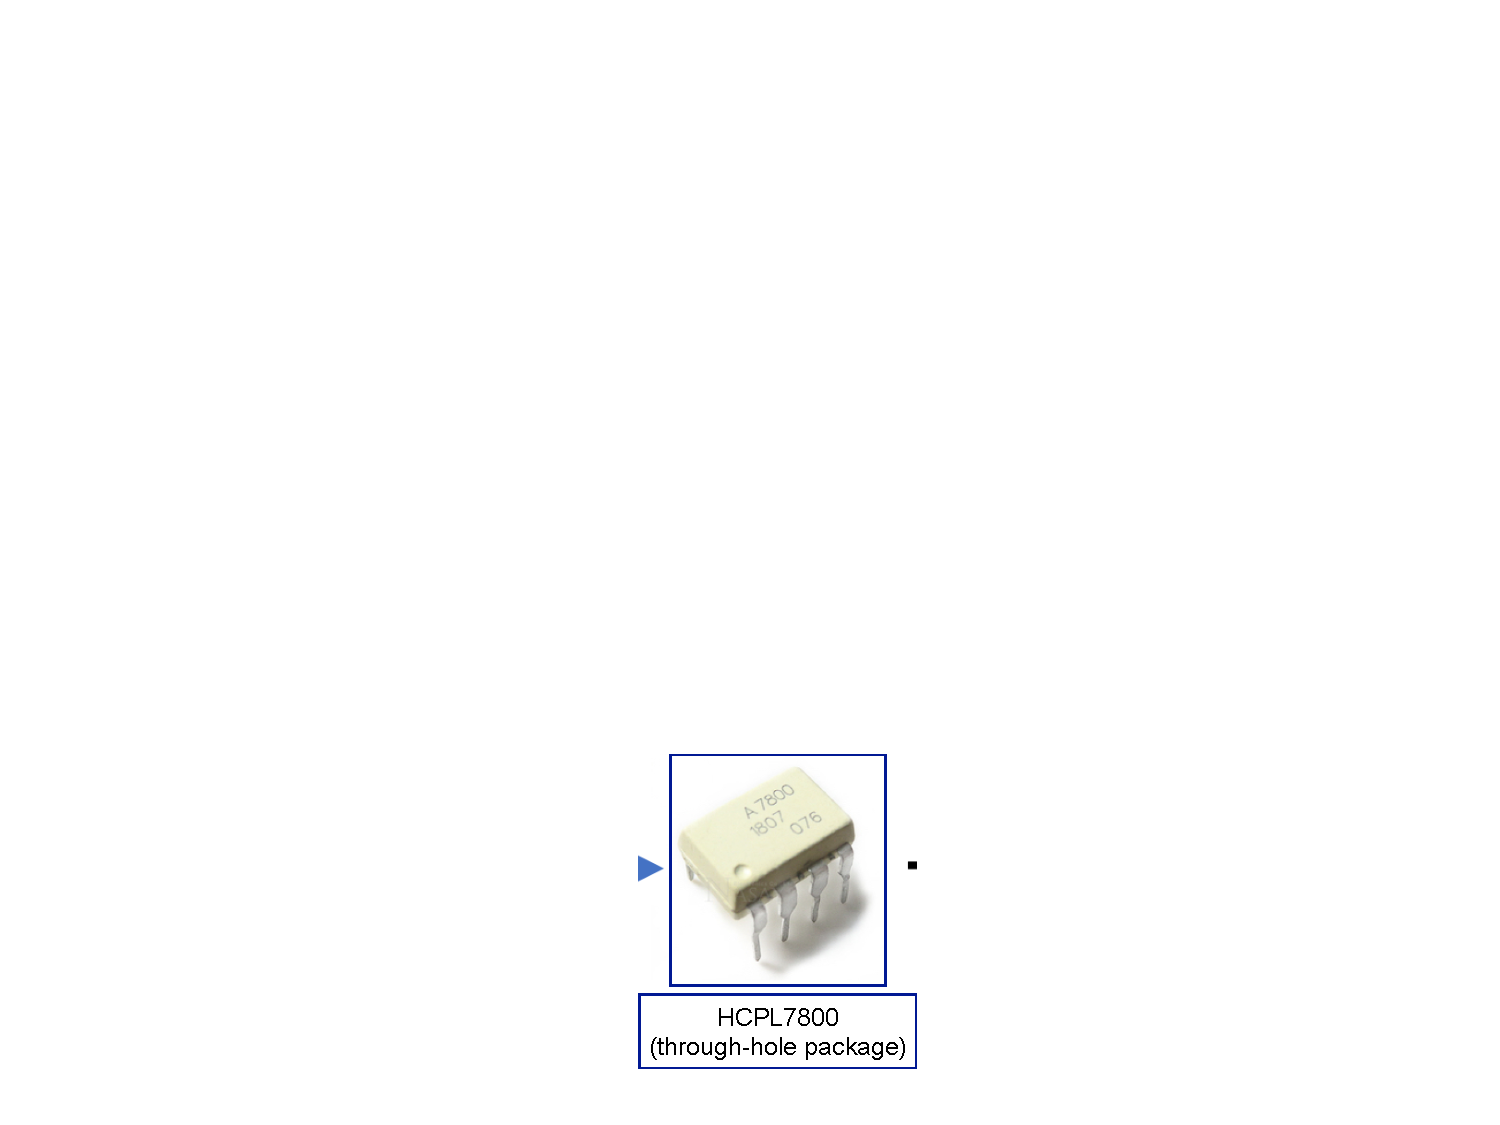
\includegraphics[width=0.8\linewidth]{assets/ATL-TILECAL-SLIDE-2025-552_slide_18_item_3.pdf}
\end{figure}

\begin{figure}[H]
\centering
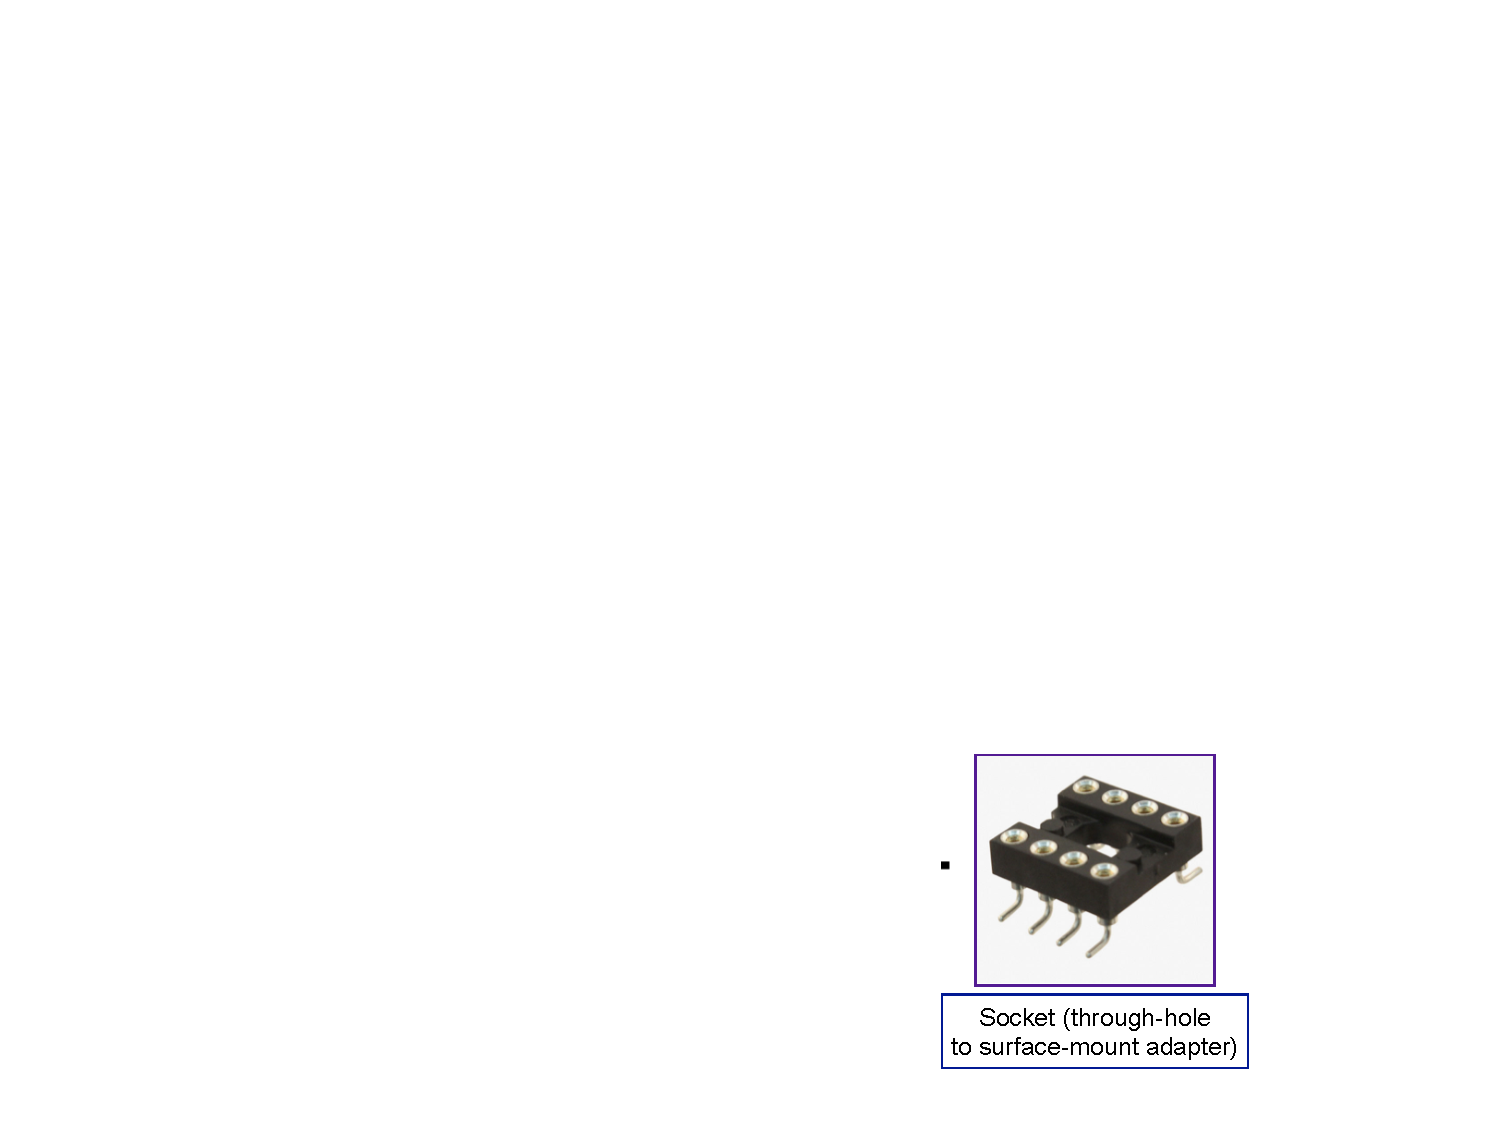
\includegraphics[width=0.8\linewidth]{assets/ATL-TILECAL-SLIDE-2025-552_slide_18_item_4.pdf}
\end{figure}

\begin{figure}[H]
\centering
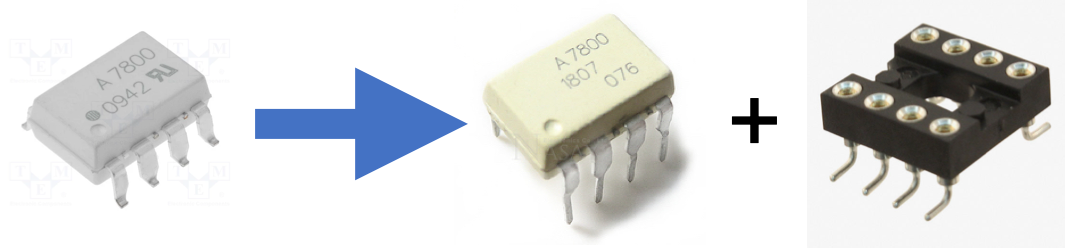
\includegraphics[width=0.8\linewidth]{assets/ATL-TILECAL-SLIDE-2025-552_slide_18_item_5.png}
\end{figure}

Seyedali Moayedi

Topical Workshop on Electronics for Particle Physics -- 8 October 2025

18

\section*{Slide 19}

\begin{figure}[H]
\centering

\includegraphics[width=0.8\linewidth]{assets/ATL-TILECAL-SLIDE-2025-552_slide_19_item_1.png}
\end{figure}

Radiation Tests: System Level Tests (CHARM)

   The entire bricks using HCPL7800 (pre-production version) were    
tested in the mixed field of CHARM facility

   The power MOSFETs failed at a dose of 323 Gy  by having the gate- 
source threshold voltage shifted to zero and creating a short-circuit

   The criteria for this MOSFET is only 80 Gy

   The HCPL7800 amplifier failed at a fluence of 2.75 x 10 12  n/cm 2  due  
to displacement damage

\begin{figure}[H]
\centering
\includegraphics[width=0.8\linewidth]{assets/ATL-TILECAL-SLIDE-2025-552_slide_19_item_2.pdf}
\end{figure}

\begin{figure}[H]
\centering
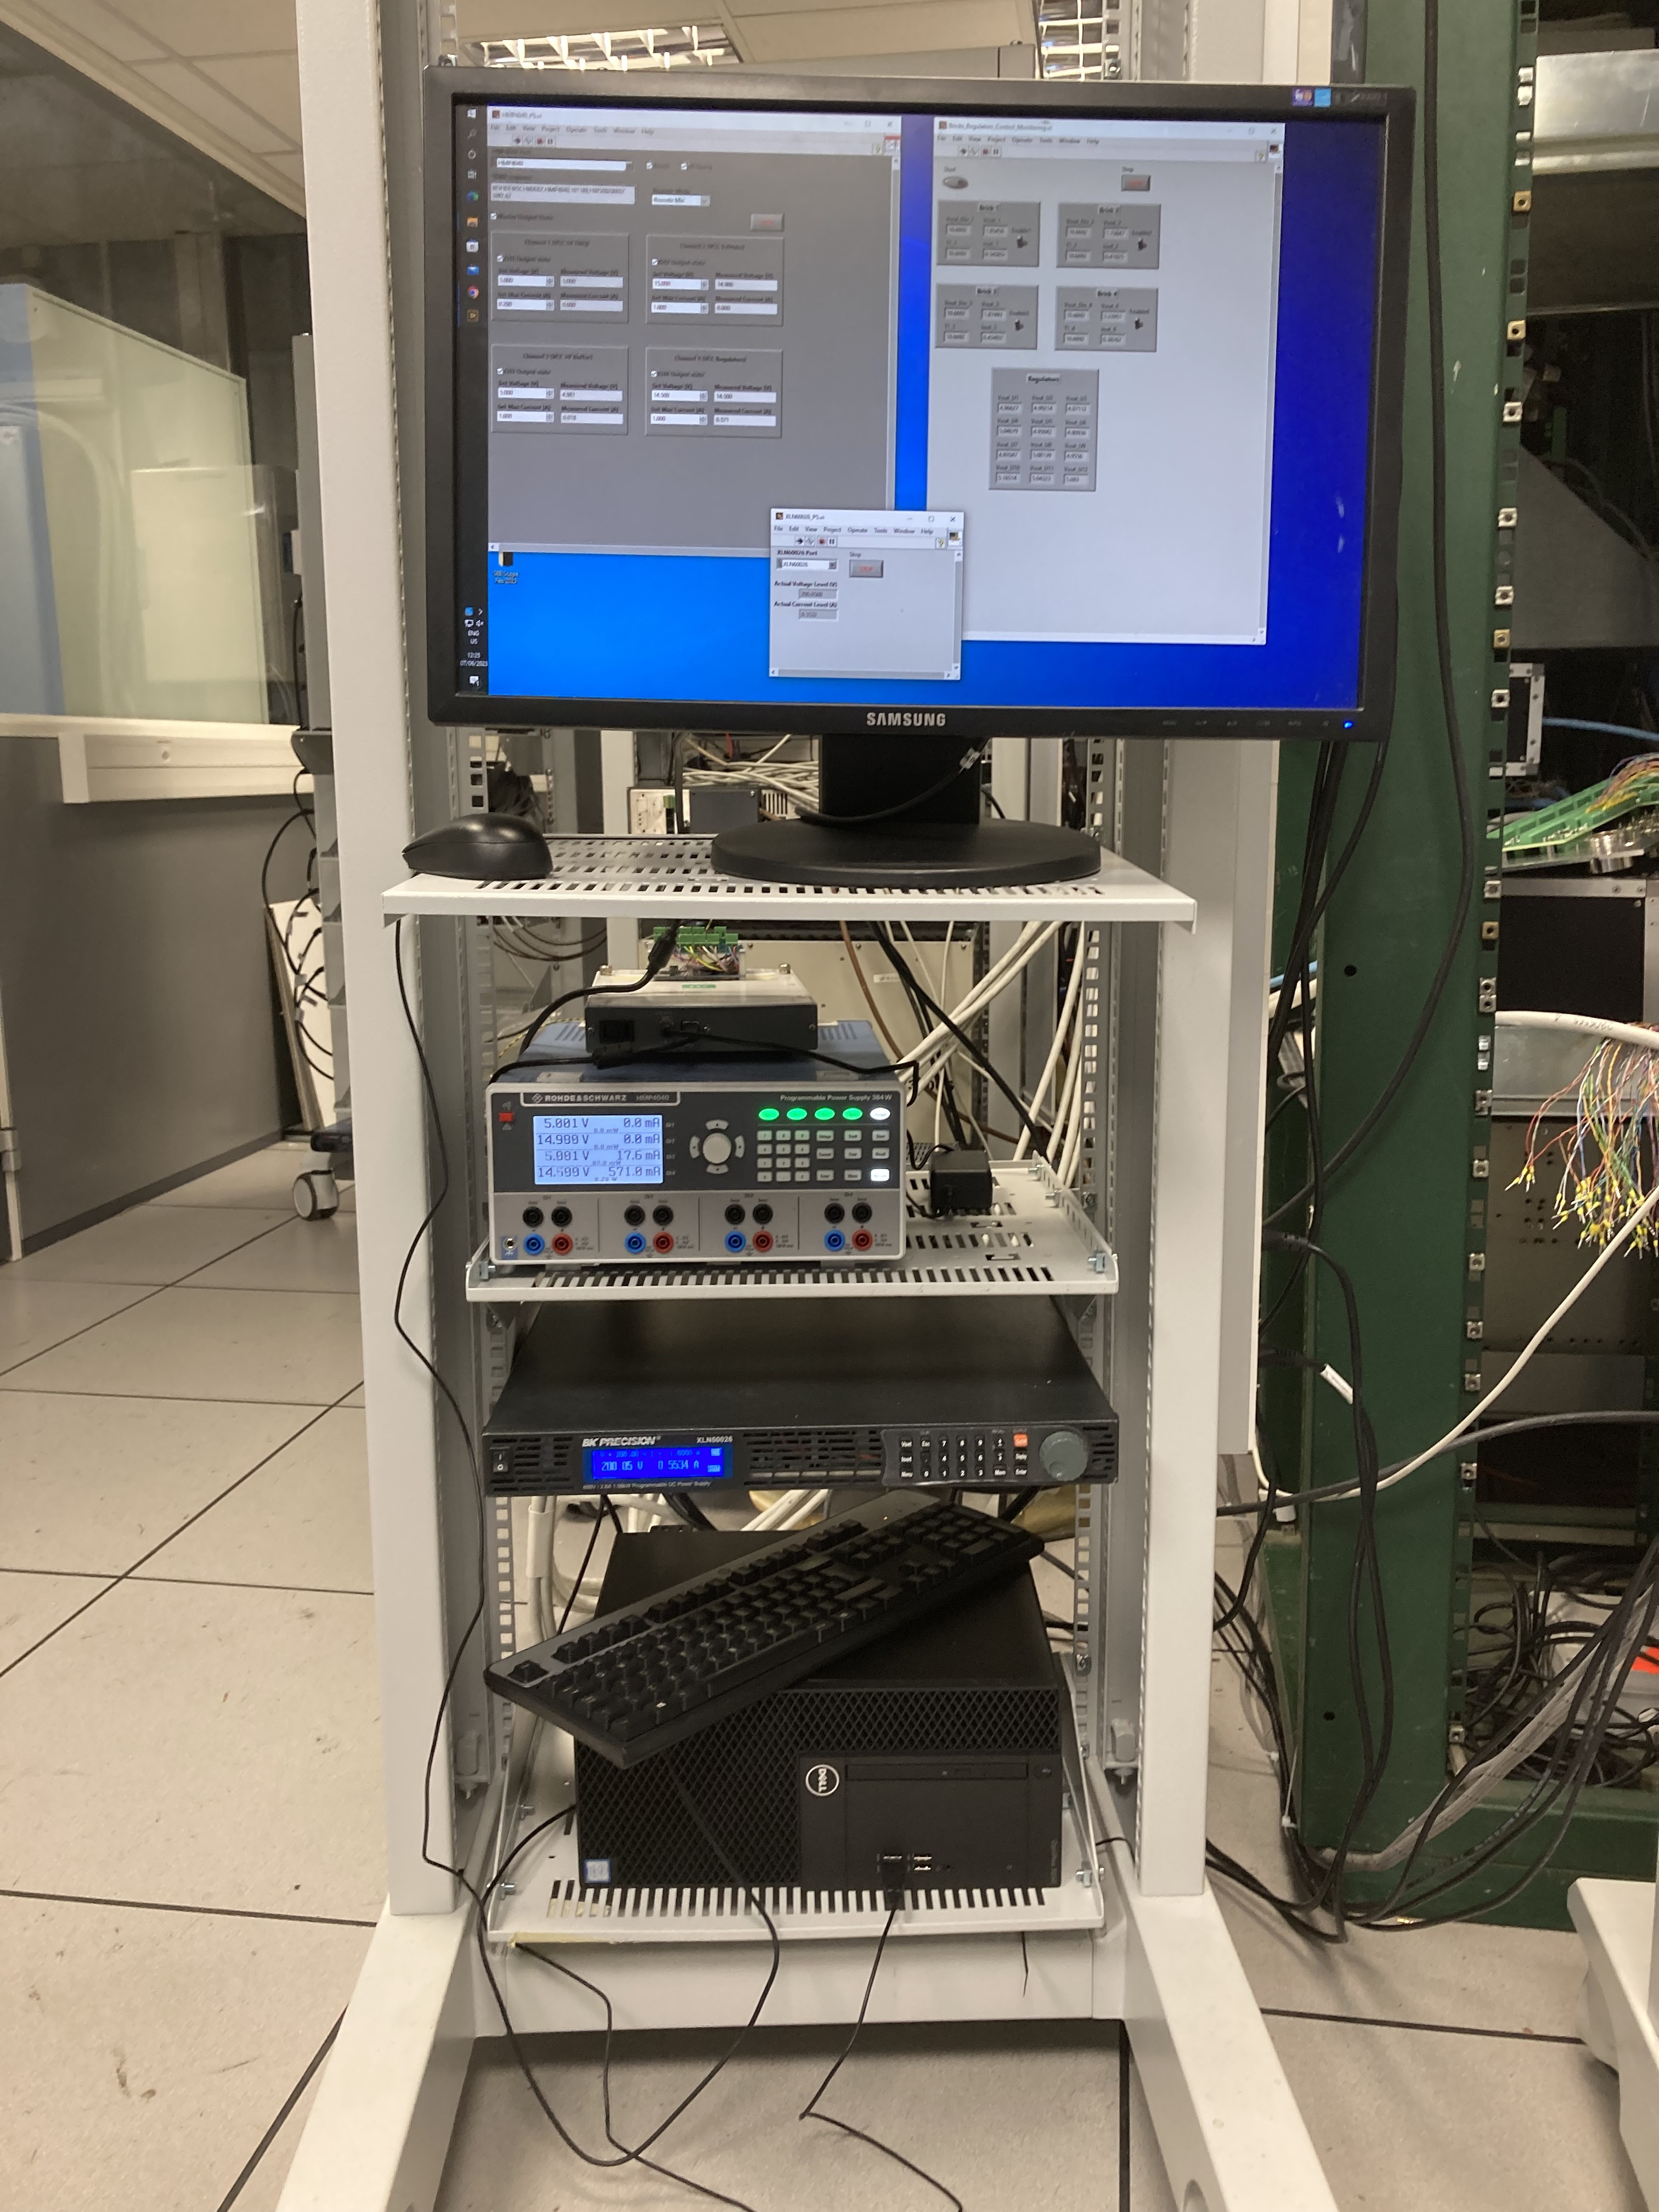
\includegraphics[width=0.8\linewidth]{assets/ATL-TILECAL-SLIDE-2025-552_slide_19_item_3.jpeg}
\end{figure}

\begin{figure}[H]
\centering
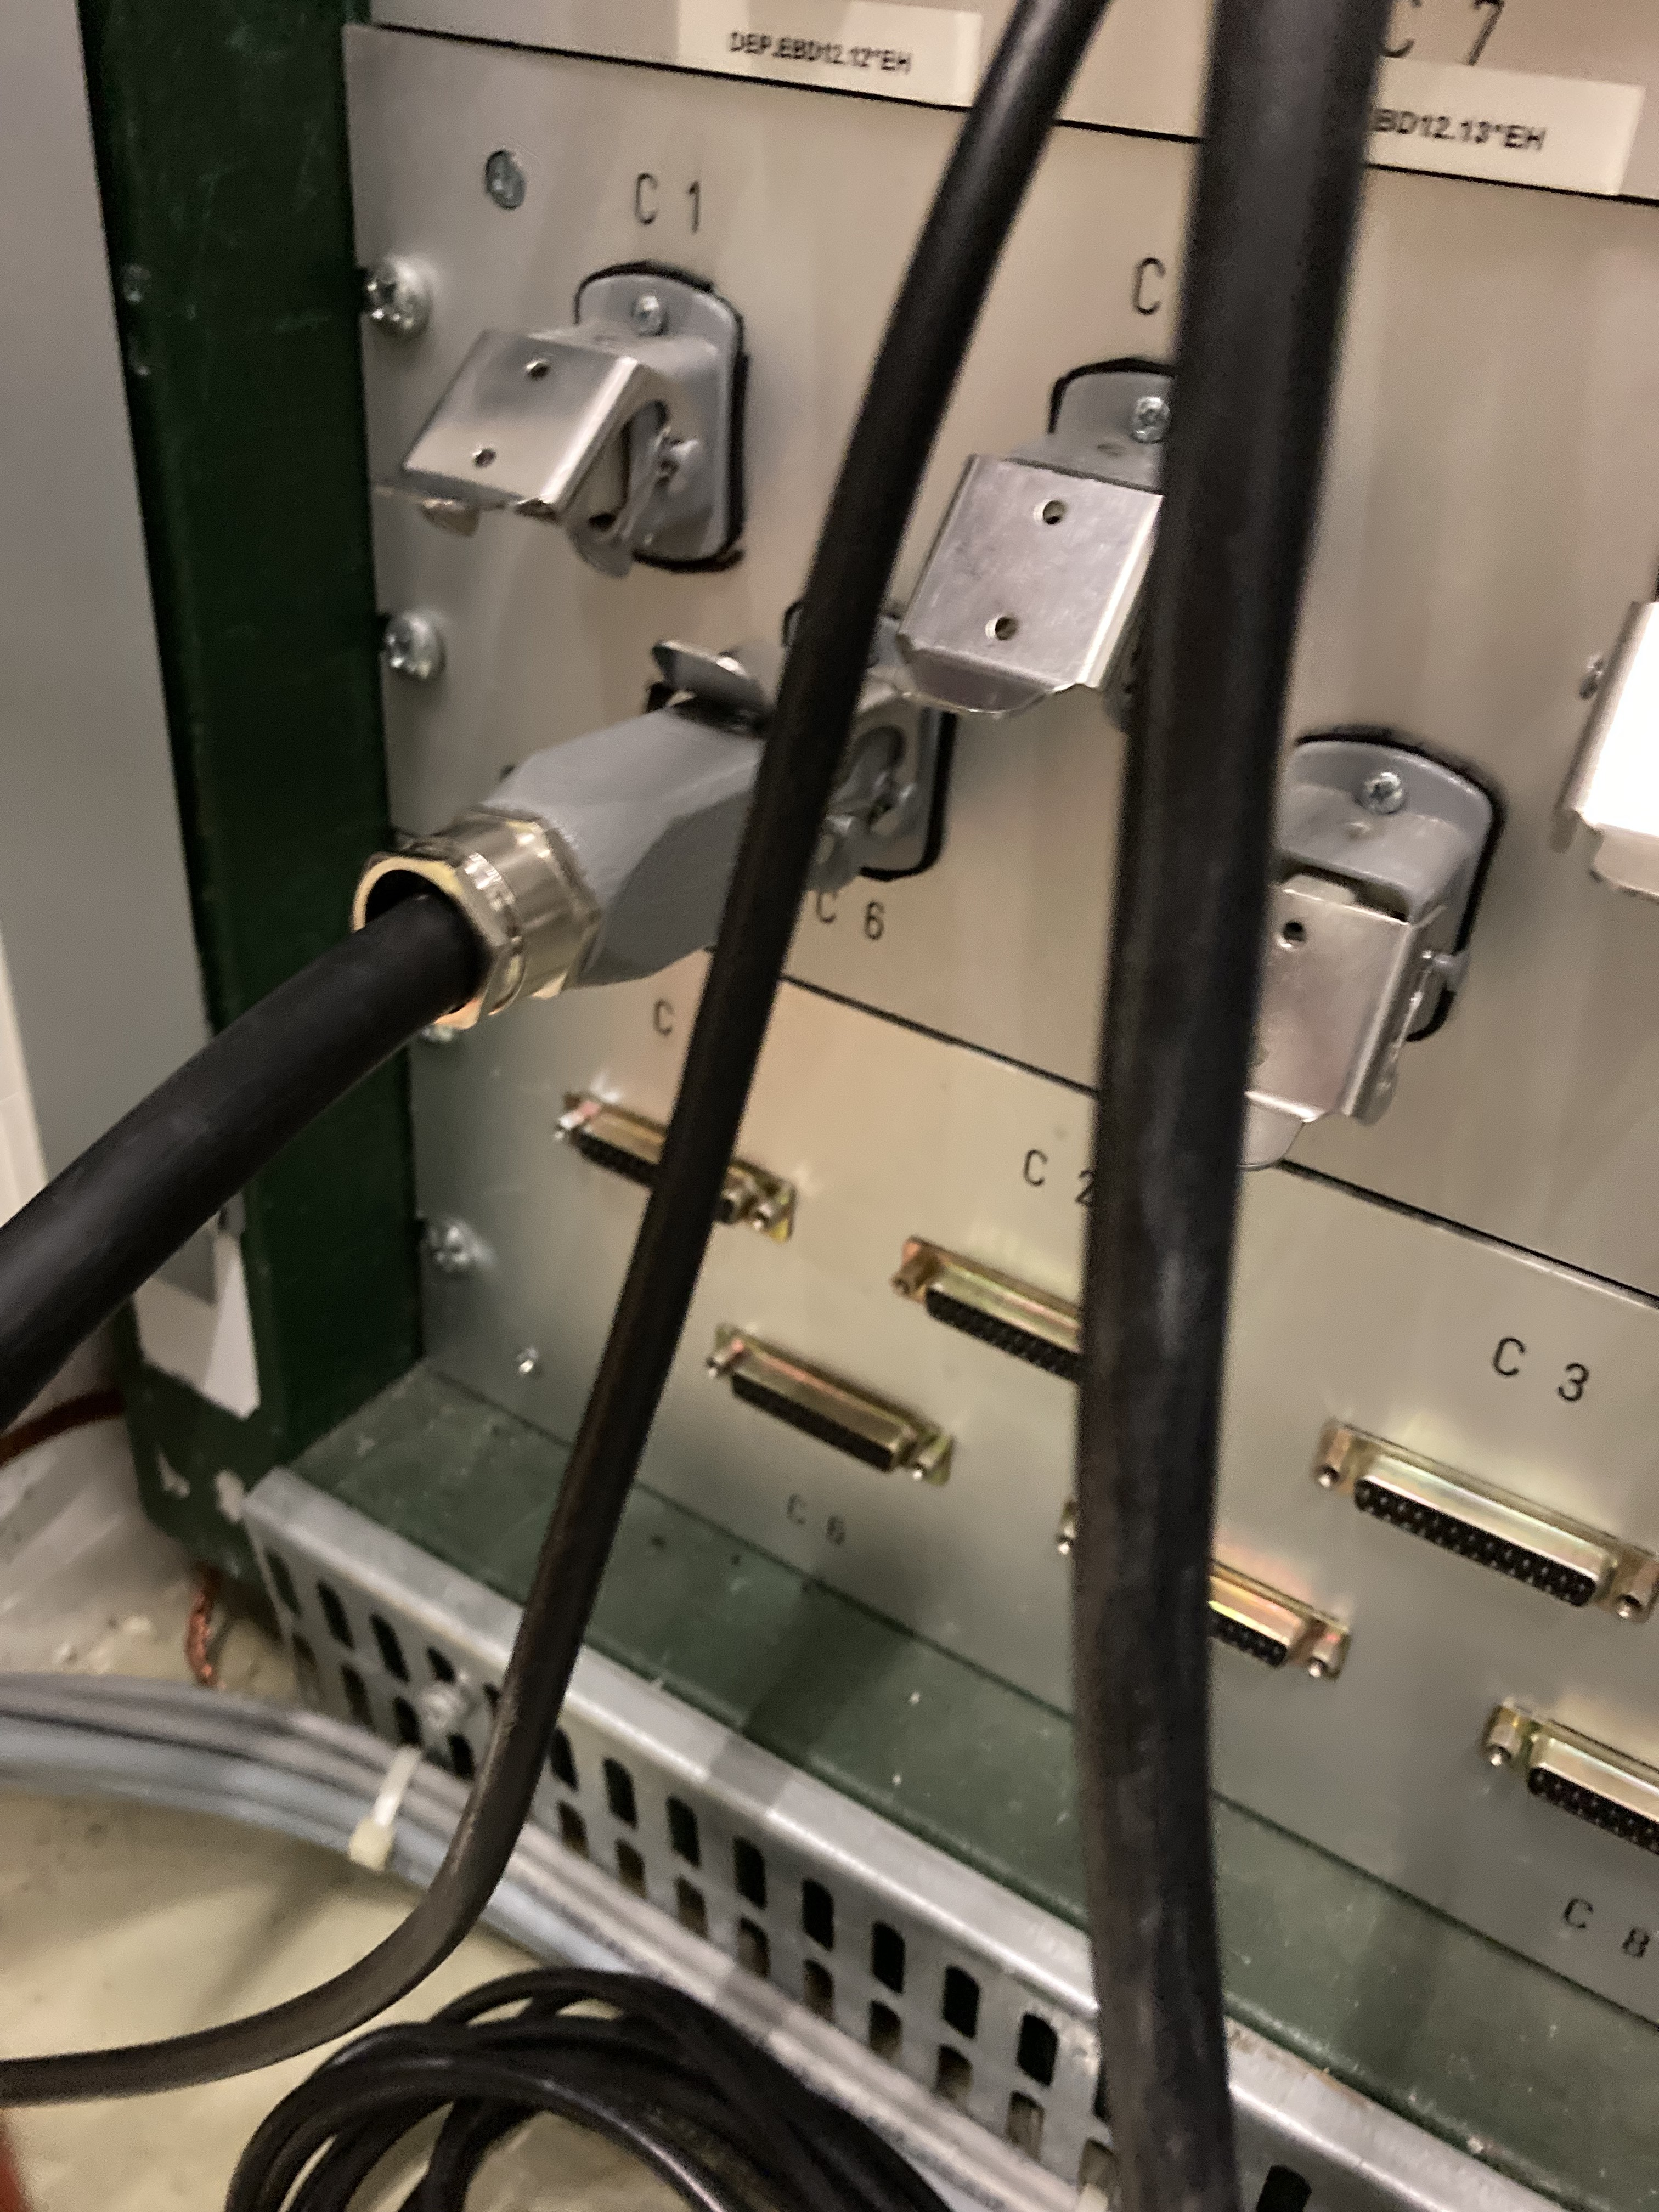
\includegraphics[width=0.8\linewidth]{assets/ATL-TILECAL-SLIDE-2025-552_slide_19_item_4.jpeg}
\end{figure}

\begin{figure}[H]
\centering
\includegraphics[width=0.8\linewidth]{assets/ATL-TILECAL-SLIDE-2025-552_slide_19_item_5.pdf}
\end{figure}

\begin{figure}[H]
\centering
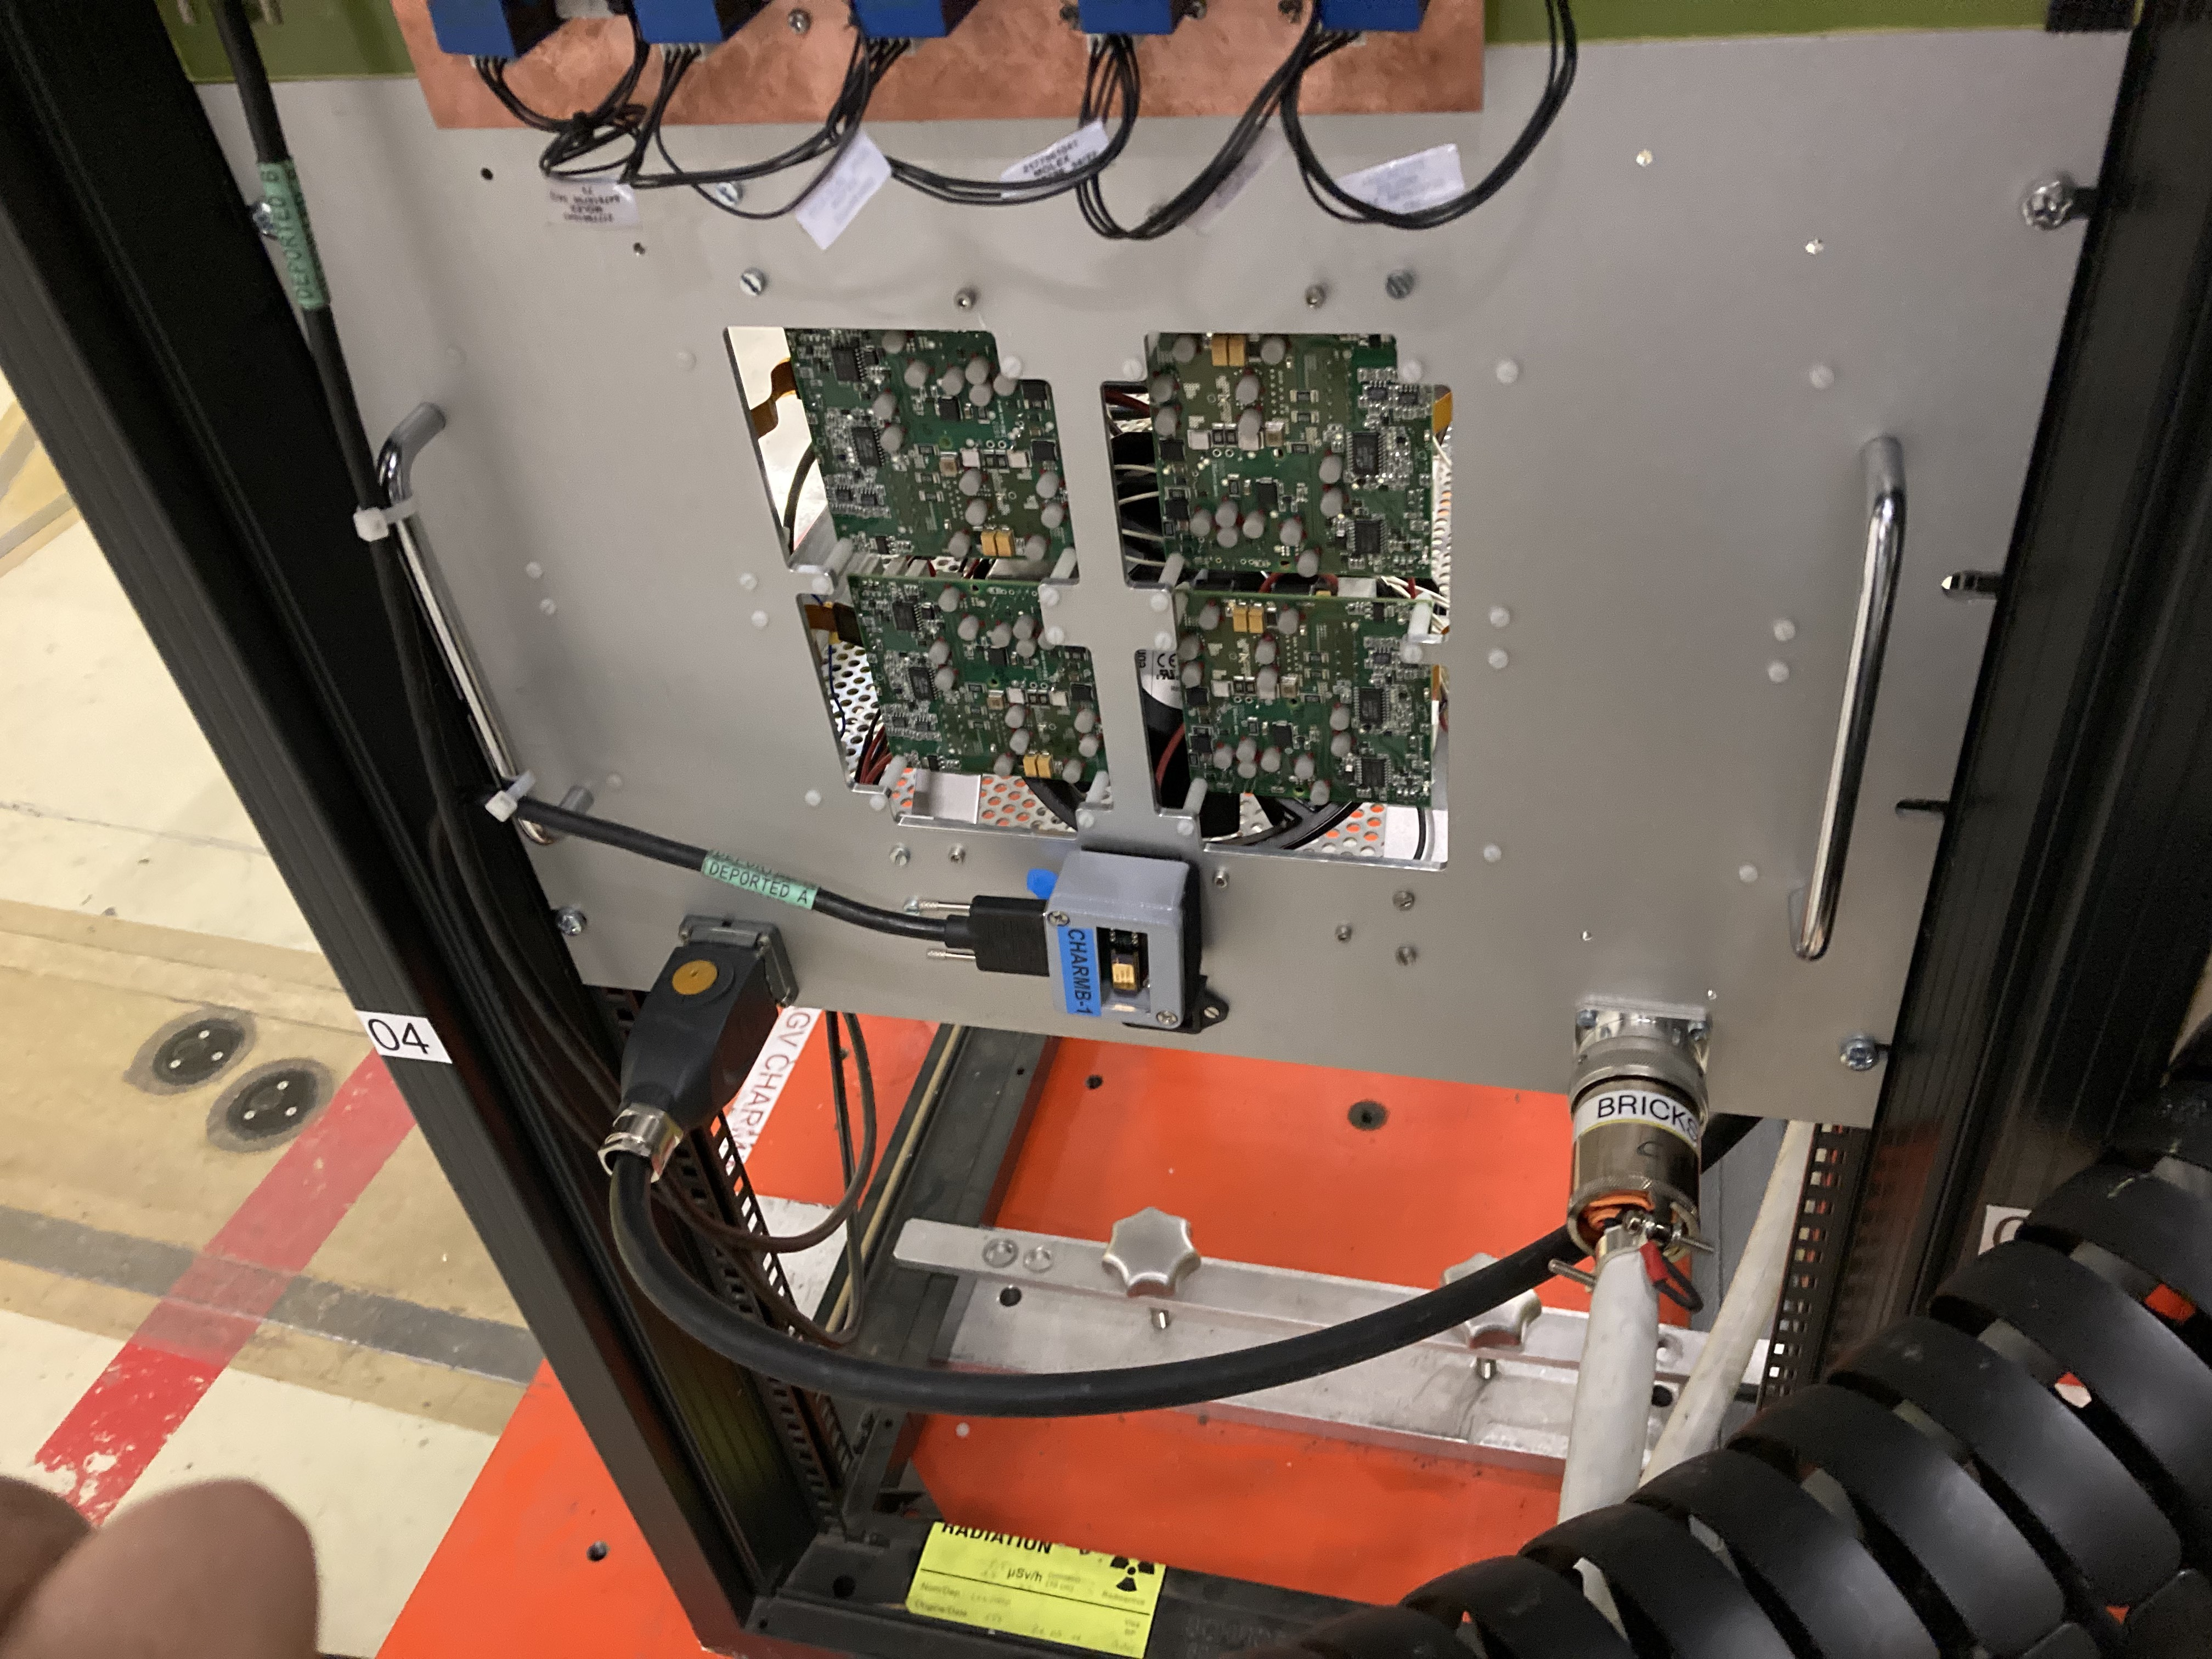
\includegraphics[width=0.8\linewidth]{assets/ATL-TILECAL-SLIDE-2025-552_slide_19_item_6.jpeg}
\end{figure}

\begin{figure}[H]
\centering
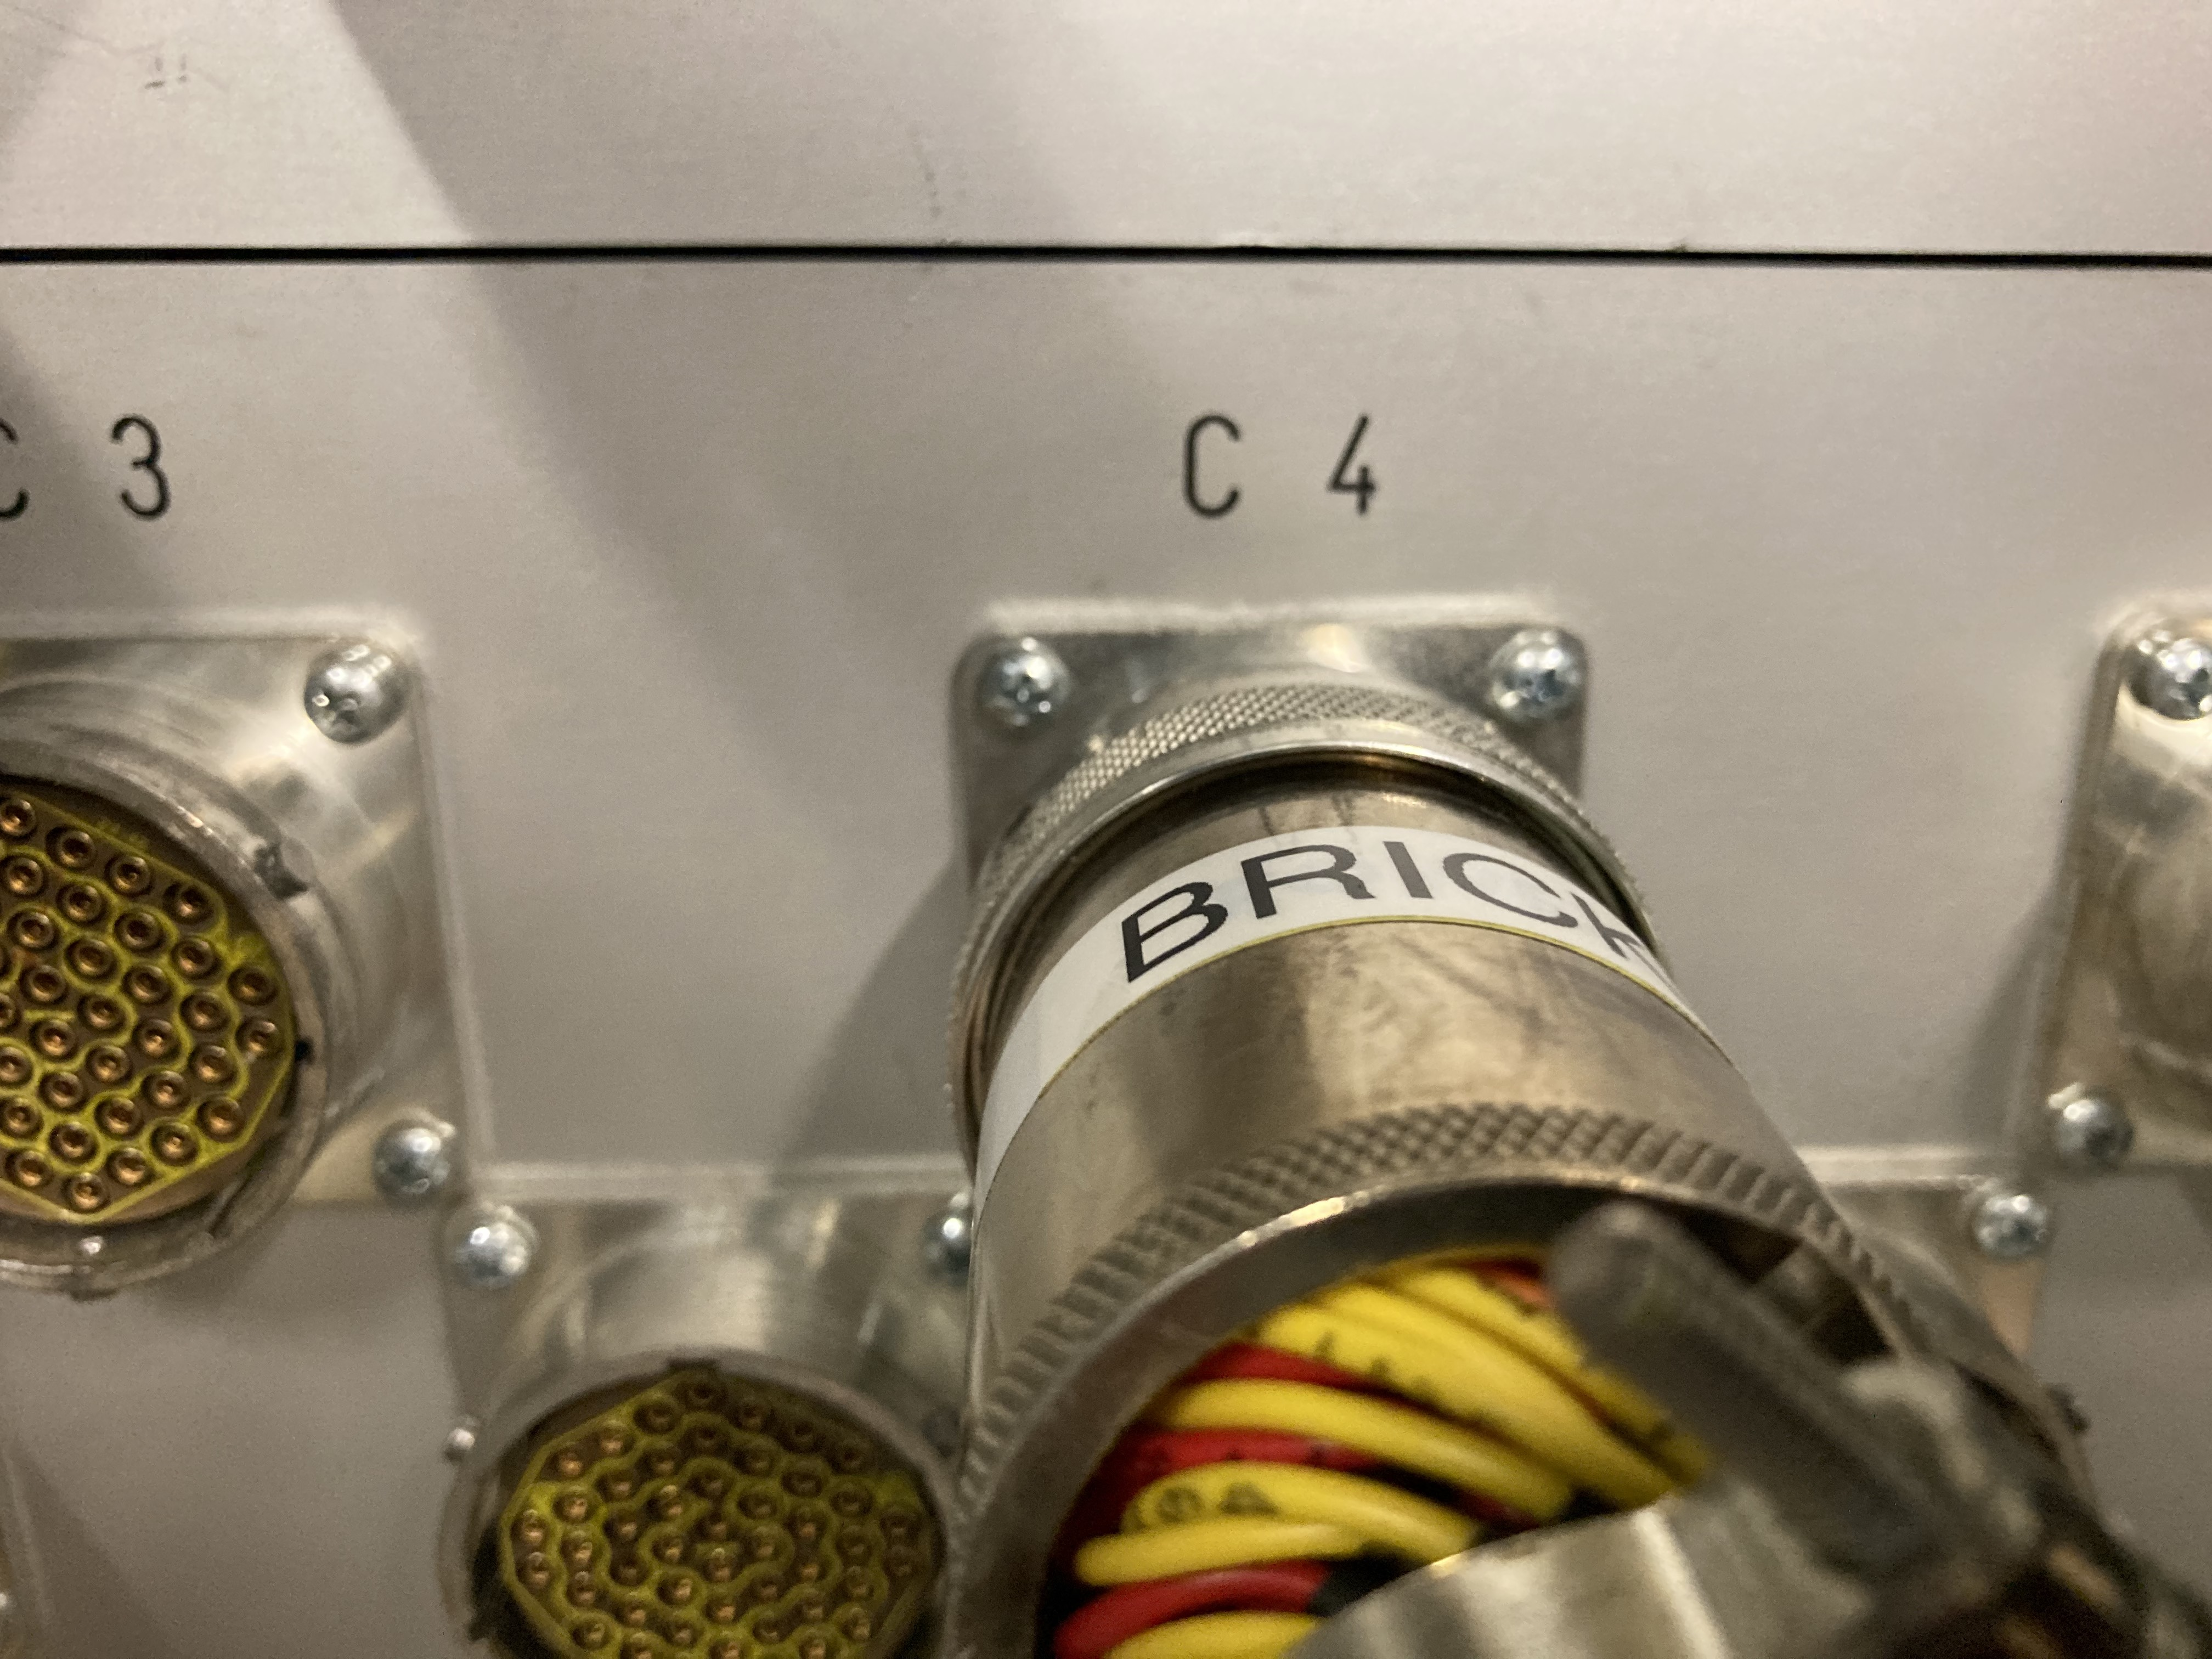
\includegraphics[width=0.8\linewidth]{assets/ATL-TILECAL-SLIDE-2025-552_slide_19_item_7.jpeg}
\end{figure}

Seyedali Moayedi

Topical Workshop on Electronics for Particle Physics -- 8 October 2025

19

\section*{Slide 20}

\begin{figure}[H]
\centering

\includegraphics[width=0.8\linewidth]{assets/ATL-TILECAL-SLIDE-2025-552_slide_20_item_1.png}
\end{figure}

Summary

   An improvement of the new LVPS design is the segmentation of the  
power supply into 8 independent bricks, which enhances the reliability of  
the readout systems, and minimizes the impact of a possible failure during  
data taking

   The design of the brick was improved both by increasing efficiency        
and reducing the signals for controlling the brick turning on/off

   All the components were procured from single (limited) batch(es) to  
perform the tests according to the guidelines from RETF2020 and the  
tests were performed on all of them

   The originally selected SI8920 isolation amplifier showed some  
fluctuations during SEE/TID tests and was initially replaced by HCPL7800  
for pre-production

   Further tests showed stable performance of SI8920 in a specific voltage  
range and the final design of the brick was slightly changed accordingly to  
have stability with SI8920

20 
Seyedali Moayedi

Topical Workshop on Electronics for Particle Physics -- 8 October 2025

\section*{Slide 21}

\begin{figure}[H]
\centering

\includegraphics[width=0.8\linewidth]{assets/ATL-TILECAL-SLIDE-2025-552_slide_21_item_1.png}
\end{figure}

References

[1] Technical Design Report for the Phase-II Upgrade of the ATLAS Tile  
Calorimeter,  https://cds.cern.ch/record/2285583/files/CERN- 
LHCC-2017-019.pdf

21 
Seyedali Moayedi

Topical Workshop on Electronics for Particle Physics -- 8 October 2025

\end{document}
